% Options for packages loaded elsewhere
\PassOptionsToPackage{unicode}{hyperref}
\PassOptionsToPackage{hyphens}{url}
\PassOptionsToPackage{dvipsnames,svgnames,x11names}{xcolor}
%
\documentclass[
  letterpaper,
  DIV=11,
  numbers=noendperiod]{scrreprt}

\usepackage{amsmath,amssymb}
\usepackage{iftex}
\ifPDFTeX
  \usepackage[T1]{fontenc}
  \usepackage[utf8]{inputenc}
  \usepackage{textcomp} % provide euro and other symbols
\else % if luatex or xetex
  \usepackage{unicode-math}
  \defaultfontfeatures{Scale=MatchLowercase}
  \defaultfontfeatures[\rmfamily]{Ligatures=TeX,Scale=1}
\fi
\usepackage{lmodern}
\ifPDFTeX\else  
    % xetex/luatex font selection
\fi
% Use upquote if available, for straight quotes in verbatim environments
\IfFileExists{upquote.sty}{\usepackage{upquote}}{}
\IfFileExists{microtype.sty}{% use microtype if available
  \usepackage[]{microtype}
  \UseMicrotypeSet[protrusion]{basicmath} % disable protrusion for tt fonts
}{}
\makeatletter
\@ifundefined{KOMAClassName}{% if non-KOMA class
  \IfFileExists{parskip.sty}{%
    \usepackage{parskip}
  }{% else
    \setlength{\parindent}{0pt}
    \setlength{\parskip}{6pt plus 2pt minus 1pt}}
}{% if KOMA class
  \KOMAoptions{parskip=half}}
\makeatother
\usepackage{xcolor}
\setlength{\emergencystretch}{3em} % prevent overfull lines
\setcounter{secnumdepth}{5}
% Make \paragraph and \subparagraph free-standing
\ifx\paragraph\undefined\else
  \let\oldparagraph\paragraph
  \renewcommand{\paragraph}[1]{\oldparagraph{#1}\mbox{}}
\fi
\ifx\subparagraph\undefined\else
  \let\oldsubparagraph\subparagraph
  \renewcommand{\subparagraph}[1]{\oldsubparagraph{#1}\mbox{}}
\fi

\usepackage{color}
\usepackage{fancyvrb}
\newcommand{\VerbBar}{|}
\newcommand{\VERB}{\Verb[commandchars=\\\{\}]}
\DefineVerbatimEnvironment{Highlighting}{Verbatim}{commandchars=\\\{\}}
% Add ',fontsize=\small' for more characters per line
\newenvironment{Shaded}{}{}
\newcommand{\AlertTok}[1]{\textcolor[rgb]{0.58,0.85,0.30}{\textbf{\colorbox[rgb]{0.30,0.12,0.14}{#1}}}}
\newcommand{\AnnotationTok}[1]{\textcolor[rgb]{0.60,0.76,0.47}{#1}}
\newcommand{\AttributeTok}[1]{\textcolor[rgb]{0.78,0.47,0.87}{#1}}
\newcommand{\BaseNTok}[1]{\textcolor[rgb]{0.82,0.60,0.40}{#1}}
\newcommand{\BuiltInTok}[1]{\textcolor[rgb]{0.78,0.47,0.87}{#1}}
\newcommand{\CharTok}[1]{\textcolor[rgb]{0.60,0.76,0.47}{#1}}
\newcommand{\CommentTok}[1]{\textcolor[rgb]{0.36,0.39,0.44}{\textit{#1}}}
\newcommand{\CommentVarTok}[1]{\textcolor[rgb]{0.88,0.42,0.46}{\textit{#1}}}
\newcommand{\ConstantTok}[1]{\textcolor[rgb]{0.82,0.60,0.40}{#1}}
\newcommand{\ControlFlowTok}[1]{\textcolor[rgb]{0.78,0.47,0.87}{#1}}
\newcommand{\DataTypeTok}[1]{\textcolor[rgb]{0.78,0.47,0.87}{#1}}
\newcommand{\DecValTok}[1]{\textcolor[rgb]{0.82,0.60,0.40}{#1}}
\newcommand{\DocumentationTok}[1]{\textcolor[rgb]{0.64,0.20,0.25}{#1}}
\newcommand{\ErrorTok}[1]{\textcolor[rgb]{0.96,0.28,0.28}{\underline{#1}}}
\newcommand{\ExtensionTok}[1]{\textcolor[rgb]{0.38,0.69,0.94}{\textbf{#1}}}
\newcommand{\FloatTok}[1]{\textcolor[rgb]{0.82,0.60,0.40}{#1}}
\newcommand{\FunctionTok}[1]{\textcolor[rgb]{0.38,0.69,0.94}{#1}}
\newcommand{\ImportTok}[1]{\textcolor[rgb]{0.60,0.76,0.47}{#1}}
\newcommand{\InformationTok}[1]{\textcolor[rgb]{0.77,0.36,0.00}{#1}}
\newcommand{\KeywordTok}[1]{\textcolor[rgb]{0.78,0.47,0.87}{#1}}
\newcommand{\NormalTok}[1]{\textcolor[rgb]{0.67,0.70,0.75}{#1}}
\newcommand{\OperatorTok}[1]{\textcolor[rgb]{0.78,0.47,0.87}{#1}}
\newcommand{\OtherTok}[1]{\textcolor[rgb]{0.15,0.68,0.38}{#1}}
\newcommand{\PreprocessorTok}[1]{\textcolor[rgb]{0.78,0.47,0.87}{#1}}
\newcommand{\RegionMarkerTok}[1]{\textcolor[rgb]{0.16,0.50,0.73}{\colorbox[rgb]{0.08,0.19,0.26}{#1}}}
\newcommand{\SpecialCharTok}[1]{\textcolor[rgb]{0.34,0.71,0.76}{#1}}
\newcommand{\SpecialStringTok}[1]{\textcolor[rgb]{0.85,0.27,0.33}{#1}}
\newcommand{\StringTok}[1]{\textcolor[rgb]{0.60,0.76,0.47}{#1}}
\newcommand{\VariableTok}[1]{\textcolor[rgb]{0.88,0.42,0.46}{#1}}
\newcommand{\VerbatimStringTok}[1]{\textcolor[rgb]{0.85,0.27,0.33}{#1}}
\newcommand{\WarningTok}[1]{\textcolor[rgb]{0.85,0.27,0.33}{#1}}

\providecommand{\tightlist}{%
  \setlength{\itemsep}{0pt}\setlength{\parskip}{0pt}}\usepackage{longtable,booktabs,array}
\usepackage{calc} % for calculating minipage widths
% Correct order of tables after \paragraph or \subparagraph
\usepackage{etoolbox}
\makeatletter
\patchcmd\longtable{\par}{\if@noskipsec\mbox{}\fi\par}{}{}
\makeatother
% Allow footnotes in longtable head/foot
\IfFileExists{footnotehyper.sty}{\usepackage{footnotehyper}}{\usepackage{footnote}}
\makesavenoteenv{longtable}
\usepackage{graphicx}
\makeatletter
\def\maxwidth{\ifdim\Gin@nat@width>\linewidth\linewidth\else\Gin@nat@width\fi}
\def\maxheight{\ifdim\Gin@nat@height>\textheight\textheight\else\Gin@nat@height\fi}
\makeatother
% Scale images if necessary, so that they will not overflow the page
% margins by default, and it is still possible to overwrite the defaults
% using explicit options in \includegraphics[width, height, ...]{}
\setkeys{Gin}{width=\maxwidth,height=\maxheight,keepaspectratio}
% Set default figure placement to htbp
\makeatletter
\def\fps@figure{htbp}
\makeatother

\usepackage{booktabs}
\usepackage{longtable}
\usepackage{array}
\usepackage{multirow}
\usepackage{wrapfig}
\usepackage{float}
\usepackage{colortbl}
\usepackage{pdflscape}
\usepackage{tabu}
\usepackage{threeparttable}
\usepackage{threeparttablex}
\usepackage[normalem]{ulem}
\usepackage{makecell}
\usepackage{xcolor}
\usepackage{svg}
\KOMAoption{captions}{tableheading}
\makeatletter
\makeatother
\makeatletter
\@ifpackageloaded{bookmark}{}{\usepackage{bookmark}}
\makeatother
\makeatletter
\@ifpackageloaded{caption}{}{\usepackage{caption}}
\AtBeginDocument{%
\ifdefined\contentsname
  \renewcommand*\contentsname{Table of contents}
\else
  \newcommand\contentsname{Table of contents}
\fi
\ifdefined\listfigurename
  \renewcommand*\listfigurename{List of Figures}
\else
  \newcommand\listfigurename{List of Figures}
\fi
\ifdefined\listtablename
  \renewcommand*\listtablename{List of Tables}
\else
  \newcommand\listtablename{List of Tables}
\fi
\ifdefined\figurename
  \renewcommand*\figurename{Figure}
\else
  \newcommand\figurename{Figure}
\fi
\ifdefined\tablename
  \renewcommand*\tablename{Table}
\else
  \newcommand\tablename{Table}
\fi
}
\@ifpackageloaded{float}{}{\usepackage{float}}
\floatstyle{ruled}
\@ifundefined{c@chapter}{\newfloat{codelisting}{h}{lop}}{\newfloat{codelisting}{h}{lop}[chapter]}
\floatname{codelisting}{Listing}
\newcommand*\listoflistings{\listof{codelisting}{List of Listings}}
\makeatother
\makeatletter
\@ifpackageloaded{caption}{}{\usepackage{caption}}
\@ifpackageloaded{subcaption}{}{\usepackage{subcaption}}
\makeatother
\makeatletter
\makeatother
\ifLuaTeX
  \usepackage{selnolig}  % disable illegal ligatures
\fi
\IfFileExists{bookmark.sty}{\usepackage{bookmark}}{\usepackage{hyperref}}
\IfFileExists{xurl.sty}{\usepackage{xurl}}{} % add URL line breaks if available
\urlstyle{same} % disable monospaced font for URLs
\hypersetup{
  pdftitle={A Guide to Interpreting the Results of MetaDAG Analysis},
  colorlinks=true,
  linkcolor={blue},
  filecolor={Maroon},
  citecolor={Blue},
  urlcolor={Blue},
  pdfcreator={LaTeX via pandoc}}

\title{A Guide to Interpreting the Results of MetaDAG Analysis}
\author{}
\date{}

\begin{document}
\maketitle
\renewcommand*\contentsname{Table of contents}
{
\hypersetup{linkcolor=blue}
\setcounter{tocdepth}{2}
\tableofcontents
}
\bookmarksetup{startatroot}

\hypertarget{load-data}{%
\chapter{Load data}\label{load-data}}

As an illustrative example for interpreting
\href{https://bioinfo.uib.es/metadag/}{metaDAG} results, we consider
here the Eukaryotes test presented in Section 2.5. Namely, we consider
all Eukaryotes from the KEGG database.

First of all, results must be downloaded from:

Hash:
\href{https://bioinfo.uib.es/metadag/handleExperiment/result_0a845f74-826e-3b46-aed9-e7ecf74db262}{0a845f74-826e-3b46-aed9-e7ecf74db262}

URL:
(https://bioinfo.uib.es/metadag/handleExperiment/result\_0a845f74-826e-3b46-aed9-e7ecf74db262)

and saved in the folder:

``data/result\_0a845f74-826e-3b46-aed9-e7ecf74db262''.

\begin{Shaded}
\begin{Highlighting}[]
\FunctionTok{library}\NormalTok{(tidyverse)}
\FunctionTok{library}\NormalTok{(igraph)}
\FunctionTok{library}\NormalTok{(ComplexHeatmap)}
\FunctionTok{library}\NormalTok{(viridis)}
\FunctionTok{library}\NormalTok{(circlize)}
\FunctionTok{library}\NormalTok{(plotly)}
\FunctionTok{library}\NormalTok{(randomcoloR)}
\FunctionTok{library}\NormalTok{(factoextra)}
\FunctionTok{library}\NormalTok{(RColorBrewer)}
\FunctionTok{library}\NormalTok{(kableExtra)}
\FunctionTok{library}\NormalTok{(igraph)}
\FunctionTok{library}\NormalTok{(GGally)}
\end{Highlighting}
\end{Shaded}

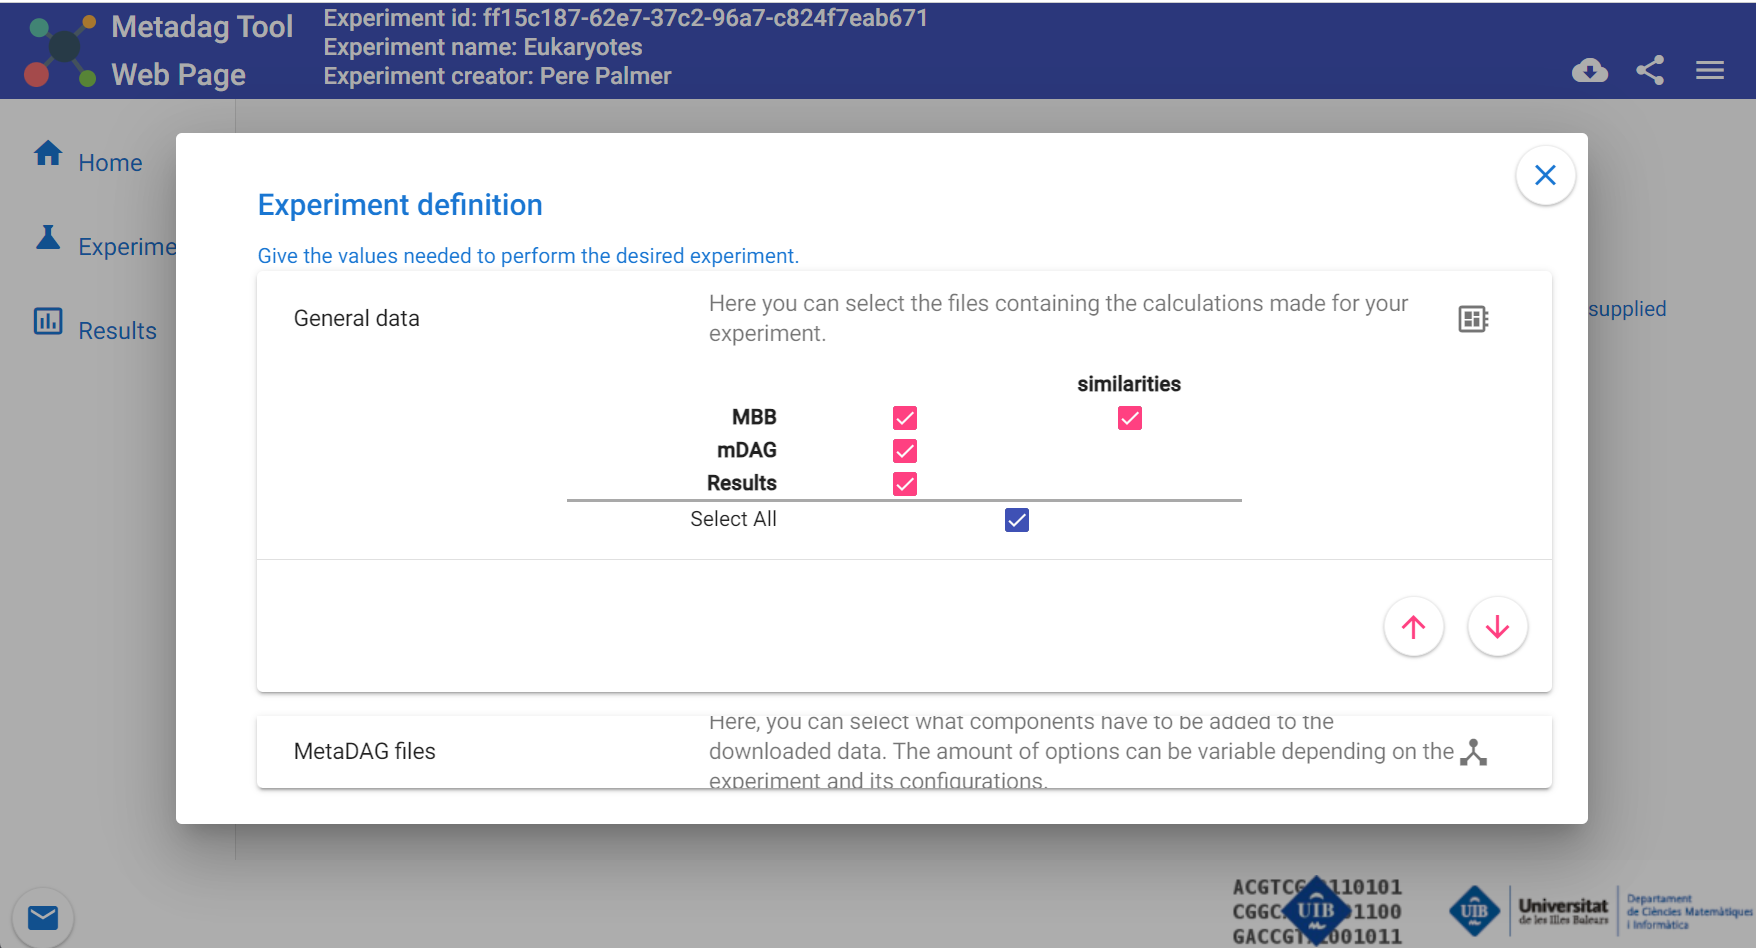
\includegraphics[width=1\textwidth,height=\textheight]{figures/screen_2.png}

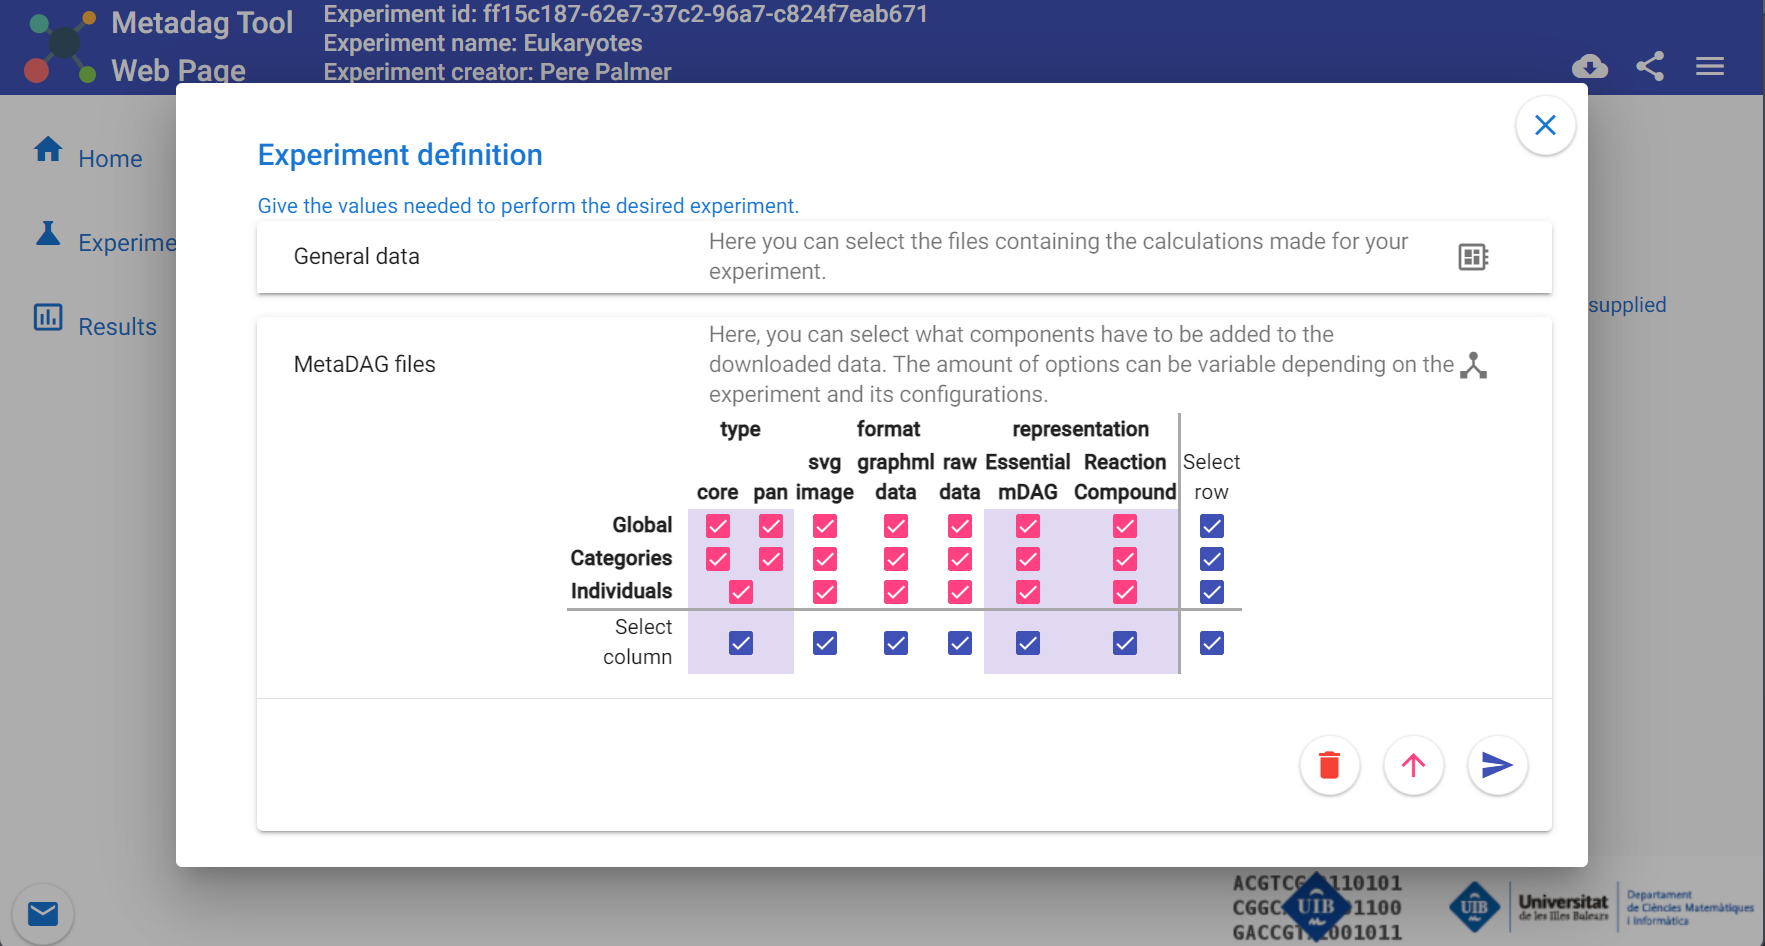
\includegraphics[width=1\textwidth,height=\textheight]{figures/screen_3.png}

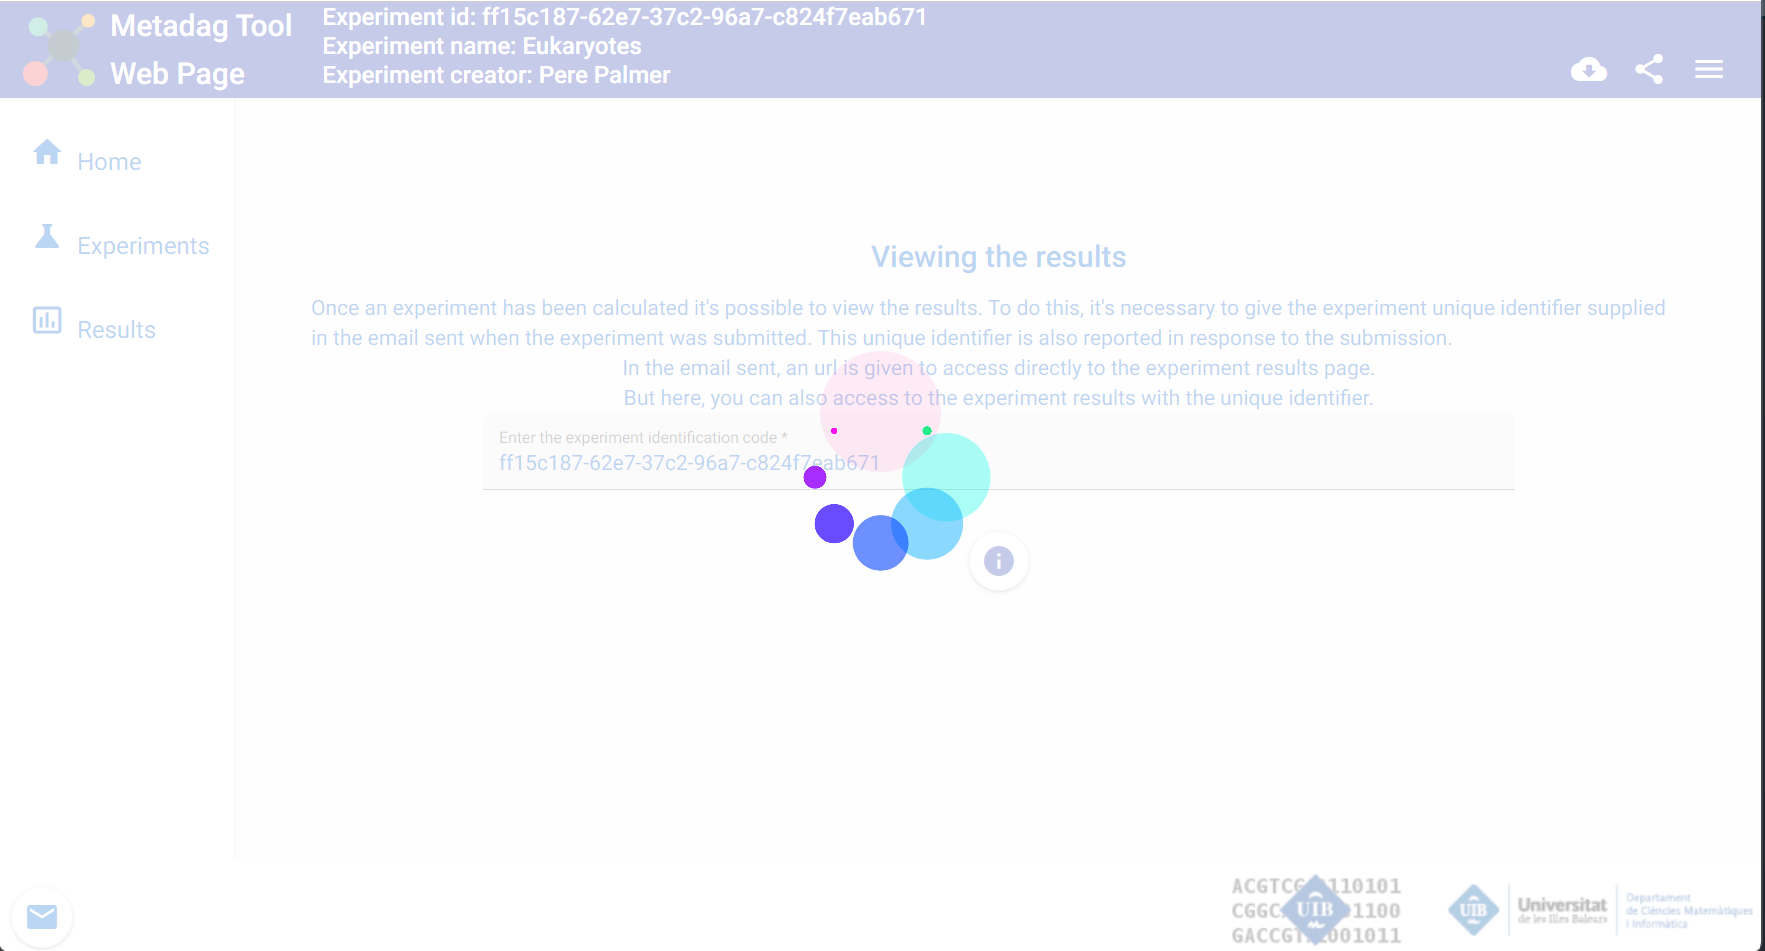
\includegraphics[width=1\textwidth,height=\textheight]{figures/screen_4.png}

\begin{Shaded}
\begin{Highlighting}[]
\NormalTok{experiment}\OtherTok{=}
  \StringTok{"result\_0a845f74{-}826e{-}3b46{-}aed9{-}e7ecf74db262/"}
\NormalTok{path\_exp}\OtherTok{=}\FunctionTok{paste0}\NormalTok{(}\StringTok{"data/"}\NormalTok{,experiment)}
\NormalTok{knitr}\SpecialCharTok{::}\FunctionTok{kable}\NormalTok{(}\FunctionTok{data.frame}\NormalTok{(}
  \AttributeTok{Directory\_files\_and\_folders=}\FunctionTok{dir}\NormalTok{(path\_exp),}
  \AttributeTok{Type=}\FunctionTok{c}\NormalTok{(}\FunctionTok{rep}\NormalTok{(}\StringTok{"Data file"}\NormalTok{,}\DecValTok{2}\NormalTok{),}
  \FunctionTok{rep}\NormalTok{(}\StringTok{"Directory"}\NormalTok{,}\DecValTok{3}\NormalTok{),}
  \FunctionTok{rep}\NormalTok{(}\StringTok{"Data file"}\NormalTok{,}\DecValTok{6}\NormalTok{),}
  \StringTok{"Directory"}\NormalTok{)))}
\end{Highlighting}
\end{Shaded}

\begin{tabular}{l|l}
\hline
Directory\_files\_and\_folders & Type\\
\hline
Different\_MBB.csv & Data file\\
\hline
Different\_mDAG.csv & Data file\\
\hline
Global & Directory\\
\hline
Groups & Directory\\
\hline
Individuals & Directory\\
\hline
Report.pdf & Data file\\
\hline
Results.csv & Data file\\
\hline
Similarities\_MBB\_MSAMethod.csv & Data file\\
\hline
Similarities\_MBB\_MunkresMethod.csv & Data file\\
\hline
Similarities\_mDAG\_MSAMethod.csv & Data file\\
\hline
Similarities\_mDAG\_MunkresMethod.csv & Data file\\
\hline
TaxonomyLevels & Directory\\
\hline
\end{tabular}

\begin{Shaded}
\begin{Highlighting}[]
\NormalTok{MBB}\OtherTok{=}\FunctionTok{read\_csv}\NormalTok{(}\FunctionTok{paste0}\NormalTok{(path\_exp,}\StringTok{"Different\_MBB.csv"}\NormalTok{),}
             \AttributeTok{show\_col\_types =} \ConstantTok{FALSE}\NormalTok{)}
\NormalTok{mDAG}\OtherTok{=}\FunctionTok{read\_csv}\NormalTok{(}\FunctionTok{paste0}\NormalTok{(path\_exp,}\StringTok{"Different\_mDAG.csv"}\NormalTok{),}
              \AttributeTok{show\_col\_types =} \ConstantTok{FALSE}\NormalTok{)}
\end{Highlighting}
\end{Shaded}

\hypertarget{load-metadata}{%
\section{Load metadata}\label{load-metadata}}

Organisms are sorted by Kingdom, Phylum and Class:

\begin{Shaded}
\begin{Highlighting}[]
\NormalTok{path\_exp}
\end{Highlighting}
\end{Shaded}

\begin{verbatim}
[1] "data/result_0a845f74-826e-3b46-aed9-e7ecf74db262/"
\end{verbatim}

\begin{Shaded}
\begin{Highlighting}[]
\NormalTok{Results}\OtherTok{=}\FunctionTok{read\_csv}\NormalTok{(}\FunctionTok{paste0}\NormalTok{(path\_exp,}\StringTok{"Results.csv"}\NormalTok{))}
\CommentTok{\#rename MetaDaG variables}
\FunctionTok{names}\NormalTok{(Results)[}\FunctionTok{c}\NormalTok{(}\DecValTok{1}\NormalTok{,}\DecValTok{2}\NormalTok{,}\DecValTok{3}\NormalTok{,}\DecValTok{4}\NormalTok{,}\DecValTok{5}\NormalTok{)]}\OtherTok{=}\FunctionTok{c}\NormalTok{(}\StringTok{"Organism"}\NormalTok{,}\StringTok{"Categories"}\NormalTok{,}\StringTok{"Groups"}\NormalTok{,}\StringTok{"mDAG\_Id"}\NormalTok{,}\StringTok{"Full\_Name"}\NormalTok{)}
\NormalTok{taxo}\OtherTok{=}\NormalTok{Results }\SpecialCharTok{\%\textgreater{}\%} \FunctionTok{select}\NormalTok{(Organism}\SpecialCharTok{:}\NormalTok{Full\_Name)}
\NormalTok{taxo}\OtherTok{=}\NormalTok{taxo }\SpecialCharTok{\%\textgreater{}\%} \FunctionTok{separate}\NormalTok{(Categories,}\AttributeTok{into=}\FunctionTok{c}\NormalTok{(}\StringTok{"Kingdom"}\NormalTok{,}\StringTok{"Phylum"}\NormalTok{,}\StringTok{"Class"}\NormalTok{))}
\NormalTok{index}\OtherTok{=}\FunctionTok{which}\NormalTok{(}\FunctionTok{is.na}\NormalTok{(taxo}\SpecialCharTok{$}\NormalTok{Class))}
\NormalTok{taxo}\SpecialCharTok{$}\NormalTok{Class[index]}\OtherTok{=}\FunctionTok{paste}\NormalTok{(taxo}\SpecialCharTok{$}\NormalTok{Phylum[index])}
\NormalTok{meta\_taxo}\OtherTok{=}\NormalTok{taxo}
\NormalTok{aux}\OtherTok{=}\FunctionTok{table}\NormalTok{(meta\_taxo}\SpecialCharTok{$}\NormalTok{Phylum)}
\NormalTok{Freq\_Phylum}\OtherTok{=}\FunctionTok{tibble}\NormalTok{(}\AttributeTok{Phylum=}\FunctionTok{names}\NormalTok{(aux),}\AttributeTok{Freq\_Phylum=}\NormalTok{aux)}
\FunctionTok{names}\NormalTok{(Freq\_Phylum)}\OtherTok{=}\FunctionTok{c}\NormalTok{(}\StringTok{"Phylum"}\NormalTok{,}\StringTok{"Freq\_Phylum"}\NormalTok{)}
\NormalTok{aux}\OtherTok{=}\FunctionTok{table}\NormalTok{(meta\_taxo}\SpecialCharTok{$}\NormalTok{Class)}
\NormalTok{Freq\_Class}\OtherTok{=}\FunctionTok{tibble}\NormalTok{(}\AttributeTok{Class=}\FunctionTok{names}\NormalTok{(aux),}\AttributeTok{Freq\_Class=}\NormalTok{aux)}
\FunctionTok{names}\NormalTok{(Freq\_Class)}\OtherTok{=}\FunctionTok{c}\NormalTok{(}\StringTok{"Class"}\NormalTok{,}\StringTok{"Freq\_Class"}\NormalTok{)}


\NormalTok{meta\_taxo }\OtherTok{=}\NormalTok{ meta\_taxo }\SpecialCharTok{\%\textgreater{}\%} 
  \FunctionTok{left\_join}\NormalTok{(Freq\_Phylum) }\SpecialCharTok{\%\textgreater{}\%}
  \FunctionTok{left\_join}\NormalTok{(Freq\_Class)}
\NormalTok{meta\_taxo }\OtherTok{=}\NormalTok{ meta\_taxo }\SpecialCharTok{\%\textgreater{}\%} 
  \FunctionTok{arrange}\NormalTok{(Kingdom,}\FunctionTok{desc}\NormalTok{(Freq\_Phylum),Phylum,}
          \FunctionTok{desc}\NormalTok{(Freq\_Class),Class)}
\FunctionTok{head}\NormalTok{(meta\_taxo)}
\end{Highlighting}
\end{Shaded}

\begin{verbatim}
# A tibble: 6 x 9
  Organism Kingdom Phylum  Class Groups mDAG_Id Full_Name Freq_Phylum Freq_Class
  <chr>    <chr>   <chr>   <chr> <chr>  <chr>   <chr>     <table[1d]> <table[1d>
1 aamp     Animals Verteb~ Mamm~ Clust~ 0313    Arvicola~ 331         139       
2 afz      Animals Verteb~ Mamm~ Clust~ 0143    Antechin~ 331         139       
3 ajm      Animals Verteb~ Mamm~ Clust~ 0221    Artibeus~ 331         139       
4 aju      Animals Verteb~ Mamm~ Clust~ 0224    Acinonyx~ 331         139       
5 aml      Animals Verteb~ Mamm~ Clust~ 0279    Ailuropo~ 331         139       
6 anu      Animals Verteb~ Mamm~ Clust~ 0310    Arvicant~ 331         139       
\end{verbatim}

\begin{Shaded}
\begin{Highlighting}[]
\FunctionTok{table}\NormalTok{(meta\_taxo}\SpecialCharTok{$}\NormalTok{Kingdom) }\SpecialCharTok{\%\textgreater{}\%}\NormalTok{ kable }\SpecialCharTok{\%\textgreater{}\%}
  \FunctionTok{kable\_styling}\NormalTok{(}\StringTok{"striped"}\NormalTok{, }\AttributeTok{full\_width =}\NormalTok{ F,}\AttributeTok{position=}\StringTok{"left"}\NormalTok{)}\SpecialCharTok{\%\textgreater{}\%} 
 \FunctionTok{scroll\_box}\NormalTok{(}\AttributeTok{width =} \StringTok{"400px"}\NormalTok{, }\AttributeTok{height =} \StringTok{"200px"}\NormalTok{)}
\end{Highlighting}
\end{Shaded}

\begin{tabular}{l|r}
\hline
Var1 & Freq\\
\hline
Animals & 535\\
\hline
Fungi & 154\\
\hline
Plants & 139\\
\hline
Protists & 56\\
\hline
\end{tabular}

\begin{Shaded}
\begin{Highlighting}[]
\FunctionTok{table}\NormalTok{(meta\_taxo}\SpecialCharTok{$}\NormalTok{Phylum,meta\_taxo}\SpecialCharTok{$}\NormalTok{Kingdom) }\SpecialCharTok{\%\textgreater{}\%}\NormalTok{ kable }\SpecialCharTok{\%\textgreater{}\%}
  \FunctionTok{kable\_styling}\NormalTok{(}\StringTok{"striped"}\NormalTok{, }\AttributeTok{full\_width =}\NormalTok{ F,}\AttributeTok{position=}\StringTok{"left"}\NormalTok{)}\SpecialCharTok{\%\textgreater{}\%} 
 \FunctionTok{scroll\_box}\NormalTok{(}\AttributeTok{width =} \StringTok{"500px"}\NormalTok{, }\AttributeTok{height =} \StringTok{"500px"}\NormalTok{)}
\end{Highlighting}
\end{Shaded}

\begin{tabular}{l|r|r|r|r}
\hline
  & Animals & Fungi & Plants & Protists\\
\hline
Alveolates & 0 & 0 & 0 & 25\\
\hline
Amoebozoa & 0 & 0 & 0 & 7\\
\hline
Annelids & 1 & 0 & 0 & 0\\
\hline
Arthropods & 158 & 0 & 0 & 0\\
\hline
Ascomycetes & 0 & 113 & 0 & 0\\
\hline
Basal & 0 & 0 & 2 & 0\\
\hline
Basidiomycetes & 0 & 36 & 0 & 0\\
\hline
Brachiopodas & 1 & 0 & 0 & 0\\
\hline
Cephalochordates & 2 & 0 & 0 & 0\\
\hline
Choanoflagellates & 0 & 0 & 0 & 2\\
\hline
Cnidarians & 10 & 0 & 0 & 0\\
\hline
Cryptomonads & 0 & 0 & 0 & 1\\
\hline
Echinoderms & 3 & 0 & 0 & 0\\
\hline
Eudicots & 0 & 0 & 98 & 0\\
\hline
Euglenozoa & 0 & 0 & 0 & 9\\
\hline
Ferns & 0 & 0 & 1 & 0\\
\hline
Flatworms & 4 & 0 & 0 & 0\\
\hline
Green & 0 & 0 & 11 & 0\\
\hline
Haptophyta & 0 & 0 & 0 & 1\\
\hline
Hemichordates & 1 & 0 & 0 & 0\\
\hline
Heterolobosea & 0 & 0 & 0 & 1\\
\hline
Metamonada & 0 & 0 & 0 & 2\\
\hline
Microsporidians & 0 & 5 & 0 & 0\\
\hline
Mollusks & 14 & 0 & 0 & 0\\
\hline
Monocots & 0 & 0 & 23 & 0\\
\hline
Mosses & 0 & 0 & 1 & 0\\
\hline
Nematodes & 6 & 0 & 0 & 0\\
\hline
Placozoans & 1 & 0 & 0 & 0\\
\hline
Poriferans & 1 & 0 & 0 & 0\\
\hline
Red & 0 & 0 & 3 & 0\\
\hline
Stramenopiles & 0 & 0 & 0 & 8\\
\hline
Tunicates & 2 & 0 & 0 & 0\\
\hline
Vertebrates & 331 & 0 & 0 & 0\\
\hline
\end{tabular}

\hypertarget{table-of-mbbs}{%
\section{Table of MBBs}\label{table-of-mbbs}}

In this example \texttt{MBB} is a table with 5149 rows and 4122 columns.
It displays, for every MBB, the selected groups (Kingdoms, families,
etc.) to which it belongs.

\begin{Shaded}
\begin{Highlighting}[]
\CommentTok{\#100}
\NormalTok{knitr}\SpecialCharTok{::}\FunctionTok{kable}\NormalTok{(MBB[}\DecValTok{1}\SpecialCharTok{:}\DecValTok{20}\NormalTok{,}\DecValTok{1}\SpecialCharTok{:}\DecValTok{10}\NormalTok{]) }\SpecialCharTok{\%\textgreater{}\%}   
  \FunctionTok{scroll\_box}\NormalTok{(}\AttributeTok{width =} \StringTok{"100\%"}\NormalTok{, }\AttributeTok{height =} \StringTok{"200px"}\NormalTok{)}
\end{Highlighting}
\end{Shaded}

\begin{tabular}{l|r|r|r|r|r|r|r|r|r}
\hline
MBB Id & natural & \#pathways & Protists & Fungi & Plants & Animals & Alveolates & Amoebozoa & Annelids\\
\hline
0 & 0 & 0 & 0 & 0 & 0 & 0 & 0 & 0 & 0\\
\hline
0.0 & 0 & 0 & 0 & 0 & 0 & 0 & 0 & 0 & 0\\
\hline
0.0.0 & 0 & 0 & 0 & 0 & 0 & 0 & 0 & 0 & 0\\
\hline
0.0.0.0 & 1 & 1 & 0 & 0 & 0 & 1 & 0 & 0 & 0\\
\hline
0.0.0.0.0 & 1 & 1 & 0 & 0 & 0 & 1 & 0 & 0 & 0\\
\hline
0.0.0.0.0.0 & 1 & 1 & 0 & 0 & 0 & 1 & 0 & 0 & 0\\
\hline
0.0.0.1 & 1 & 1 & 0 & 0 & 0 & 1 & 0 & 0 & 0\\
\hline
0.0.0.2 & 1 & 1 & 0 & 0 & 0 & 1 & 0 & 0 & 0\\
\hline
0.0.1 & 0 & 0 & 0 & 0 & 0 & 0 & 0 & 0 & 0\\
\hline
0.0.1.0 & 1 & 1 & 0 & 0 & 0 & 1 & 0 & 0 & 1\\
\hline
0.0.1.1 & 1 & 1 & 1 & 0 & 0 & 0 & 0 & 0 & 0\\
\hline
0.0.1.1.0 & 1 & 1 & 1 & 0 & 0 & 0 & 0 & 0 & 0\\
\hline
0.0.1.2 & 1 & 1 & 0 & 0 & 0 & 1 & 0 & 0 & 0\\
\hline
0.0.1.3 & 1 & 1 & 0 & 0 & 0 & 1 & 0 & 0 & 0\\
\hline
0.0.1.4 & 1 & 1 & 0 & 0 & 0 & 1 & 0 & 0 & 0\\
\hline
0.0.1.4.0 & 1 & 1 & 0 & 0 & 0 & 1 & 0 & 0 & 0\\
\hline
0.0.1.4.0.0 & 1 & 1 & 0 & 0 & 0 & 1 & 0 & 0 & 0\\
\hline
0.0.1.5 & 1 & 1 & 1 & 0 & 0 & 0 & 0 & 0 & 0\\
\hline
0.0.1.6 & 1 & 4 & 3 & 0 & 0 & 1 & 0 & 0 & 0\\
\hline
0.0.1.6.0 & 1 & 3 & 0 & 0 & 3 & 0 & 0 & 0 & 0\\
\hline
\end{tabular}

\hypertarget{table-of-m-dags}{%
\section{Table of m-DAGs}\label{table-of-m-dags}}

In this example \texttt{mDAG} is a table with 1132 rows and 5278
columns. It displays, for every m-DAG, the selected groups (Kingdoms,
families, etc.) in which it belongs.

\begin{Shaded}
\begin{Highlighting}[]
\FunctionTok{kable}\NormalTok{(mDAG[}\DecValTok{1}\SpecialCharTok{:}\DecValTok{20}\NormalTok{,}\DecValTok{1}\SpecialCharTok{:}\DecValTok{10}\NormalTok{]) }\SpecialCharTok{\%\textgreater{}\%}   \FunctionTok{scroll\_box}\NormalTok{(}\AttributeTok{width =} \StringTok{"100\%"}\NormalTok{, }\AttributeTok{height =} \StringTok{"200px"}\NormalTok{)}
\end{Highlighting}
\end{Shaded}

\begin{tabular}{l|r|r|r|r|r|r|r|r|r}
\hline
mDAG Id & \#Categories & Animals & Plants & Fungi & Protists & Alveolates & Amoebozoa & Annelids & Arthropods\\
\hline
0001 & 3 & 1 & 0 & 0 & 0 & 0 & 0 & 0 & 0\\
\hline
0002 & 2 & 0 & 0 & 1 & 0 & 0 & 0 & 0 & 0\\
\hline
0003 & 2 & 1 & 0 & 0 & 0 & 0 & 0 & 0 & 0\\
\hline
0004 & 3 & 1 & 0 & 0 & 0 & 0 & 0 & 0 & 0\\
\hline
0005 & 3 & 1 & 0 & 0 & 0 & 0 & 0 & 0 & 0\\
\hline
0006 & 3 & 0 & 1 & 0 & 0 & 0 & 0 & 0 & 0\\
\hline
0007 & 2 & 0 & 1 & 0 & 0 & 0 & 0 & 0 & 0\\
\hline
0008 & 3 & 0 & 1 & 0 & 0 & 0 & 0 & 0 & 0\\
\hline
0009 & 3 & 0 & 1 & 0 & 0 & 0 & 0 & 0 & 0\\
\hline
0010 & 3 & 1 & 0 & 0 & 0 & 0 & 0 & 0 & 0\\
\hline
0011 & 3 & 1 & 0 & 0 & 0 & 0 & 0 & 0 & 0\\
\hline
0012 & 3 & 0 & 0 & 0 & 1 & 0 & 0 & 0 & 0\\
\hline
0013 & 3 & 1 & 0 & 0 & 0 & 0 & 0 & 0 & 0\\
\hline
0014 & 3 & 0 & 0 & 0 & 1 & 1 & 0 & 0 & 0\\
\hline
0015 & 2 & 0 & 0 & 1 & 0 & 0 & 0 & 0 & 0\\
\hline
0016 & 3 & 0 & 0 & 0 & 1 & 0 & 1 & 0 & 0\\
\hline
0017 & 3 & 1 & 0 & 0 & 0 & 0 & 0 & 0 & 0\\
\hline
0018 & 3 & 1 & 0 & 0 & 0 & 0 & 0 & 0 & 0\\
\hline
0019 & 3 & 1 & 0 & 0 & 0 & 0 & 0 & 0 & 1\\
\hline
0020 & 3 & 1 & 0 & 0 & 0 & 0 & 0 & 0 & 0\\
\hline
\end{tabular}

\begin{Shaded}
\begin{Highlighting}[]
\FunctionTok{dim}\NormalTok{(mDAG)}
\end{Highlighting}
\end{Shaded}

\begin{verbatim}
[1] 1132 5278
\end{verbatim}

\begin{Shaded}
\begin{Highlighting}[]
\FunctionTok{names}\NormalTok{(mDAG)[}\DecValTok{1}\SpecialCharTok{:}\DecValTok{6}\NormalTok{]}
\end{Highlighting}
\end{Shaded}

\begin{verbatim}
[1] "mDAG Id"     "#Categories" "Animals"     "Plants"      "Fungi"      
[6] "Protists"   
\end{verbatim}

\begin{Shaded}
\begin{Highlighting}[]
\FunctionTok{head}\NormalTok{(}\FunctionTok{names}\NormalTok{(mDAG)[}\DecValTok{7}\SpecialCharTok{:}\NormalTok{(}\FunctionTok{dim}\NormalTok{(mDAG)[}\DecValTok{2}\NormalTok{]}\SpecialCharTok{{-}}\DecValTok{1150}\NormalTok{)])}
\end{Highlighting}
\end{Shaded}

\begin{verbatim}
[1] "Alveolates"        "Amoebozoa"         "Annelids"         
[4] "Arthropods"        "Ascomycetes"       "Basal angiosperms"
\end{verbatim}

\begin{Shaded}
\begin{Highlighting}[]
\CommentTok{\# 28 to 1213  code MBB: 1 if MBB in mDAG 0}
\end{Highlighting}
\end{Shaded}

\hypertarget{results-table}{%
\section{Results Table}\label{results-table}}

The \texttt{Results} table contains for every organism (row) the
following information: its category (taxonomy), selected group, Full
name, m-DAG id and all reactions name id with their corresponding
enzyme. When a reaction is present in the corresponding m-DAG, the MBB
to which it belongs is displayed in this column.

\begin{Shaded}
\begin{Highlighting}[]
\FunctionTok{kable}\NormalTok{(Results[}\DecValTok{1}\SpecialCharTok{:}\DecValTok{20}\NormalTok{,}\DecValTok{1}\SpecialCharTok{:}\DecValTok{10}\NormalTok{])}\SpecialCharTok{\%\textgreater{}\%}
  \FunctionTok{row\_spec}\NormalTok{(}\DecValTok{0}\NormalTok{, }\AttributeTok{angle =} \DecValTok{0}\NormalTok{) }\SpecialCharTok{\%\textgreater{}\%}   
  \FunctionTok{scroll\_box}\NormalTok{(}\AttributeTok{width =} \StringTok{"300\%"}\NormalTok{, }\AttributeTok{height =} \StringTok{"1000px"}\NormalTok{)}
\end{Highlighting}
\end{Shaded}

\begin{tabular}{l|l|l|l|l|l|r|l|l|l}
\hline
\rotatebox{0}{Organism} & \rotatebox{0}{Categories} & \rotatebox{0}{Groups} & \rotatebox{0}{mDAG\_Id} & \rotatebox{0}{Full\_Name} & \rotatebox{0}{R00005(3.5.1.54)} & \rotatebox{0}{R00009(1.11.1.6)} & \rotatebox{0}{R00010(3.2.1.28)} & \rotatebox{0}{R00014(1.2.4.1)} & \rotatebox{0}{R00014(4.1.1.1)}\\
\hline
aaf & Protists|Stramenopiles|Pelagophytes & MSA Cluster 3|MUN Cluster 3 & 0036 & Aureococcus anophagefferens & NA & NA & 0.0.10.0.15 & 0.0.10.0.15 & NA\\
\hline
aag & Animals|Arthropods|Insects & MSA Cluster 2|MUN Cluster 2 & 0035 & Aedes aegypti (yellow fever mosquito) & NA & 3936 & 0.9.27.7.36.14 & 0.9.27.7.36.14 & NA\\
\hline
aalb & Animals|Arthropods|Insects & MSA Cluster 2|MUN Cluster 2 & 0276 & Aedes albopictus (Asian tiger mosquito) & NA & 3936 & 0.9.27.7.36.18 & 0.9.27.7.36.18 & NA\\
\hline
aali & Animals|Arthropods|Insects & MSA Cluster 2|MUN Cluster 2 & 0267 & Anopheles albimanus & NA & 3936 & 0.9.27.7.36.65 & 0.9.27.7.36.65 & NA\\
\hline
aalt & Fungi|Ascomycetes|Dothideomycetes & Fungui and Algae|MSA Cluster 3|MSA Fungui and Nematodes and Flatworms|MUN Cluster 3|MUN Fungui and Nematodes and Flatworms & 0240 & Alternaria alternata & NA & 3936 & 0.0.9.20.0.5.6.7 & 0.0.9.20.0.5.6.7 & 0.0.9.20.0.5.6.7\\
\hline
aam & Animals|Vertebrates|Birds & Cluster 1 & 0040 & Apteryx mantelli mantelli (North Island brown kiwi) & NA & 3936 & NA & 0.9.26.15.46 & NA\\
\hline
aamp & Animals|Vertebrates|Mammals & Cluster 1 & 0313 & Arvicola amphibius (Eurasian water vole) & NA & 3936 & 0.0.9.20.0.6.0.39 & 0.9.26.18.2.0 & NA\\
\hline
aang & Animals|Vertebrates|Fishes & Cluster 1 & 0317 & Anguilla anguilla (European eel) & NA & 3936 & 0.0.9.20.0.6.0.39 & 0.9.26.17.0.0 & NA\\
\hline
aara & Animals|Arthropods|Insects & MSA Cluster 2|MUN Cluster 2 & 0362 & Anopheles arabiensis & NA & 3936 & 0.9.27.7.36.34 & 0.9.27.7.36.34 & NA\\
\hline
abe & Fungi|Ascomycetes|Eurotiomycetes & Fungui and Algae|MSA Cluster 3|MSA Fungui and Nematodes and Flatworms|MUN Cluster 3|MUN Fungui and Nematodes and Flatworms & 0060 & Trichophyton benhamiae & NA & 3936 & 0.0.9.20.0.5.7.0 & 0.0.9.20.0.5.7.0 & 0.0.9.20.0.5.7.0\\
\hline
abp & Fungi|Basidiomycetes & Fungui and Algae|MSA Cluster 3|MSA Fungui and Nematodes and Flatworms|MUN Cluster 3|MUN Fungui and Nematodes and Flatworms & 0068 & Agaricus bisporus var. burnettii JB137-S8 & NA & 3936 & 0.0.9.20.0.6.1 & 0.0.9.20.0.6.1 & 0.0.9.20.0.6.1\\
\hline
abv & Fungi|Basidiomycetes & Fungui and Algae|MSA Cluster 3|MSA Fungui and Nematodes and Flatworms|MUN Cluster 3|MUN Fungui and Nematodes and Flatworms & 0073 & Agaricus bisporus var. bisporus H97 & NA & 3936 & 0.0.9.20.0.6.3 & 0.0.9.20.0.6.3 & 0.0.9.20.0.6.3\\
\hline
acan & Protists|Amoebozoa|Acanthamoeba & MSA Cluster 3|MUN Cluster 3 & 0873 & Acanthamoeba castellanii & NA & 3936 & NA & 0.0.10.0.3 & NA\\
\hline
acar & Animals|Vertebrates|Birds & Cluster 1 & 0884 & Antrostomus carolinensis (chuck-will's-widow) & NA & 3936 & NA & 0.9.26.15.59 & NA\\
\hline
acep & Animals|Arthropods|Insects & MSA Cluster 2|MUN Cluster 2 & 0054 & Atta cephalotes (leaf cutting ant) & NA & 3936 & 0.9.27.7.36.56 & 0.9.27.7.36.56 & NA\\
\hline
acer & Animals|Arthropods|Insects & MSA Cluster 2|MUN Cluster 2 & 0057 & Apis cerana (Asiatic honeybee) & NA & 3936 & 0.9.27.7.35.34 & 0.9.27.7.35.34 & NA\\
\hline
achc & Animals|Vertebrates|Birds & Cluster 1 & 0103 & Aquila chrysaetos chrysaetos (golden eagle) & NA & 3936 & NA & 0.9.26.15.2.0 & NA\\
\hline
ache & Fungi|Ascomycetes|Eurotiomycetes & Fungui and Algae|MSA Cluster 3|MSA Fungui and Nematodes and Flatworms|MUN Cluster 3|MUN Fungui and Nematodes and Flatworms & 0106 & Aspergillus chevalieri & NA & 3936 & 0.0.9.20.0.5.7.2 & 0.0.9.20.0.5.7.2 & 0.0.9.20.0.5.7.2\\
\hline
achl & Animals|Vertebrates|Birds & Cluster 1 & 0081 & Acanthisitta chloris (rifleman) & NA & 3936 & NA & 0.9.26.15.1.1.0.0 & NA\\
\hline
acoz & Animals|Arthropods|Insects & MSA Cluster 2|MUN Cluster 2 & 0255 & Anopheles coluzzii & NA & 3936 & 0.9.27.7.36.22 & 0.9.27.7.36.22 & NA\\
\hline
\end{tabular}

\begin{Shaded}
\begin{Highlighting}[]
\FunctionTok{dim}\NormalTok{(Results)}
\end{Highlighting}
\end{Shaded}

\begin{verbatim}
[1] 1132 3998
\end{verbatim}

\begin{Shaded}
\begin{Highlighting}[]
\FunctionTok{names}\NormalTok{(Results)[}\DecValTok{1}\NormalTok{]}\CommentTok{\# organisms  kegg id  class representant of mDAG}
\end{Highlighting}
\end{Shaded}

\begin{verbatim}
[1] "Organism"
\end{verbatim}

\begin{Shaded}
\begin{Highlighting}[]
\FunctionTok{names}\NormalTok{(Results)[}\DecValTok{2}\NormalTok{]}\CommentTok{\# taxonomy separate by |}
\end{Highlighting}
\end{Shaded}

\begin{verbatim}
[1] "Categories"
\end{verbatim}

\begin{Shaded}
\begin{Highlighting}[]
\FunctionTok{names}\NormalTok{(Results)[}\DecValTok{3}\NormalTok{]}\CommentTok{\# groups }
\end{Highlighting}
\end{Shaded}

\begin{verbatim}
[1] "Groups"
\end{verbatim}

\begin{Shaded}
\begin{Highlighting}[]
\FunctionTok{names}\NormalTok{(Results)[}\DecValTok{4}\NormalTok{]}\CommentTok{\# mDAG\_Id }
\end{Highlighting}
\end{Shaded}

\begin{verbatim}
[1] "mDAG_Id"
\end{verbatim}

\begin{Shaded}
\begin{Highlighting}[]
\FunctionTok{names}\NormalTok{(Results)[}\DecValTok{5}\NormalTok{]}\CommentTok{\# Full name representant}
\end{Highlighting}
\end{Shaded}

\begin{verbatim}
[1] "Full_Name"
\end{verbatim}

\begin{Shaded}
\begin{Highlighting}[]
\FunctionTok{names}\NormalTok{(Results)[}\DecValTok{6}\SpecialCharTok{:}\DecValTok{36}\NormalTok{]}\CommentTok{\# columns 6 to 3998 }
\end{Highlighting}
\end{Shaded}

\begin{verbatim}
 [1] "R00005(3.5.1.54)"   "R00009(1.11.1.6)"   "R00010(3.2.1.28)"  
 [4] "R00014(1.2.4.1)"    "R00014(4.1.1.1)"    "R00021(1.4.7.1)"   
 [7] "R00022(3.2.1.52)"   "R00024(4.1.1.39)"   "R00028(3.2.1.20)"  
[10] "R00031(1.10.3.1)"   "R00032(1.13.11.63)" "R00036(4.2.1.24)"  
[13] "R00045(1.10.3.1)"   "R00066(2.5.1.9)"    "R00068(1.10.3.3)"  
[16] "R00073(1.14.99.1)"  "R00075(2.5.1.43)"   "R00078(1.16.3.1)"  
[19] "R00084(2.5.1.61)"   "R00086(3.6.1.15)"   "R00086(3.6.1.5)"   
[22] "R00087(3.6.1.9)"    "R00093(1.4.1.14)"   "R00095(1.6.5.4)"   
[25] "R00100(1.6.2.2)"    "R00102(3.2.2.5)"    "R00102(3.2.2.6)"   
[28] "R00103(3.6.1.22)"   "R00103(3.6.1.9)"    "R00104(2.7.1.23)"  
[31] "R00111(1.14.13.39)"
\end{verbatim}

\begin{Shaded}
\begin{Highlighting}[]
\CommentTok{\# reactions name id with its enzyme.}
\end{Highlighting}
\end{Shaded}

\begin{Shaded}
\begin{Highlighting}[]
\NormalTok{reactions}\OtherTok{=}\FunctionTok{names}\NormalTok{(Results)[}\SpecialCharTok{{-}}\FunctionTok{c}\NormalTok{(}\DecValTok{1}\SpecialCharTok{:}\DecValTok{5}\NormalTok{)]}
\NormalTok{reverse\_reactions}\OtherTok{=}\NormalTok{stringr}\SpecialCharTok{::}\FunctionTok{str\_detect}\NormalTok{(reactions,}\StringTok{"rev"}\NormalTok{)}
\NormalTok{reverse\_reactions}\OtherTok{=}\FunctionTok{table}\NormalTok{(reverse\_reactions)}
\FunctionTok{dimnames}\NormalTok{(reverse\_reactions)}\SpecialCharTok{$}\NormalTok{reverse\_reactions}\OtherTok{=}
  \FunctionTok{c}\NormalTok{(}\StringTok{"Non reverse reaction"}\NormalTok{,}\StringTok{"Reverse reaction"}\NormalTok{)}
\NormalTok{reverse\_reactions}
\end{Highlighting}
\end{Shaded}

\begin{verbatim}
reverse_reactions
Non reverse reaction     Reverse reaction 
                3399                  594 
\end{verbatim}

\bookmarksetup{startatroot}

\hypertarget{metabolic-graphs}{%
\chapter{Metabolic Graphs}\label{metabolic-graphs}}

We present here some analysis examples of the metabolic graphs generated
in GraphML format.

\hypertarget{metabolic-graphs-for-each-organism}{%
\section{Metabolic graphs for each
organism}\label{metabolic-graphs-for-each-organism}}

Read the individual metabolic graphs generated for Homo sapiens (KEGG
id: hsa) in the directory(Individuals/hsa)

\begin{Shaded}
\begin{Highlighting}[]
\NormalTok{files\_hsa}\OtherTok{=}\FunctionTok{dir}\NormalTok{(}\FunctionTok{paste0}\NormalTok{(path\_exp,}\StringTok{"Individuals/hsa"}\NormalTok{))}
\NormalTok{files\_hsa}
\end{Highlighting}
\end{Shaded}

\begin{verbatim}
 [1] "hsa_mDAG.graphml"       "hsa_mDAG.pdf"           "hsa_mDAG.svg"          
 [4] "hsa_mDAG_adj.csv"       "hsa_mDAG_biggerDAG.pdf" "hsa_mDAG_biggerDAG.svg"
 [7] "hsa_mDAG_nl.csv"        "hsa_mDAG_structure.csv" "hsa_R_adj.csv"         
[10] "hsa_R_nl.csv"           "hsa_RC.graphml"         "hsa_RC.pdf"            
[13] "hsa_RC.svg"             "hsa_summary.txt"       
\end{verbatim}

\begin{tabular}{l|l}
\hline
files\_Individual\_hsa & Description\\
\hline
hsa\_mDAG.graphml & m-DAG GraphML format\\
\hline
hsa\_mDAG.pdf & m-DAG pdf graphic\\
\hline
hsa\_mDAG.svg & m-DAG svg graphic\\
\hline
hsa\_mDAG\_adj.csv & csv file with the adjacency matrix of the m-DAG\\
\hline
hsa\_mDAG\_biggerDAG.pdf & pdf graphic with the biggest conected componet of the m-DAG\\
\hline
hsa\_mDAG\_biggerDAG.svg & svg graphic with the biggest conected componet of the m-DAG\\
\hline
hsa\_mDAG\_nl.csv & csv file with the node (MBBs) labels  of the m-DAG\\
\hline
hsa\_mDAG\_structure.csv & csv file with all connected components of the m-DAG\\
\hline
hsa\_R\_adj.csv & csv file with the  adjacency matrix of the reaction graph\\
\hline
hsa\_R\_nl.csv & csv file with the node (reactions) labels  of the reaction graph\\
\hline
hsa\_RC.graphml & reaction graph  GraphML format\\
\hline
hsa\_RC.pdf & reaction graph pdf graphic\\
\hline
hsa\_RC.svg & reaction graph svg graphic\\
\hline
hsa\_summary.txt & text summary file with the number of MBBs, reactions, etc. in the previous graphs\\
\hline
\end{tabular}

\hypertarget{pan-core-metabolic-graphs}{%
\section{Pan \& core metabolic graphs}\label{pan-core-metabolic-graphs}}

Pan and core metabolic graphs for every group were generated. For
instance, one can read the pan and core metabolic graphs generated for
the group Algae in the directory (Groups/Algae).

\begin{Shaded}
\begin{Highlighting}[]
\NormalTok{files\_Algae}\OtherTok{=}\FunctionTok{dir}\NormalTok{(}\FunctionTok{paste0}\NormalTok{(path\_exp,}\StringTok{"Groups/Algae"}\NormalTok{))}
\NormalTok{files\_Algae}
\end{Highlighting}
\end{Shaded}

\begin{verbatim}
[1] "core" "pan" 
\end{verbatim}

The global core reaction graph, which is the core of all the organisms'
reaction graphs in this Eukaryotes test, is empty.

\begin{Shaded}
\begin{Highlighting}[]
\NormalTok{graph\_core\_RC}\OtherTok{=}\FunctionTok{read.graph}\NormalTok{(}
  \FunctionTok{paste0}\NormalTok{(path\_exp,}
         \StringTok{"Global/core/core\_RC.graphml"}\NormalTok{),}
  \AttributeTok{format =} \StringTok{"graphml"}\NormalTok{)}
\FunctionTok{summary}\NormalTok{(graph\_core\_RC)}
\end{Highlighting}
\end{Shaded}

\begin{verbatim}
IGRAPH a145f88 D--- 0 0 -- 
+ attr: color (v/c), label (v/c), id (v/c)
\end{verbatim}

The global core reaction graph has 0 vertex and 0 edges. It is an empty
graph.

The core reaction graph for the Algae group is:

\begin{Shaded}
\begin{Highlighting}[]
\NormalTok{knitr}\SpecialCharTok{::}\FunctionTok{include\_graphics}\NormalTok{(}
  \FunctionTok{paste0}\NormalTok{(path\_exp,}\StringTok{"Groups/MSA\_Cluster\_3/core/MSA\_Cluster\_3\_core\_RC.pdf"}\NormalTok{))}
\end{Highlighting}
\end{Shaded}

\begin{figure}[H]

{\centering 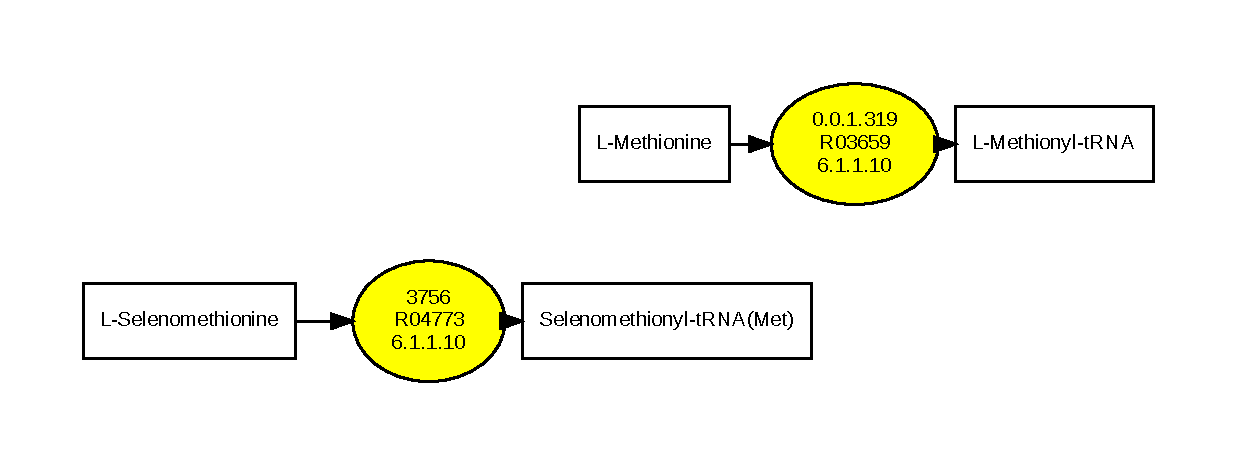
\includegraphics[width=1\textwidth,height=\textheight]{data/result_0a845f74-826e-3b46-aed9-e7ecf74db262/Groups/MSA_Cluster_3/core/MSA_Cluster_3_core_RC.pdf}

}

\caption{Algae core reaction graph}

\end{figure}

The global core m-DAG, i.e., the core of all organisms in this example
is empty.

\begin{Shaded}
\begin{Highlighting}[]
\NormalTok{graph\_core\_mDAG}\OtherTok{=}\FunctionTok{read.graph}\NormalTok{(}
  \FunctionTok{paste0}\NormalTok{(path\_exp,}\StringTok{"Global/core/core\_mDAG.graphml"}\NormalTok{),}
  \AttributeTok{format =} \StringTok{"graphml"}\NormalTok{)}
\FunctionTok{summary}\NormalTok{(graph\_core\_mDAG)}
\end{Highlighting}
\end{Shaded}

\begin{verbatim}
IGRAPH a1485a3 D--- 0 0 -- 
+ attr: color (v/c), label (v/c), id (v/c)
\end{verbatim}

The global core m-DAG has 0 vertex and 0 edges. It is an empty graph.

The core metabolic DAG for the Algae group is:

\begin{Shaded}
\begin{Highlighting}[]
\NormalTok{knitr}\SpecialCharTok{::}\FunctionTok{include\_graphics}\NormalTok{(}\FunctionTok{paste0}\NormalTok{(path\_exp,                              }\StringTok{"Groups/Algae/core/Algae\_core\_mDAG.pdf"}\NormalTok{))}
\end{Highlighting}
\end{Shaded}

\begin{figure}[H]

{\centering \includegraphics[width=1\textwidth,height=\textheight]{data/result_0a845f74-826e-3b46-aed9-e7ecf74db262/Groups/Algae/core/Algae_core_mDAG.pdf}

}

\caption{Core m-DAG for Algae}

\end{figure}

The global pan reaction graph for the Animals Kingdom is:

\begin{Shaded}
\begin{Highlighting}[]
\NormalTok{graph\_pan\_RC}\OtherTok{=}\FunctionTok{read.graph}\NormalTok{(}
  \FunctionTok{paste0}\NormalTok{(path\_exp,}
         \StringTok{"TaxonomyLevels/Kingdom/Animals/pan/Animals\_pan\_RC.graphml"}\NormalTok{),}
  \AttributeTok{format =} \StringTok{"graphml"}\NormalTok{)}
\FunctionTok{summary}\NormalTok{(graph\_pan\_RC)}
\end{Highlighting}
\end{Shaded}

\begin{verbatim}
IGRAPH a14e485 D--- 4556 5798 -- 
+ attr: color (v/c), label (v/c), id (v/c), id (e/c)
\end{verbatim}

This pan reaction graph has 4556 nodes and 5798 edges.

\hypertarget{graphs-topology}{%
\section{Graph's topology}\label{graphs-topology}}

From the GraphML files, one can extract topological information. Some
examples are as follows.

The diagram below illustrates the distribution of node degrees for an
m-DAG.

\begin{Shaded}
\begin{Highlighting}[]
\NormalTok{graph\_mDAG}\OtherTok{=}\FunctionTok{read.graph}\NormalTok{(}
  \FunctionTok{paste0}\NormalTok{(path\_exp,}
         \StringTok{"Individuals/hsa/hsa\_mDAG.graphml"}\NormalTok{),}
  \AttributeTok{format=} \StringTok{"graphml"}\NormalTok{)}
\FunctionTok{summary}\NormalTok{(graph\_mDAG)}
\end{Highlighting}
\end{Shaded}

\begin{verbatim}
IGRAPH a15058b D--- 1026 1086 -- 
+ attr: color (v/c), label (v/c), id (v/c), id (e/c)
\end{verbatim}

\begin{Shaded}
\begin{Highlighting}[]
\FunctionTok{barplot}\NormalTok{(}\FunctionTok{table}\NormalTok{(igraph}\SpecialCharTok{::}\FunctionTok{degree}\NormalTok{(graph\_mDAG,}\AttributeTok{mode=}\StringTok{"all"}\NormalTok{)),}
              \AttributeTok{ylim=}\FunctionTok{c}\NormalTok{(}\DecValTok{0}\NormalTok{,}\DecValTok{350}\NormalTok{),}\AttributeTok{col=}\StringTok{"blue"}\NormalTok{,}
              \AttributeTok{main=}\StringTok{"Frequency of Node Degrees"}\NormalTok{,}
              \AttributeTok{ylab=}\StringTok{"Frequency"}\NormalTok{,}\AttributeTok{xlab=}\StringTok{"Degree"}\NormalTok{)}
\end{Highlighting}
\end{Shaded}

\begin{figure}[H]

{\centering 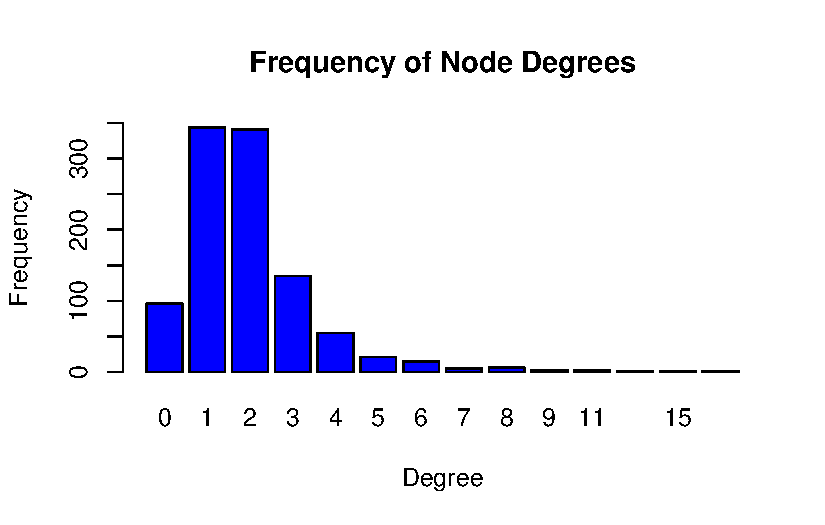
\includegraphics[width=1\textwidth,height=\textheight]{index_files/figure-pdf/unnamed-chunk-21-1.pdf}

}

\end{figure}

The connected components of every graph as well as the size of every
connected component can be obtained as:

\begin{Shaded}
\begin{Highlighting}[]
\NormalTok{compo}\OtherTok{=}\FunctionTok{components}\NormalTok{(graph\_mDAG,}\AttributeTok{mode =} \StringTok{"weak"}\NormalTok{)}
\FunctionTok{str}\NormalTok{(compo)}
\end{Highlighting}
\end{Shaded}

\begin{verbatim}
List of 3
 $ membership: num [1:1026] 1 1 1 1 1 1 1 1 1 1 ...
 $ csize     : num [1:167] 589 1 1 1 1 1 4 3 4 3 ...
 $ no        : int 167
\end{verbatim}

\begin{Shaded}
\begin{Highlighting}[]
\NormalTok{compo}\SpecialCharTok{$}\NormalTok{csize}
\end{Highlighting}
\end{Shaded}

\begin{verbatim}
  [1] 589   1   1   1   1   1   4   3   4   3   2   3   3   1   1   1   2   6
 [19]   3   1   3   6   1   1   1   1   1   3   1   6   2   1   1   1   2   1
 [37]   1  14   1  16   1   6   2   2   4   1   1   1   1   1   1   1   1   1
 [55]  13   1   1   1   1   2   6   5   5   2   2  10   1   1   1   2   2   1
 [73]   1   1  62   6   2   1   2   1   1   1   2   1   2  14   3   1   1   1
 [91]   1   1   1   1   1   1   3   6   1   3   1   3   2   1   1   1   2   2
[109]   3   1   1   2   5   1   1   2   3   2   1   1   2   3   4   1   1   2
[127]   1   1   2   1   1   1   1   1   3   1   2   2   1   6   1   1   1   2
[145]   1   1   1   1   1   2   7   1  15   3   1   1   1   1   2   1   3   1
[163]   1   1   1   1   2
\end{verbatim}

\begin{Shaded}
\begin{Highlighting}[]
\NormalTok{k}\OtherTok{=}\FunctionTok{which.max}\NormalTok{(compo}\SpecialCharTok{$}\NormalTok{csize}\SpecialCharTok{==}\FunctionTok{max}\NormalTok{(compo}\SpecialCharTok{$}\NormalTok{csize))}
\NormalTok{k}
\end{Highlighting}
\end{Shaded}

\begin{verbatim}
[1] 1
\end{verbatim}

\begin{Shaded}
\begin{Highlighting}[]
\FunctionTok{table}\NormalTok{(compo}\SpecialCharTok{$}\NormalTok{membership)}
\end{Highlighting}
\end{Shaded}

\begin{verbatim}

  1   2   3   4   5   6   7   8   9  10  11  12  13  14  15  16  17  18  19  20 
589   1   1   1   1   1   4   3   4   3   2   3   3   1   1   1   2   6   3   1 
 21  22  23  24  25  26  27  28  29  30  31  32  33  34  35  36  37  38  39  40 
  3   6   1   1   1   1   1   3   1   6   2   1   1   1   2   1   1  14   1  16 
 41  42  43  44  45  46  47  48  49  50  51  52  53  54  55  56  57  58  59  60 
  1   6   2   2   4   1   1   1   1   1   1   1   1   1  13   1   1   1   1   2 
 61  62  63  64  65  66  67  68  69  70  71  72  73  74  75  76  77  78  79  80 
  6   5   5   2   2  10   1   1   1   2   2   1   1   1  62   6   2   1   2   1 
 81  82  83  84  85  86  87  88  89  90  91  92  93  94  95  96  97  98  99 100 
  1   1   2   1   2  14   3   1   1   1   1   1   1   1   1   1   3   6   1   3 
101 102 103 104 105 106 107 108 109 110 111 112 113 114 115 116 117 118 119 120 
  1   3   2   1   1   1   2   2   3   1   1   2   5   1   1   2   3   2   1   1 
121 122 123 124 125 126 127 128 129 130 131 132 133 134 135 136 137 138 139 140 
  2   3   4   1   1   2   1   1   2   1   1   1   1   1   3   1   2   2   1   6 
141 142 143 144 145 146 147 148 149 150 151 152 153 154 155 156 157 158 159 160 
  1   1   1   2   1   1   1   1   1   2   7   1  15   3   1   1   1   1   2   1 
161 162 163 164 165 166 167 
  3   1   1   1   1   1   2 
\end{verbatim}

\begin{Shaded}
\begin{Highlighting}[]
\NormalTok{vertex}\OtherTok{=}\FunctionTok{which}\NormalTok{(compo}\SpecialCharTok{$}\NormalTok{membership}\SpecialCharTok{==}\NormalTok{k)}
\FunctionTok{length}\NormalTok{(vertex)}
\end{Highlighting}
\end{Shaded}

\begin{verbatim}
[1] 589
\end{verbatim}

\begin{Shaded}
\begin{Highlighting}[]
\NormalTok{Big\_Component}\OtherTok{=}\FunctionTok{induced\_subgraph}\NormalTok{(graph\_mDAG, }\AttributeTok{vids=}\NormalTok{vertex)}
\NormalTok{igraph}\SpecialCharTok{::}\FunctionTok{vcount}\NormalTok{(Big\_Component)}
\end{Highlighting}
\end{Shaded}

\begin{verbatim}
[1] 589
\end{verbatim}

\begin{Shaded}
\begin{Highlighting}[]
\NormalTok{igraph}\SpecialCharTok{::}\FunctionTok{ecount}\NormalTok{(Big\_Component)}
\end{Highlighting}
\end{Shaded}

\begin{verbatim}
[1] 774
\end{verbatim}

And the plot of the bigger component of the m-DAG in Homo sapiens is:

\begin{Shaded}
\begin{Highlighting}[]
\NormalTok{knitr}\SpecialCharTok{::}\FunctionTok{include\_graphics}\NormalTok{(}\FunctionTok{paste0}\NormalTok{(path\_exp,}
                    \StringTok{"Individuals/hsa/hsa\_mDAG\_biggerDAG.pdf"}\NormalTok{))}
\end{Highlighting}
\end{Shaded}

\begin{figure}[H]

{\centering \includegraphics[width=1\textwidth,height=\textheight]{data/result_0a845f74-826e-3b46-aed9-e7ecf74db262/Individuals/hsa/hsa_mDAG_biggerDAG.pdf}

}

\end{figure}

\begin{Shaded}
\begin{Highlighting}[]
\CommentTok{\#path\_exp="data/result\_bb261b6e{-}95c6{-}3e39{-}b82b{-}b68eea80e30b/data/" }
\NormalTok{list\_names}\OtherTok{=}\FunctionTok{dir}\NormalTok{(}\FunctionTok{paste0}\NormalTok{(path\_exp,}\StringTok{"Individuals/"}\NormalTok{))}
\NormalTok{list\_names}\OtherTok{=}\NormalTok{ list\_names[}\SpecialCharTok{{-}}\DecValTok{1}\NormalTok{] }\CommentTok{\# filter 0000\_RefPw}
\FunctionTok{length}\NormalTok{(list\_names) }
\end{Highlighting}
\end{Shaded}

\begin{verbatim}
[1] 884
\end{verbatim}

\begin{Shaded}
\begin{Highlighting}[]
\NormalTok{graphs\_list}\OtherTok{=}\FunctionTok{paste0}\NormalTok{(path\_exp,}\StringTok{"Individuals/"}\NormalTok{, list\_names,}\StringTok{"/"}\NormalTok{,list\_names, }\StringTok{"\_MDAG.graphml"}\NormalTok{)}
\end{Highlighting}
\end{Shaded}

\begin{Shaded}
\begin{Highlighting}[]
\NormalTok{knitr}\SpecialCharTok{::}\FunctionTok{include\_graphics}\NormalTok{(}
\FunctionTok{paste0}\NormalTok{(path\_exp,}\StringTok{"Individuals/cang/cang\_RC.pdf"}\NormalTok{))}
\end{Highlighting}
\end{Shaded}

\begin{figure}[H]

{\centering \includegraphics[width=1\textwidth,height=\textheight]{data/result_0a845f74-826e-3b46-aed9-e7ecf74db262/Individuals/cang/cang_RC.pdf}

}

\end{figure}

\hypertarget{graph-statistics}{%
\section{Graph statistics}\label{graph-statistics}}

The number of connected component in each generated m-DAG with their
frequency in the entire set of m-DAGs, can be obtained as follows:

\begin{Shaded}
\begin{Highlighting}[]
\NormalTok{read\_mDAG}\OtherTok{=}\ControlFlowTok{function}\NormalTok{(x) \{DAG}\OtherTok{=}\FunctionTok{read.graph}\NormalTok{(}\AttributeTok{file=}\NormalTok{x,}
                                  \AttributeTok{format=}\StringTok{"graphml"}\NormalTok{)}
  \FunctionTok{return}\NormalTok{(DAG)\}}
\NormalTok{mDAG\_componets}\OtherTok{=}\ControlFlowTok{function}\NormalTok{(x) \{}
  \FunctionTok{sort}\NormalTok{(}\FunctionTok{components}\NormalTok{(x,}\AttributeTok{mode =} \StringTok{"weak"}\NormalTok{)}\SpecialCharTok{$}\NormalTok{csize,}
       \AttributeTok{decreasing=}\ConstantTok{TRUE}\NormalTok{)}
\NormalTok{  \}}

\NormalTok{compo\_list}\OtherTok{=}\FunctionTok{lapply}\NormalTok{(graphs\_list,}
                  \AttributeTok{FUN=}\ControlFlowTok{function}\NormalTok{(x) \{}
\NormalTok{                    gg}\OtherTok{=}\FunctionTok{read\_mDAG}\NormalTok{(x)}
\NormalTok{                  aux}\OtherTok{=}\FunctionTok{list}\NormalTok{(}
                    \AttributeTok{mDAG\_componets=}\FunctionTok{mDAG\_componets}\NormalTok{(gg),}
                    \AttributeTok{degree\_count=}\NormalTok{igraph}\SpecialCharTok{::}\FunctionTok{degree}\NormalTok{(gg,}\AttributeTok{mode=}\StringTok{"total"}\NormalTok{))}
                    \FunctionTok{return}\NormalTok{(aux)\}}
\NormalTok{                  )}

\FunctionTok{names}\NormalTok{(compo\_list)}\OtherTok{=}\NormalTok{list\_names}
\NormalTok{n}\OtherTok{=}\FunctionTok{max}\NormalTok{(}\FunctionTok{sapply}\NormalTok{(compo\_list,}\AttributeTok{FUN=}\ControlFlowTok{function}\NormalTok{(x) \{}\FunctionTok{length}\NormalTok{(x[[}\DecValTok{1}\NormalTok{]])\}))}
\NormalTok{n}
\end{Highlighting}
\end{Shaded}

\begin{verbatim}
[1] 234
\end{verbatim}

\begin{Shaded}
\begin{Highlighting}[]
\NormalTok{size\_compo\_list}\OtherTok{=}\FunctionTok{lapply}\NormalTok{(compo\_list,}\AttributeTok{FUN=}\ControlFlowTok{function}\NormalTok{(x) \{}
  \FunctionTok{return}\NormalTok{(}\FunctionTok{c}\NormalTok{(x[[}\DecValTok{1}\NormalTok{]],}\FunctionTok{rep}\NormalTok{(}\ConstantTok{NA}\NormalTok{,n}\SpecialCharTok{{-}}\FunctionTok{length}\NormalTok{(x[[}\DecValTok{1}\NormalTok{]]))))\})}

\NormalTok{aux}\OtherTok{=}\FunctionTok{do.call}\NormalTok{(bind\_cols,size\_compo\_list)}
\NormalTok{aux2}\OtherTok{=}\FunctionTok{pivot\_longer}\NormalTok{(aux,aaf}\SpecialCharTok{:}\NormalTok{zvi,}\AttributeTok{names\_to=}\StringTok{"Organism"}\NormalTok{,}
                  \AttributeTok{values\_to=}\StringTok{"csize"}\NormalTok{) }\SpecialCharTok{\%\textgreater{}\%}
  \FunctionTok{arrange}\NormalTok{(Organism,}\SpecialCharTok{{-}}\NormalTok{csize)}
\NormalTok{aux2}\SpecialCharTok{$}\NormalTok{index}\OtherTok{=}\FunctionTok{rep}\NormalTok{(}\DecValTok{1}\SpecialCharTok{:}\NormalTok{n,}\AttributeTok{times=}\FunctionTok{dim}\NormalTok{(aux)[}\DecValTok{2}\NormalTok{])}
\NormalTok{aux2}\OtherTok{=}\NormalTok{aux2 }\SpecialCharTok{\%\textgreater{}\%}
  \FunctionTok{left\_join}\NormalTok{(meta\_taxo,}\AttributeTok{by=}\StringTok{"Organism"}\NormalTok{)}
\end{Highlighting}
\end{Shaded}

\begin{Shaded}
\begin{Highlighting}[]
\NormalTok{Organism}\OtherTok{=}\FunctionTok{names}\NormalTok{(compo\_list)}
\NormalTok{big\_MBB}\OtherTok{=}\ControlFlowTok{function}\NormalTok{(org)\{}
\NormalTok{  org}\OtherTok{=}\StringTok{"hsa"}
\NormalTok{  x}\OtherTok{=}\NormalTok{Results }\SpecialCharTok{\%\textgreater{}\%} \FunctionTok{filter}\NormalTok{(Organism}\SpecialCharTok{==}\NormalTok{org)}
\NormalTok{  x}\OtherTok{=}\FunctionTok{as.character}\NormalTok{(x[}\DecValTok{1}\NormalTok{,}\DecValTok{5}\SpecialCharTok{:}\FunctionTok{dim}\NormalTok{(Results)[}\DecValTok{2}\NormalTok{]])}
\NormalTok{  x}\OtherTok{=}\NormalTok{x[x}\SpecialCharTok{!=}\StringTok{"NA"}\NormalTok{]}
\NormalTok{  tt}\OtherTok{=}\FunctionTok{sort}\NormalTok{(}\FunctionTok{table}\NormalTok{(x),}\AttributeTok{decreasing=}\ConstantTok{TRUE}\NormalTok{)}
  \FunctionTok{return}\NormalTok{(tt)}
\NormalTok{  \}}
\NormalTok{big\_MBB\_list}\OtherTok{=} \FunctionTok{lapply}\NormalTok{(Organism,}\AttributeTok{FUN=}\ControlFlowTok{function}\NormalTok{(x) }\FunctionTok{big\_MBB}\NormalTok{(x))}
\NormalTok{nMBB}\OtherTok{=}\FunctionTok{max}\NormalTok{(}\FunctionTok{sapply}\NormalTok{(big\_MBB\_list,}\AttributeTok{FUN=}\ControlFlowTok{function}\NormalTok{(x) }\FunctionTok{length}\NormalTok{(x)))}
\NormalTok{nMBB}
\end{Highlighting}
\end{Shaded}

\begin{verbatim}
[1] 1028
\end{verbatim}

\begin{Shaded}
\begin{Highlighting}[]
\NormalTok{big\_MBB\_list}\OtherTok{=}\FunctionTok{lapply}\NormalTok{(big\_MBB\_list,}
                    \AttributeTok{FUN=}\ControlFlowTok{function}\NormalTok{(x)\{}
\NormalTok{                      x}\OtherTok{=}\FunctionTok{c}\NormalTok{(x,}\FunctionTok{rep}\NormalTok{(}\ConstantTok{NA}\NormalTok{,nMBB}\SpecialCharTok{{-}}\FunctionTok{length}\NormalTok{(x)))}
                      \FunctionTok{return}\NormalTok{(x)\}}
\NormalTok{)}
\FunctionTok{names}\NormalTok{(big\_MBB\_list)}\OtherTok{=}\NormalTok{Organism}
\NormalTok{big\_MBB\_list}\OtherTok{=}\FunctionTok{do.call}\NormalTok{(bind\_cols,big\_MBB\_list)}

\NormalTok{kMBB}\OtherTok{=}\FunctionTok{nrow}\NormalTok{(big\_MBB\_list)}
\NormalTok{index}\OtherTok{=}\FunctionTok{rep}\NormalTok{(}\DecValTok{1}\SpecialCharTok{:}\NormalTok{kMBB,}\AttributeTok{times=}\FunctionTok{length}\NormalTok{(Organism))}

\NormalTok{big\_MBB\_list2}\OtherTok{=}\FunctionTok{pivot\_longer}\NormalTok{(big\_MBB\_list,}
                           \AttributeTok{cols=}\FunctionTok{names}\NormalTok{(big\_MBB\_list),}
                           \AttributeTok{values\_to =} \StringTok{"MBBsize"}\NormalTok{,}
                           \AttributeTok{names\_to =} \StringTok{"Organism"}\NormalTok{) }\SpecialCharTok{\%\textgreater{}\%} 
  \FunctionTok{arrange}\NormalTok{(Organism,}\SpecialCharTok{{-}}\NormalTok{MBBsize) }\SpecialCharTok{\%\textgreater{}\%}  
  \FunctionTok{mutate}\NormalTok{(}\AttributeTok{index=}\NormalTok{index) }\SpecialCharTok{\%\textgreater{}\%} 
  \FunctionTok{left\_join}\NormalTok{(meta\_taxo,}\AttributeTok{by=}\StringTok{"Organism"}\NormalTok{)}
\end{Highlighting}
\end{Shaded}

We can visualize the sizes of the MBBs for each m-DAG, using colors to
represent the different Kingdoms:

\begin{Shaded}
\begin{Highlighting}[]
\NormalTok{COLOR\_KINGDOM}\OtherTok{=}\FunctionTok{c}\NormalTok{(}\StringTok{"red"}\NormalTok{,}\StringTok{"green"}\NormalTok{,}\StringTok{"yellow"}\NormalTok{,}\StringTok{"black"}\NormalTok{)}
\NormalTok{colors\_kingdom}\OtherTok{=}\NormalTok{big\_MBB\_list2 }\SpecialCharTok{\%\textgreater{}\%}
  \FunctionTok{select}\NormalTok{(Organism,Kingdom) }\SpecialCharTok{\%\textgreater{}\%}
  \FunctionTok{distinct}\NormalTok{()}

\FunctionTok{names}\NormalTok{(COLOR\_KINGDOM)}\OtherTok{=}\FunctionTok{sort}\NormalTok{(}\FunctionTok{unique}\NormalTok{(colors\_kingdom}\SpecialCharTok{$}\NormalTok{Kingdom))}

\NormalTok{p0}\OtherTok{\textless{}{-}}\FunctionTok{ggplot}\NormalTok{(}\AttributeTok{data=}\NormalTok{big\_MBB\_list2) }\SpecialCharTok{+} 
  \FunctionTok{geom\_line}\NormalTok{(}\AttributeTok{mapping=}\FunctionTok{aes}\NormalTok{(}\AttributeTok{x=}\NormalTok{index,}
                        \AttributeTok{y=}\NormalTok{MBBsize,}
                        \AttributeTok{group =}\NormalTok{ Organism,}
                        \AttributeTok{color=}\NormalTok{Kingdom)) }\SpecialCharTok{+} 
  \FunctionTok{scale\_y\_continuous}\NormalTok{(}\AttributeTok{trans=}\StringTok{\textquotesingle{}log10\textquotesingle{}}\NormalTok{) }\SpecialCharTok{+} 
  \FunctionTok{scale\_x\_continuous}\NormalTok{(}\AttributeTok{trans=}\StringTok{\textquotesingle{}identity\textquotesingle{}}\NormalTok{) }\SpecialCharTok{+}
  \FunctionTok{scale\_color\_manual}\NormalTok{(}\AttributeTok{values =}\NormalTok{COLOR\_KINGDOM[colors\_kingdom}\SpecialCharTok{$}\NormalTok{Kingdom]) }\SpecialCharTok{+}
   \FunctionTok{ggtitle}\NormalTok{(}\StringTok{"Plot log{-}identity of MBB }\SpecialCharTok{\textbackslash{}n}\StringTok{  decreasing index."}\NormalTok{) }\SpecialCharTok{+}
  \FunctionTok{ylab}\NormalTok{(}\StringTok{"Log10 MBB size"}\NormalTok{) }\SpecialCharTok{+} \FunctionTok{xlab}\NormalTok{(}\StringTok{"Index"}\NormalTok{)}


\NormalTok{p1}\OtherTok{\textless{}{-}} \FunctionTok{ggplot}\NormalTok{(}\AttributeTok{data=}\NormalTok{big\_MBB\_list2) }\SpecialCharTok{+} 
  \FunctionTok{geom\_line}\NormalTok{(}\AttributeTok{mapping=}\FunctionTok{aes}\NormalTok{(}\AttributeTok{x=}\NormalTok{index,}
                        \AttributeTok{y=}\NormalTok{MBBsize,}
                        \AttributeTok{group =}\NormalTok{ Organism,}\AttributeTok{color=}\NormalTok{Kingdom),}
                        \AttributeTok{na.rm=}\ConstantTok{TRUE}\NormalTok{) }\SpecialCharTok{+} 
  \FunctionTok{scale\_x\_continuous}\NormalTok{(}\AttributeTok{trans=}\StringTok{\textquotesingle{}log10\textquotesingle{}}\NormalTok{) }\SpecialCharTok{+} 
  \FunctionTok{scale\_y\_continuous}\NormalTok{(}\AttributeTok{trans=}\StringTok{\textquotesingle{}log10\textquotesingle{}}\NormalTok{) }\SpecialCharTok{+}
  \FunctionTok{scale\_color\_manual}\NormalTok{(}\AttributeTok{values =}\NormalTok{COLOR\_KINGDOM[colors\_kingdom}\SpecialCharTok{$}\NormalTok{Kingdom]) }\SpecialCharTok{+}
   \FunctionTok{ggtitle}\NormalTok{(}\StringTok{"Plot log10{-}log10identity of MBB }\SpecialCharTok{\textbackslash{}n}\StringTok{  decreasing index."}\NormalTok{) }\SpecialCharTok{+}
  \FunctionTok{ylab}\NormalTok{(}\StringTok{"Log10 MBB size"}\NormalTok{) }\SpecialCharTok{+} \FunctionTok{xlab}\NormalTok{(}\StringTok{"Log10 Index"}\NormalTok{)}

\NormalTok{p2}\OtherTok{\textless{}{-}} \FunctionTok{ggplot}\NormalTok{(}\AttributeTok{data=}\NormalTok{big\_MBB\_list2) }\SpecialCharTok{+} 
  \FunctionTok{geom\_line}\NormalTok{(}\AttributeTok{mapping=}\FunctionTok{aes}\NormalTok{(}\AttributeTok{x=}\NormalTok{index,}
                        \AttributeTok{y=}\NormalTok{MBBsize,}
                        \AttributeTok{group =}\NormalTok{ Organism, }
                        \AttributeTok{color=}\NormalTok{Kingdom),}
            \AttributeTok{na.rm=}\ConstantTok{TRUE}\NormalTok{)}\SpecialCharTok{+}
   \FunctionTok{scale\_x\_continuous}\NormalTok{(}\AttributeTok{trans=}\StringTok{"identity"}\NormalTok{) }\SpecialCharTok{+} 
   \FunctionTok{scale\_y\_continuous}\NormalTok{(}\AttributeTok{trans=}\StringTok{"identity"}\NormalTok{) }\SpecialCharTok{+} 
  \FunctionTok{ylim}\NormalTok{(}\DecValTok{0}\NormalTok{,}\DecValTok{1039}\NormalTok{)}\SpecialCharTok{+} 
  \FunctionTok{ggtitle}\NormalTok{(}\StringTok{"Plot  of MBB sized  decreasing index."}\NormalTok{) }\SpecialCharTok{+}
  \FunctionTok{ylab}\NormalTok{(}\StringTok{"MBB size"}\NormalTok{) }\SpecialCharTok{+} \FunctionTok{xlab}\NormalTok{(}\StringTok{"Index"}\NormalTok{) }\SpecialCharTok{+}
  \FunctionTok{scale\_color\_manual}\NormalTok{(}\AttributeTok{values =}\NormalTok{COLOR\_KINGDOM[colors\_kingdom}\SpecialCharTok{$}\NormalTok{Kingdom])}


\NormalTok{p0}
\end{Highlighting}
\end{Shaded}

\begin{figure}[H]

{\centering 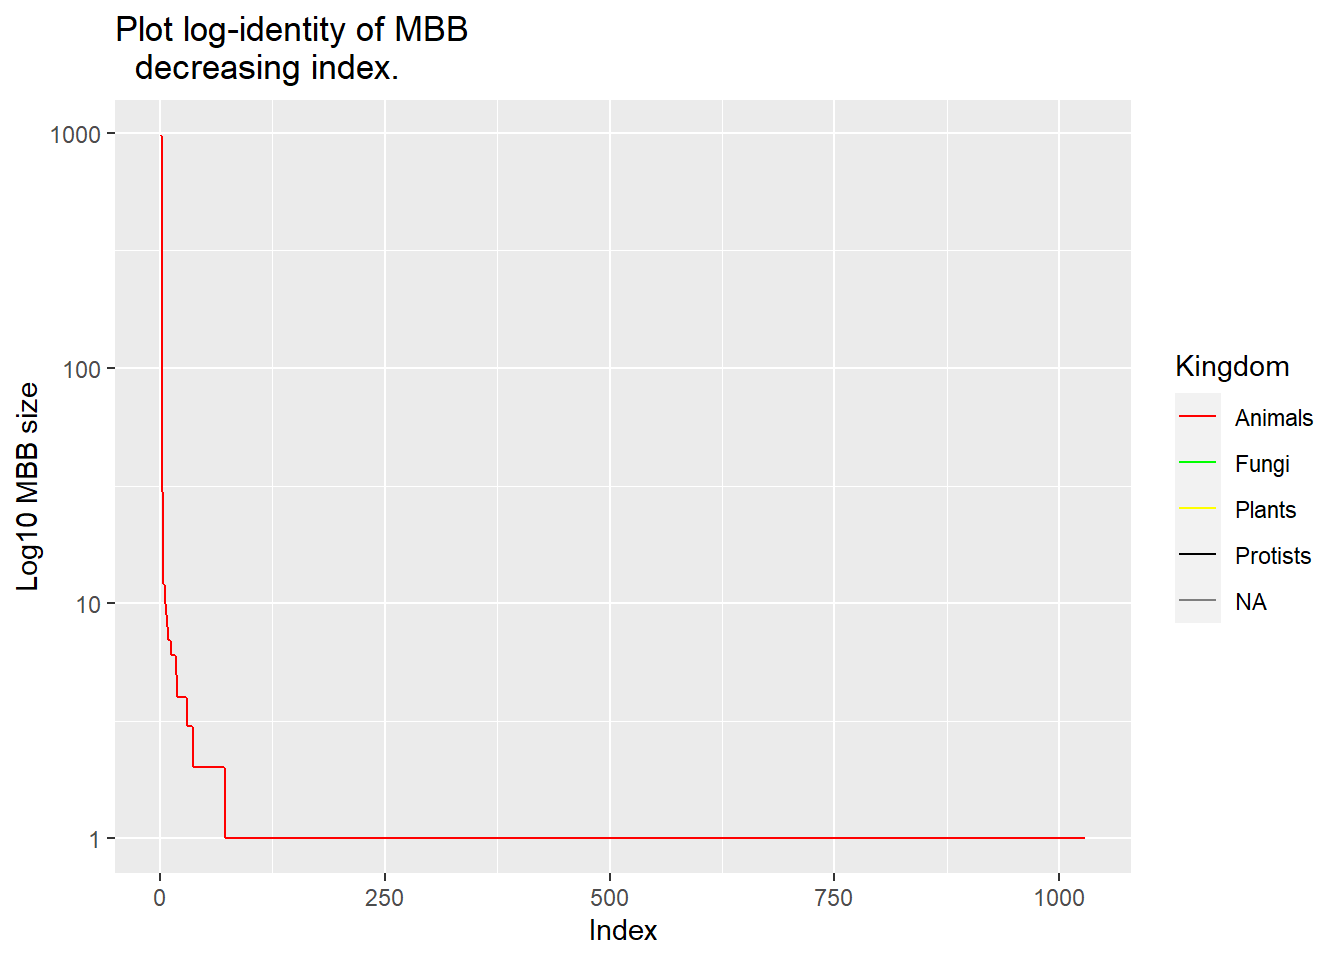
\includegraphics[width=1\textwidth,height=\textheight]{index_files/figure-pdf/unnamed-chunk-28-1.pdf}

}

\end{figure}

\begin{Shaded}
\begin{Highlighting}[]
\NormalTok{p1}
\end{Highlighting}
\end{Shaded}

\begin{figure}[H]

{\centering 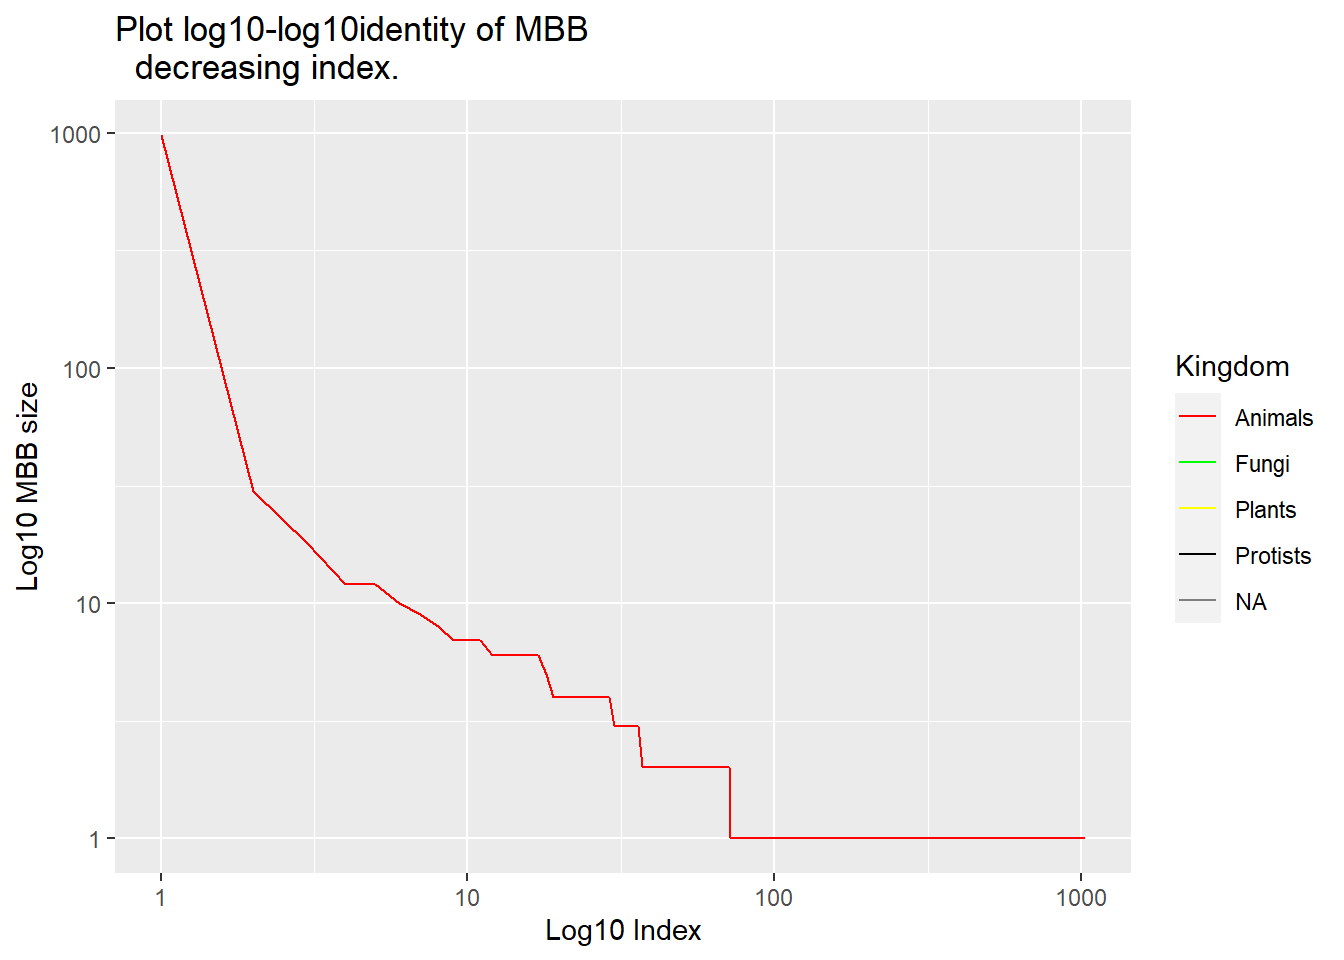
\includegraphics[width=1\textwidth,height=\textheight]{index_files/figure-pdf/unnamed-chunk-28-2.pdf}

}

\end{figure}

\begin{Shaded}
\begin{Highlighting}[]
\NormalTok{p2}
\end{Highlighting}
\end{Shaded}

\begin{figure}[H]

{\centering 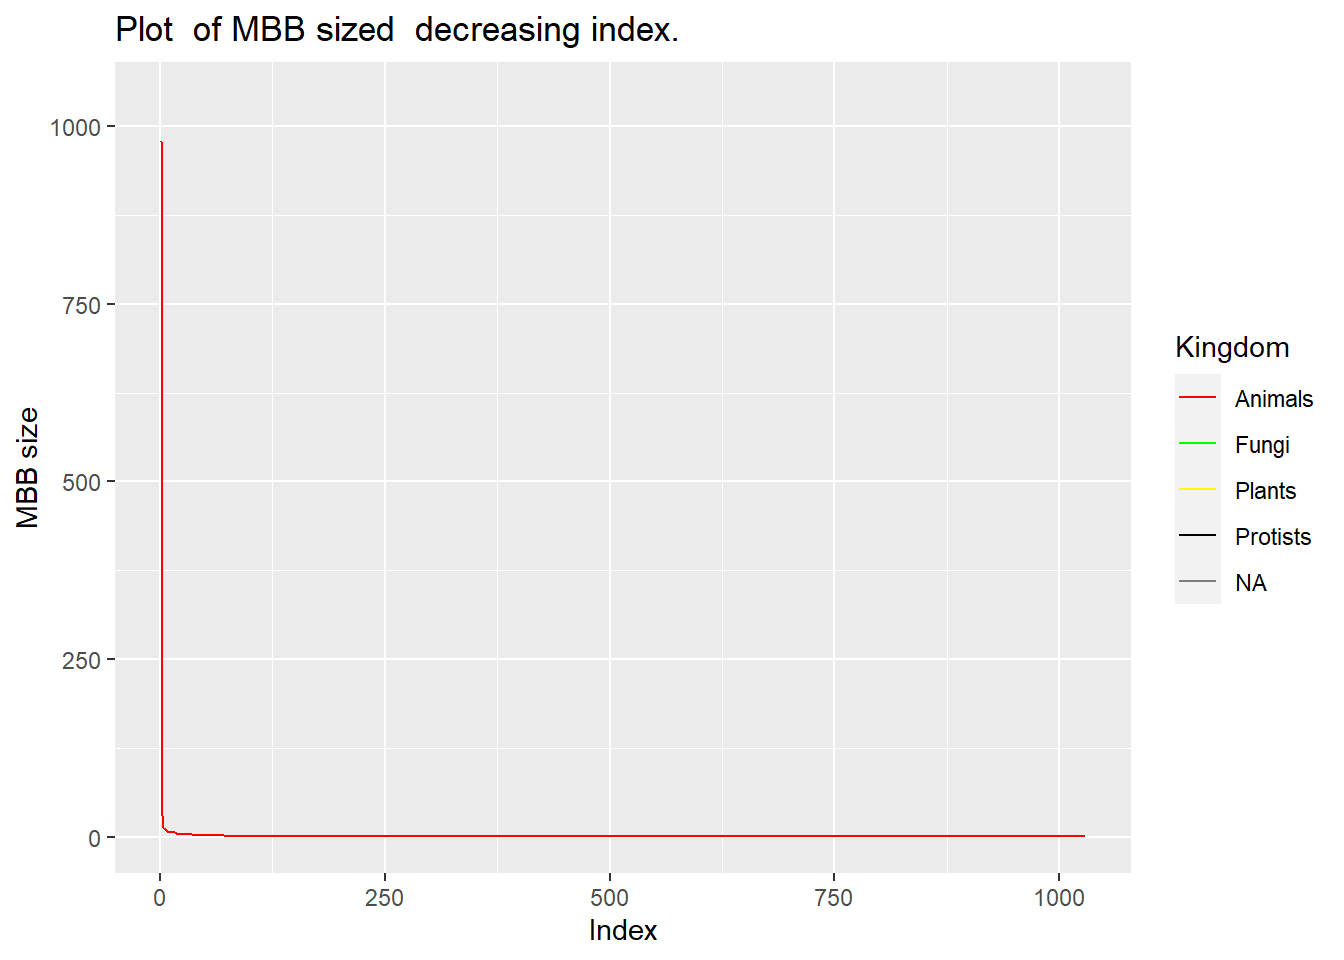
\includegraphics[width=1\textwidth,height=\textheight]{index_files/figure-pdf/unnamed-chunk-28-3.pdf}

}

\end{figure}

Additionally, we visualize the sizes of the MBBs of each m-DAG, using
colors to represent the different Kingdoms:

\begin{Shaded}
\begin{Highlighting}[]
\NormalTok{COLOR\_KINGDOM}\OtherTok{=}\FunctionTok{c}\NormalTok{(}\StringTok{"red"}\NormalTok{,}\StringTok{"yellow"}\NormalTok{,}\StringTok{"green"}\NormalTok{,}\StringTok{"yellow"}\NormalTok{,}\StringTok{"black"}\NormalTok{)}
\NormalTok{colors\_kingdom}\OtherTok{=}\NormalTok{aux2}\SpecialCharTok{\%\textgreater{}\%} \FunctionTok{select}\NormalTok{(Organism,Kingdom) }\SpecialCharTok{\%\textgreater{}\%} \FunctionTok{distinct}\NormalTok{()}
\FunctionTok{names}\NormalTok{(COLOR\_KINGDOM)}\OtherTok{=}\FunctionTok{sort}\NormalTok{(}\FunctionTok{unique}\NormalTok{(colors\_kingdom}\SpecialCharTok{$}\NormalTok{Kingdom))}

\NormalTok{p0}\OtherTok{\textless{}{-}}\FunctionTok{ggplot}\NormalTok{(}\AttributeTok{data=}\NormalTok{aux2) }\SpecialCharTok{+} 
  \FunctionTok{geom\_line}\NormalTok{(}\AttributeTok{mapping=}\FunctionTok{aes}\NormalTok{(}\AttributeTok{x=}\NormalTok{index,}
                        \AttributeTok{y=}\NormalTok{csize,}
                        \AttributeTok{group =}\NormalTok{ Organism,}
                        \AttributeTok{color=}\NormalTok{Kingdom),}
            \AttributeTok{na.rm=}\ConstantTok{TRUE}\NormalTok{) }\SpecialCharTok{+} 
  \FunctionTok{scale\_x\_continuous}\NormalTok{(}\AttributeTok{trans=}\StringTok{\textquotesingle{}log10\textquotesingle{}}\NormalTok{) }\SpecialCharTok{+} 
  \FunctionTok{scale\_y\_continuous}\NormalTok{(}\AttributeTok{trans=}\StringTok{\textquotesingle{}identity\textquotesingle{}}\NormalTok{) }\SpecialCharTok{+}
  \FunctionTok{scale\_color\_manual}\NormalTok{(}\AttributeTok{values =}\NormalTok{COLOR\_KINGDOM[colors\_kingdom}\SpecialCharTok{$}\NormalTok{Kingdom]) }\SpecialCharTok{+}
   \FunctionTok{ggtitle}\NormalTok{(}\StringTok{"Plot log{-}identity of size  weak components decreasing order"}\NormalTok{) }\SpecialCharTok{+}
  \FunctionTok{ylab}\NormalTok{(}\StringTok{"Log10 Weak componente size"}\NormalTok{) }\SpecialCharTok{+} \FunctionTok{xlab}\NormalTok{(}\StringTok{"Order"}\NormalTok{)}


\NormalTok{p1}\OtherTok{\textless{}{-}} \FunctionTok{ggplot}\NormalTok{(}\AttributeTok{data=}\NormalTok{aux2) }\SpecialCharTok{+} 
  \FunctionTok{geom\_line}\NormalTok{(}\AttributeTok{mapping=}\FunctionTok{aes}\NormalTok{(}\AttributeTok{x=}\NormalTok{index,}
                        \AttributeTok{y=}\NormalTok{csize,}\AttributeTok{group =}\NormalTok{ Organism,}
                        \AttributeTok{color=}\NormalTok{Kingdom),}
            \AttributeTok{na.rm=}\ConstantTok{TRUE}\NormalTok{) }\SpecialCharTok{+} 
  \FunctionTok{scale\_y\_continuous}\NormalTok{(}\AttributeTok{trans=}\StringTok{\textquotesingle{}log10\textquotesingle{}}\NormalTok{) }\SpecialCharTok{+} 
  \FunctionTok{scale\_x\_continuous}\NormalTok{(}\AttributeTok{trans=}\StringTok{\textquotesingle{}log10\textquotesingle{}}\NormalTok{) }\SpecialCharTok{+}
  \FunctionTok{scale\_color\_manual}\NormalTok{(}\AttributeTok{values =}\NormalTok{COLOR\_KINGDOM[colors\_kingdom}\SpecialCharTok{$}\NormalTok{Kingdom])}\SpecialCharTok{+}
   \FunctionTok{ggtitle}\NormalTok{(}\StringTok{"Plot log10{-}log10 of size  weak components decreasing order."}\NormalTok{) }\SpecialCharTok{+}
  \FunctionTok{ylab}\NormalTok{(}\StringTok{"Log10 weak component size"}\NormalTok{) }\SpecialCharTok{+} \FunctionTok{xlab}\NormalTok{(}\StringTok{"Log10 order"}\NormalTok{)}

\NormalTok{p2}\OtherTok{\textless{}{-}} \FunctionTok{ggplot}\NormalTok{(}\AttributeTok{data=}\NormalTok{aux2) }\SpecialCharTok{+} 
  \FunctionTok{geom\_line}\NormalTok{(}\AttributeTok{mapping=}\FunctionTok{aes}\NormalTok{(}\AttributeTok{x=}\NormalTok{index,}
                        \AttributeTok{y=}\NormalTok{csize,}\AttributeTok{group =}\NormalTok{ Organism,}
                        \AttributeTok{color=}\NormalTok{Kingdom),}
            \AttributeTok{na.rm=}\ConstantTok{TRUE}\NormalTok{) }\SpecialCharTok{+} 
   \FunctionTok{scale\_x\_continuous}\NormalTok{(}\AttributeTok{trans=}\StringTok{"identity"}\NormalTok{) }\SpecialCharTok{+} 
  \FunctionTok{scale\_y\_continuous}\NormalTok{(}\AttributeTok{trans=}\StringTok{"identity"}\NormalTok{) }\SpecialCharTok{+}
  \FunctionTok{ylim}\NormalTok{(}\DecValTok{0}\NormalTok{,}\DecValTok{1039}\NormalTok{)}\SpecialCharTok{+}
   \FunctionTok{ggtitle}\NormalTok{(}\StringTok{"Plot  of size  weak components decreasing order."}\NormalTok{)}\SpecialCharTok{+}
  \FunctionTok{ylab}\NormalTok{(}\StringTok{"Weak components size"}\NormalTok{) }\SpecialCharTok{+} \FunctionTok{xlab}\NormalTok{(}\StringTok{"Order"}\NormalTok{)}\SpecialCharTok{+}
  \FunctionTok{scale\_color\_manual}\NormalTok{(}\AttributeTok{values =}\NormalTok{COLOR\_KINGDOM[colors\_kingdom}\SpecialCharTok{$}\NormalTok{Kingdom])}


\NormalTok{p0}
\end{Highlighting}
\end{Shaded}

\begin{figure}[H]

{\centering 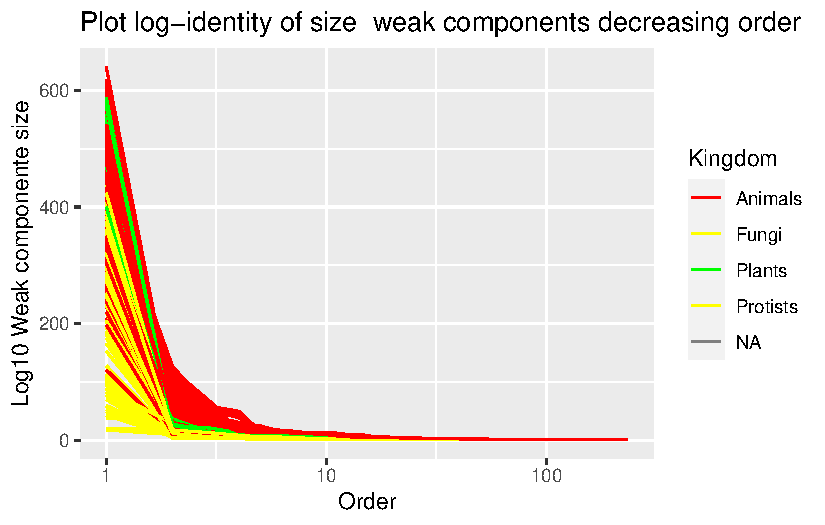
\includegraphics[width=1\textwidth,height=\textheight]{index_files/figure-pdf/unnamed-chunk-29-1.pdf}

}

\end{figure}

\begin{Shaded}
\begin{Highlighting}[]
\NormalTok{p1}
\end{Highlighting}
\end{Shaded}

\begin{figure}[H]

{\centering 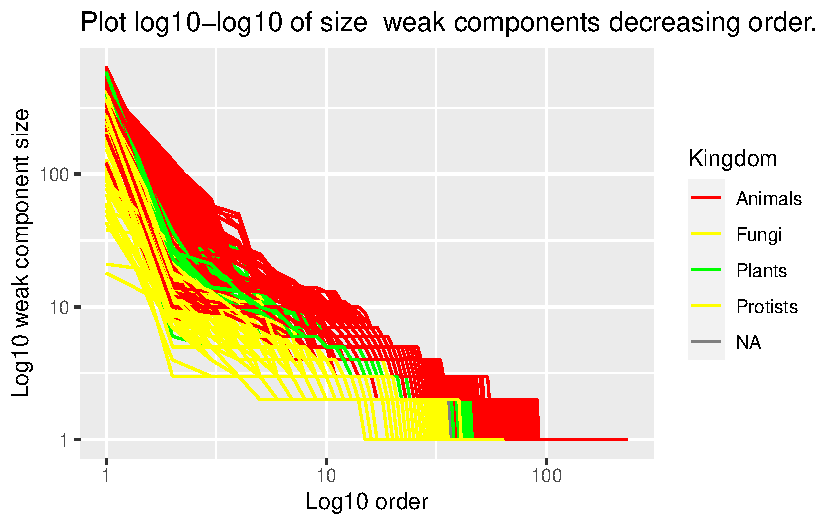
\includegraphics[width=1\textwidth,height=\textheight]{index_files/figure-pdf/unnamed-chunk-29-2.pdf}

}

\end{figure}

\begin{Shaded}
\begin{Highlighting}[]
\NormalTok{p2}
\end{Highlighting}
\end{Shaded}

\begin{figure}[H]

{\centering 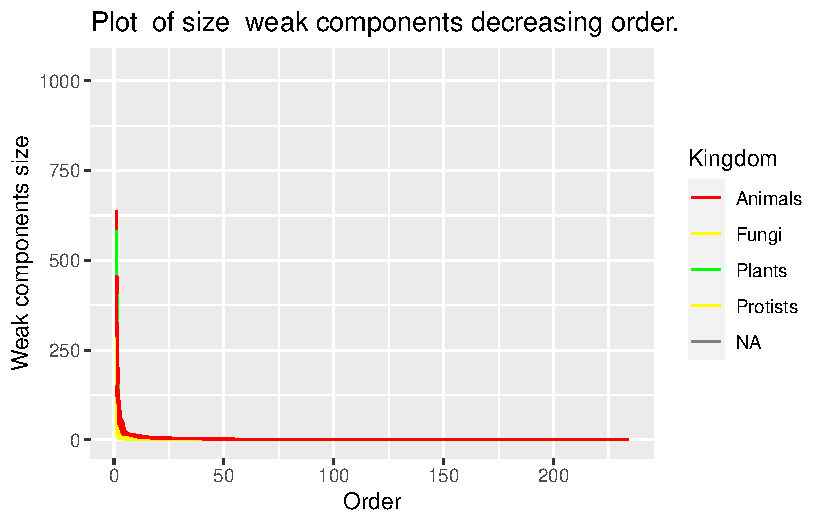
\includegraphics[width=1\textwidth,height=\textheight]{index_files/figure-pdf/unnamed-chunk-29-3.pdf}

}

\end{figure}

\begin{Shaded}
\begin{Highlighting}[]
\NormalTok{data2}\OtherTok{=}\NormalTok{big\_MBB\_list2 }\SpecialCharTok{\%\textgreater{}\%} \FunctionTok{filter}\NormalTok{(index }\SpecialCharTok{\%in\%} \DecValTok{2}\SpecialCharTok{:}\DecValTok{20}\NormalTok{)}
\NormalTok{p3}\OtherTok{\textless{}{-}} \FunctionTok{ggplot}\NormalTok{(}\AttributeTok{data=}\NormalTok{data2) }\SpecialCharTok{+} 
  \FunctionTok{geom\_line}\NormalTok{(}\AttributeTok{mapping=}\FunctionTok{aes}\NormalTok{(}\AttributeTok{x=}\NormalTok{index,}
                        \AttributeTok{y=}\NormalTok{MBBsize,}
                        \AttributeTok{group =}\NormalTok{ Organism,}
                        \AttributeTok{color=}\NormalTok{Kingdom),}
            \AttributeTok{na.rm=}\ConstantTok{TRUE}\NormalTok{)}\SpecialCharTok{+}
  \FunctionTok{scale\_x\_continuous}\NormalTok{(}\AttributeTok{trans=}\StringTok{"identity"}\NormalTok{) }\SpecialCharTok{+} 
  \FunctionTok{scale\_y\_continuous}\NormalTok{(}\AttributeTok{trans=}\StringTok{"identity"}\NormalTok{) }\SpecialCharTok{+}
  \FunctionTok{ylim}\NormalTok{(}\DecValTok{0}\NormalTok{,}\DecValTok{25}\NormalTok{)}\SpecialCharTok{+}
  \FunctionTok{ggtitle}\NormalTok{(}\StringTok{"Plot  of size  weak components  decreasing order 2 to 20."}\NormalTok{)}\SpecialCharTok{+}
  \FunctionTok{ylab}\NormalTok{(}\StringTok{"Weak components size"}\NormalTok{) }\SpecialCharTok{+} \FunctionTok{xlab}\NormalTok{(}\StringTok{"Order"}\NormalTok{)}\SpecialCharTok{+}
  \FunctionTok{scale\_color\_manual}\NormalTok{(}\AttributeTok{values =}\NormalTok{COLOR\_KINGDOM[colors\_kingdom}\SpecialCharTok{$}\NormalTok{Kingdom])}

\NormalTok{p3}
\end{Highlighting}
\end{Shaded}

\begin{figure}[H]

{\centering 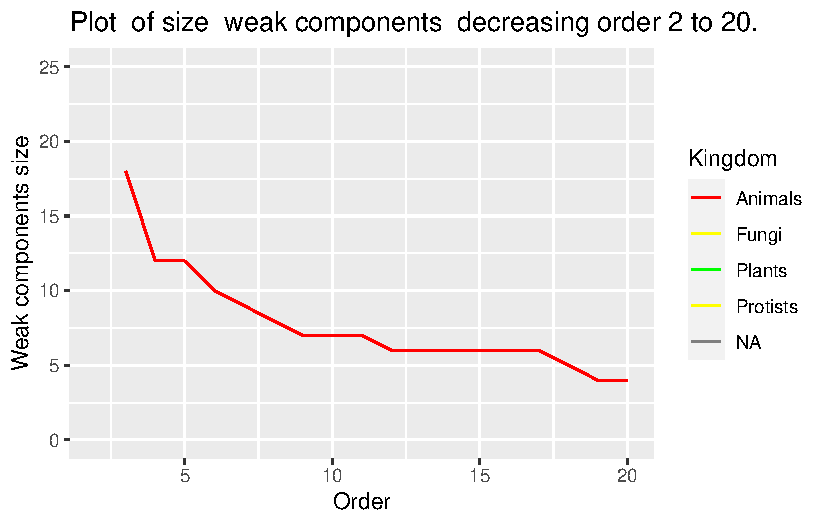
\includegraphics[width=1\textwidth,height=\textheight]{index_files/figure-pdf/unnamed-chunk-30-1.pdf}

}

\end{figure}

\bookmarksetup{startatroot}

\hypertarget{m-dags-similarities-and-metadata}{%
\chapter{m-DAGs similarities and
Metadata}\label{m-dags-similarities-and-metadata}}

First, we will load the metadata and adjust them to match the structure
of the similarities. This will facilitate the creation of graphs and
statistics.

Keep in mind the path of the experiment:

\begin{Shaded}
\begin{Highlighting}[]
\NormalTok{path\_exp}
\end{Highlighting}
\end{Shaded}

\begin{verbatim}
[1] "data/result_0a845f74-826e-3b46-aed9-e7ecf74db262/"
\end{verbatim}

\hypertarget{msa-munkres-similarities}{%
\section{MSA \& Munkres similarities}\label{msa-munkres-similarities}}

In this section, we will present the similarities between m-DAGs
considering the two similarity meausures described in the paper. Namely,
the MSA and Munkres similarities.

The experimental data set consists of 1132 Eukaryotes from the animal,
plant, fungus, and protists kingdoms.

\begin{tabular}{l|r}
\hline
Kingdom & Abs. Freq.\\
\hline
Animals & 535\\
\hline
Fungi & 154\\
\hline
Plants & 139\\
\hline
Protists & 56\\
\hline
\end{tabular}

The similarity values are provided in the following files:

\begin{Shaded}
\begin{Highlighting}[]
\NormalTok{list\_Sim}\OtherTok{=}\FunctionTok{dir}\NormalTok{(path\_exp,}\AttributeTok{pattern=}\StringTok{"\^{}Similarities"}\NormalTok{)}
\NormalTok{list\_Sim}
\end{Highlighting}
\end{Shaded}

\begin{verbatim}
[1] "Similarities_MBB_MSAMethod.csv"      "Similarities_MBB_MunkresMethod.csv" 
[3] "Similarities_mDAG_MSAMethod.csv"     "Similarities_mDAG_MunkresMethod.csv"
\end{verbatim}

Load the m-DAGs similarities

\begin{Shaded}
\begin{Highlighting}[]
\NormalTok{Sim\_MSA\_mDAG}\OtherTok{=}\FunctionTok{read\_csv}\NormalTok{(}\FunctionTok{paste0}\NormalTok{(path\_exp,}
                             \StringTok{"Similarities\_mDAG\_MSAMethod.csv"}\NormalTok{))}
\NormalTok{Sim\_MSA\_mDAG}\OtherTok{=}\FunctionTok{as.matrix}\NormalTok{(Sim\_MSA\_mDAG[,}\SpecialCharTok{{-}}\DecValTok{1}\NormalTok{])}
\FunctionTok{rownames}\NormalTok{(Sim\_MSA\_mDAG)}\OtherTok{=}\FunctionTok{colnames}\NormalTok{(Sim\_MSA\_mDAG)}
\NormalTok{Sim\_MSA\_mDAG}\OtherTok{=}\NormalTok{Sim\_MSA\_mDAG[meta\_taxo}\SpecialCharTok{$}\NormalTok{mDAG\_Id[}\DecValTok{1}\SpecialCharTok{:}\DecValTok{884}\NormalTok{],}
\NormalTok{                          meta\_taxo}\SpecialCharTok{$}\NormalTok{mDAG\_Id[}\DecValTok{1}\SpecialCharTok{:}\DecValTok{884}\NormalTok{]]}
\end{Highlighting}
\end{Shaded}

\begin{Shaded}
\begin{Highlighting}[]
\NormalTok{Sim\_Mun\_mDAG}\OtherTok{=}\FunctionTok{read\_csv}\NormalTok{(}\FunctionTok{paste0}\NormalTok{(path\_exp,}\StringTok{"Similarities\_mDAG\_MunkresMethod.csv"}\NormalTok{))}
\NormalTok{Sim\_Mun\_mDAG}\OtherTok{=}\FunctionTok{as.matrix}\NormalTok{(Sim\_Mun\_mDAG[,}\SpecialCharTok{{-}}\DecValTok{1}\NormalTok{])}
\FunctionTok{rownames}\NormalTok{(Sim\_Mun\_mDAG)}\OtherTok{=}\FunctionTok{colnames}\NormalTok{(Sim\_Mun\_mDAG)}
\NormalTok{Sim\_Mun\_mDAG}\OtherTok{=}\NormalTok{Sim\_Mun\_mDAG[meta\_taxo}\SpecialCharTok{$}\NormalTok{mDAG\_Id[}\DecValTok{1}\SpecialCharTok{:}\DecValTok{884}\NormalTok{],meta\_taxo}\SpecialCharTok{$}\NormalTok{mDAG\_Id[}\DecValTok{1}\SpecialCharTok{:}\DecValTok{884}\NormalTok{]]}
\end{Highlighting}
\end{Shaded}

\hypertarget{heatmaps}{%
\section{Heatmaps}\label{heatmaps}}

Here, we provide examples of heatmaps to visualize the similarities
betweem m-DAGs. We again consider colors to represent the different
Kingdoms.

\begin{Shaded}
\begin{Highlighting}[]
\NormalTok{dff}\OtherTok{\textless{}{-}}\NormalTok{meta\_taxo[}\DecValTok{1}\SpecialCharTok{:}\DecValTok{884}\NormalTok{,] }\SpecialCharTok{\%\textgreater{}\%} \FunctionTok{select}\NormalTok{(Kingdom)  }\SpecialCharTok{\%\textgreater{}\%} \FunctionTok{as.data.frame}\NormalTok{()}
\NormalTok{colorsK }\OtherTok{\textless{}{-}} \FunctionTok{list}\NormalTok{(}\AttributeTok{Kingdom=} \FunctionTok{c}\NormalTok{(}\StringTok{"Animals"}\OtherTok{=}\StringTok{"red"}\NormalTok{,}
                           \StringTok{"Plants"}\OtherTok{=}\StringTok{"green"}\NormalTok{,}
                           \StringTok{"Fungi"}\OtherTok{=}\StringTok{"yellow"}\NormalTok{,}
                           \StringTok{"Protists"}\OtherTok{=}\StringTok{"black"}\NormalTok{))}
\NormalTok{annotationK }\OtherTok{\textless{}{-}} \FunctionTok{HeatmapAnnotation}\NormalTok{(}\AttributeTok{df=}\NormalTok{dff, }\AttributeTok{col =}\NormalTok{ colorsK,}\AttributeTok{show\_legend =} \ConstantTok{TRUE}\NormalTok{)}

\NormalTok{MSA\_heat\_1 }\OtherTok{\textless{}{-}} \FunctionTok{Heatmap}\NormalTok{(}\AttributeTok{matrix =}\NormalTok{ Sim\_MSA\_mDAG, }
                      \AttributeTok{column\_title=}
                        \StringTok{"m{-}DAGs MSA{-}similarity Eukaryotes by Kingdoms"}\NormalTok{,}
                      \AttributeTok{heatmap\_legend\_param=}\FunctionTok{list}\NormalTok{(}
                        \AttributeTok{title=}\StringTok{"Similarity"}\NormalTok{,}
                        \AttributeTok{at =} \FunctionTok{seq}\NormalTok{(}\DecValTok{0}\NormalTok{,}\DecValTok{1}\NormalTok{,}\AttributeTok{by=}\FloatTok{0.1}\NormalTok{)),}
                      \AttributeTok{col=}\FunctionTok{rev}\NormalTok{(}\FunctionTok{viridis}\NormalTok{(}\DecValTok{256}\NormalTok{)),}
                      \AttributeTok{cluster\_rows =} \ConstantTok{FALSE}\NormalTok{,}
                      \AttributeTok{cluster\_columns =} \ConstantTok{FALSE}\NormalTok{,}
                      \AttributeTok{top\_annotation =}\NormalTok{ annotationK,}
                      \AttributeTok{show\_column\_names =} \ConstantTok{FALSE}\NormalTok{, }
                      \AttributeTok{show\_row\_names =} \ConstantTok{FALSE}\NormalTok{,}
                      \AttributeTok{left\_annotation =}
                        \FunctionTok{rowAnnotation}\NormalTok{(}\AttributeTok{df =}\NormalTok{ dff,}
                                      \AttributeTok{col =}\NormalTok{ colorsK,}
                                    \AttributeTok{show\_annotation\_name=}\ConstantTok{FALSE}\NormalTok{,}
                                    \AttributeTok{show\_legend=}\ConstantTok{FALSE}
\NormalTok{                                      ))}







\NormalTok{Mun\_heat\_1}\OtherTok{\textless{}{-}} \FunctionTok{Heatmap}\NormalTok{(}\AttributeTok{matrix =}\NormalTok{ Sim\_Mun\_mDAG, }
             \AttributeTok{column\_title=}\StringTok{"mDAGs Munkres{-}similarity  Eukaryotes by Kingdoms"}\NormalTok{,}
            \AttributeTok{name =} \StringTok{"Munkres Similarity"}\NormalTok{,}
            \AttributeTok{heatmap\_legend\_param=}\FunctionTok{list}\NormalTok{(}
                        \AttributeTok{title=}\StringTok{"Similarity"}\NormalTok{,}
                        \AttributeTok{at =} \FunctionTok{seq}\NormalTok{(}\DecValTok{0}\NormalTok{,}\DecValTok{1}\NormalTok{,}\AttributeTok{by=}\FloatTok{0.1}\NormalTok{)),}
                      \AttributeTok{col=}\FunctionTok{rev}\NormalTok{(}\FunctionTok{viridis}\NormalTok{(}\DecValTok{256}\NormalTok{)),}
                      \AttributeTok{cluster\_rows =} \ConstantTok{FALSE}\NormalTok{,}
                      \AttributeTok{cluster\_columns =} \ConstantTok{FALSE}\NormalTok{,}
                      \AttributeTok{top\_annotation =}\NormalTok{ annotationK,}
                      \AttributeTok{show\_column\_names =} \ConstantTok{FALSE}\NormalTok{, }
                      \AttributeTok{show\_row\_names =} \ConstantTok{FALSE}\NormalTok{,}
                      \AttributeTok{left\_annotation =}
                        \FunctionTok{rowAnnotation}\NormalTok{(}\AttributeTok{df =}\NormalTok{ dff,}
                                      \AttributeTok{col =}\NormalTok{ colorsK,}
                                    \AttributeTok{show\_annotation\_name=}\ConstantTok{FALSE}\NormalTok{,}
                                    \AttributeTok{show\_legend=}\ConstantTok{FALSE}
\NormalTok{                                      ))}
\end{Highlighting}
\end{Shaded}

\begin{Shaded}
\begin{Highlighting}[]
\NormalTok{meta\_animals}\OtherTok{=}\NormalTok{ meta\_taxo[}\DecValTok{1}\SpecialCharTok{:}\DecValTok{884}\NormalTok{,] }\SpecialCharTok{\%\textgreater{}\%} \FunctionTok{filter}\NormalTok{(Kingdom}\SpecialCharTok{==}\StringTok{"Animals"}\NormalTok{)}

\NormalTok{dff}\OtherTok{\textless{}{-}}\NormalTok{meta\_taxo }\SpecialCharTok{\%\textgreater{}\%}
  \FunctionTok{filter}\NormalTok{(Kingdom}\SpecialCharTok{==}\StringTok{"Animals"}\NormalTok{) }\SpecialCharTok{\%\textgreater{}\%} 
  \FunctionTok{select}\NormalTok{(Phylum,Freq\_Phylum) }\SpecialCharTok{\%\textgreater{}\%}   
  \FunctionTok{as.data.frame}\NormalTok{() }\SpecialCharTok{\%\textgreater{}\%} \FunctionTok{select}\NormalTok{(Phylum)}

\NormalTok{namesP}\OtherTok{=}\NormalTok{dff }\SpecialCharTok{\%\textgreater{}\%} \FunctionTok{distinct}\NormalTok{( Phylum, }\AttributeTok{.keep\_all =} \ConstantTok{TRUE}\NormalTok{) }
\NormalTok{namesP}\OtherTok{=}\NormalTok{namesP}\SpecialCharTok{$}\NormalTok{Phylum}
\NormalTok{dff}\SpecialCharTok{$}\NormalTok{Phylum}\OtherTok{=}\FunctionTok{ordered}\NormalTok{(dff}\SpecialCharTok{$}\NormalTok{Phylum,}\AttributeTok{labels=}\NormalTok{namesP)}
\NormalTok{col}\OtherTok{=}\FunctionTok{rainbow}\NormalTok{(}\FunctionTok{length}\NormalTok{(namesP))}
\NormalTok{colorsP}\OtherTok{=}\FunctionTok{list}\NormalTok{(}\AttributeTok{Phylum=}\NormalTok{col)}
\FunctionTok{names}\NormalTok{(colorsP}\SpecialCharTok{$}\NormalTok{Phylum)}\OtherTok{=}\NormalTok{namesP}
\NormalTok{annotation\_H2 }\OtherTok{\textless{}{-}} \FunctionTok{HeatmapAnnotation}\NormalTok{(}\AttributeTok{df=}\NormalTok{dff, }\AttributeTok{col =}\NormalTok{ colorsP)}
\NormalTok{MSA\_heat\_2 }\OtherTok{\textless{}{-}} \FunctionTok{Heatmap}\NormalTok{(}\AttributeTok{matrix =}
\NormalTok{                        Sim\_MSA\_mDAG[}\DecValTok{1}\SpecialCharTok{:}\FunctionTok{nrow}\NormalTok{(dff),}\DecValTok{1}\SpecialCharTok{:}\FunctionTok{nrow}\NormalTok{(dff)],}
                      \AttributeTok{column\_title=}\StringTok{"mDAGs MSA{-}similarity  Animals by Phyla"}\NormalTok{,}
                      \AttributeTok{col=}\FunctionTok{rev}\NormalTok{(}\FunctionTok{viridis}\NormalTok{(}\DecValTok{256}\NormalTok{)),}
                      \AttributeTok{cluster\_rows =} \ConstantTok{FALSE}\NormalTok{,}
                      \AttributeTok{show\_heatmap\_legend=}\ConstantTok{FALSE}\NormalTok{, }
                      \AttributeTok{cluster\_columns =} \ConstantTok{FALSE}\NormalTok{,}
                      \AttributeTok{top\_annotation =}\NormalTok{ annotation\_H2,}
                      \AttributeTok{show\_column\_names =} \ConstantTok{FALSE}\NormalTok{, }
                      \AttributeTok{show\_row\_names =} \ConstantTok{FALSE}\NormalTok{,}
                      \AttributeTok{left\_annotation =} 
                        \FunctionTok{rowAnnotation}\NormalTok{(}\AttributeTok{df =}\NormalTok{ dff,}
                                      \AttributeTok{col =}\NormalTok{ colorsP,}
                                      \AttributeTok{show\_annotation\_name=}\ConstantTok{FALSE}\NormalTok{,}
                                      \AttributeTok{show\_legend =}\ConstantTok{FALSE}
\NormalTok{                                      ))}



\NormalTok{Mun\_heat\_2 }\OtherTok{\textless{}{-}} \FunctionTok{Heatmap}\NormalTok{(}\AttributeTok{matrix =}\NormalTok{ Sim\_Mun\_mDAG[}\DecValTok{1}\SpecialCharTok{:}\FunctionTok{nrow}\NormalTok{(dff),}\DecValTok{1}\SpecialCharTok{:}\FunctionTok{nrow}\NormalTok{(dff)], }
              \AttributeTok{column\_title=}\StringTok{"mDAGs Munkres{-}similarity  Animals by Phyla"}\NormalTok{,}
        \AttributeTok{col=}\FunctionTok{rev}\NormalTok{(}\FunctionTok{viridis}\NormalTok{(}\DecValTok{256}\NormalTok{)),}
    \AttributeTok{show\_heatmap\_legend=}\ConstantTok{FALSE}\NormalTok{, }
        \AttributeTok{cluster\_rows =} \ConstantTok{FALSE}\NormalTok{,}
        \AttributeTok{cluster\_columns =} \ConstantTok{FALSE}\NormalTok{,}
        \AttributeTok{top\_annotation =}\NormalTok{ annotation\_H2,}
        \AttributeTok{show\_column\_names =} \ConstantTok{FALSE}\NormalTok{, }
        \AttributeTok{show\_row\_names =} \ConstantTok{FALSE}\NormalTok{,}
        \AttributeTok{left\_annotation =} \FunctionTok{rowAnnotation}\NormalTok{(}\AttributeTok{df =}\NormalTok{ dff,}
                                        \AttributeTok{col =}\NormalTok{ colorsP,}
                                    \AttributeTok{show\_annotation\_name=}\ConstantTok{FALSE}\NormalTok{,}
                                        \AttributeTok{show\_legend =}\ConstantTok{FALSE}
\NormalTok{                                        ))}
\end{Highlighting}
\end{Shaded}

\begin{Shaded}
\begin{Highlighting}[]
\NormalTok{MSA\_heat\_1}
\end{Highlighting}
\end{Shaded}

\begin{figure}[H]

{\centering 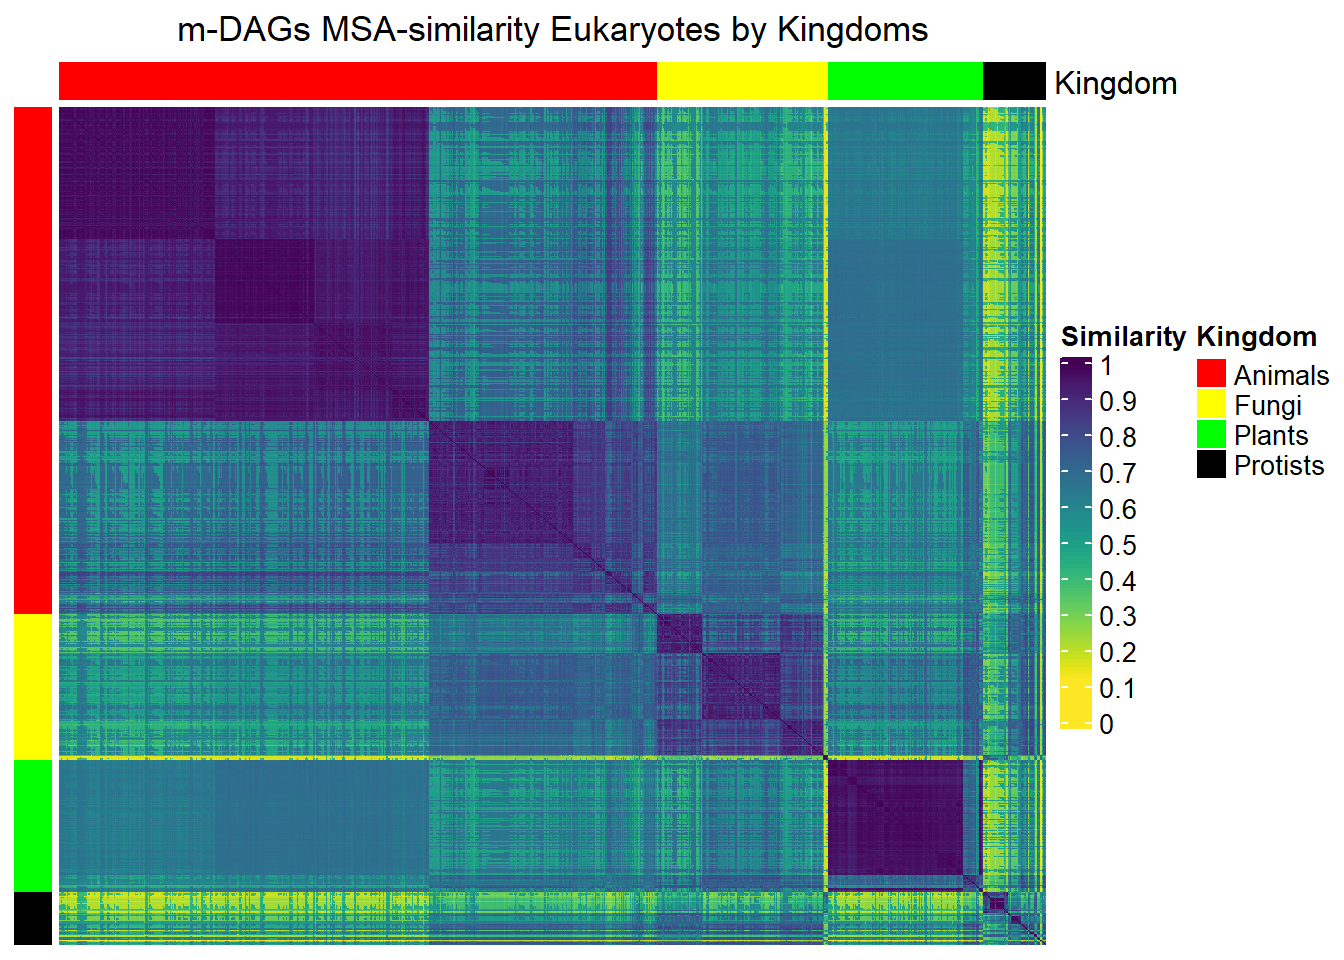
\includegraphics[width=1\textwidth,height=\textheight]{index_files/figure-pdf/heatmaps-1.pdf}

}

\end{figure}

\begin{Shaded}
\begin{Highlighting}[]
\NormalTok{MSA\_heat\_2}
\end{Highlighting}
\end{Shaded}

\begin{figure}[H]

{\centering 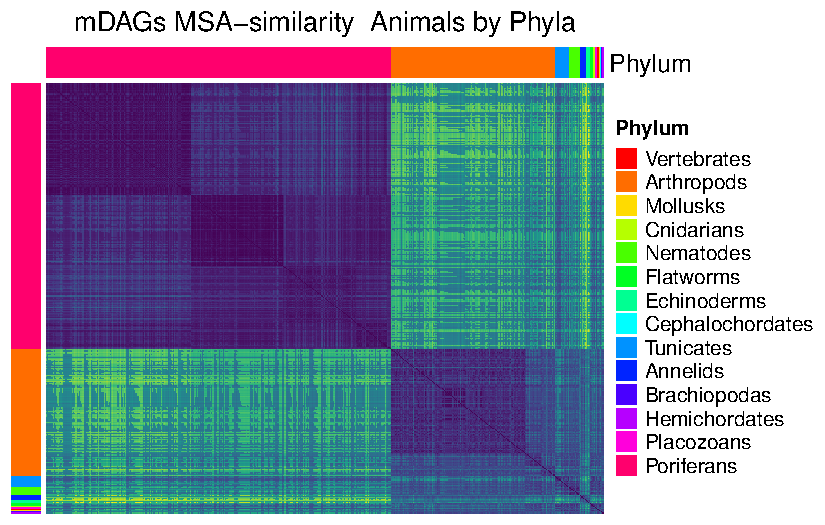
\includegraphics[width=1\textwidth,height=\textheight]{index_files/figure-pdf/heatmaps-2.pdf}

}

\end{figure}

\begin{Shaded}
\begin{Highlighting}[]
\NormalTok{Mun\_heat\_1}
\end{Highlighting}
\end{Shaded}

\begin{figure}[H]

{\centering 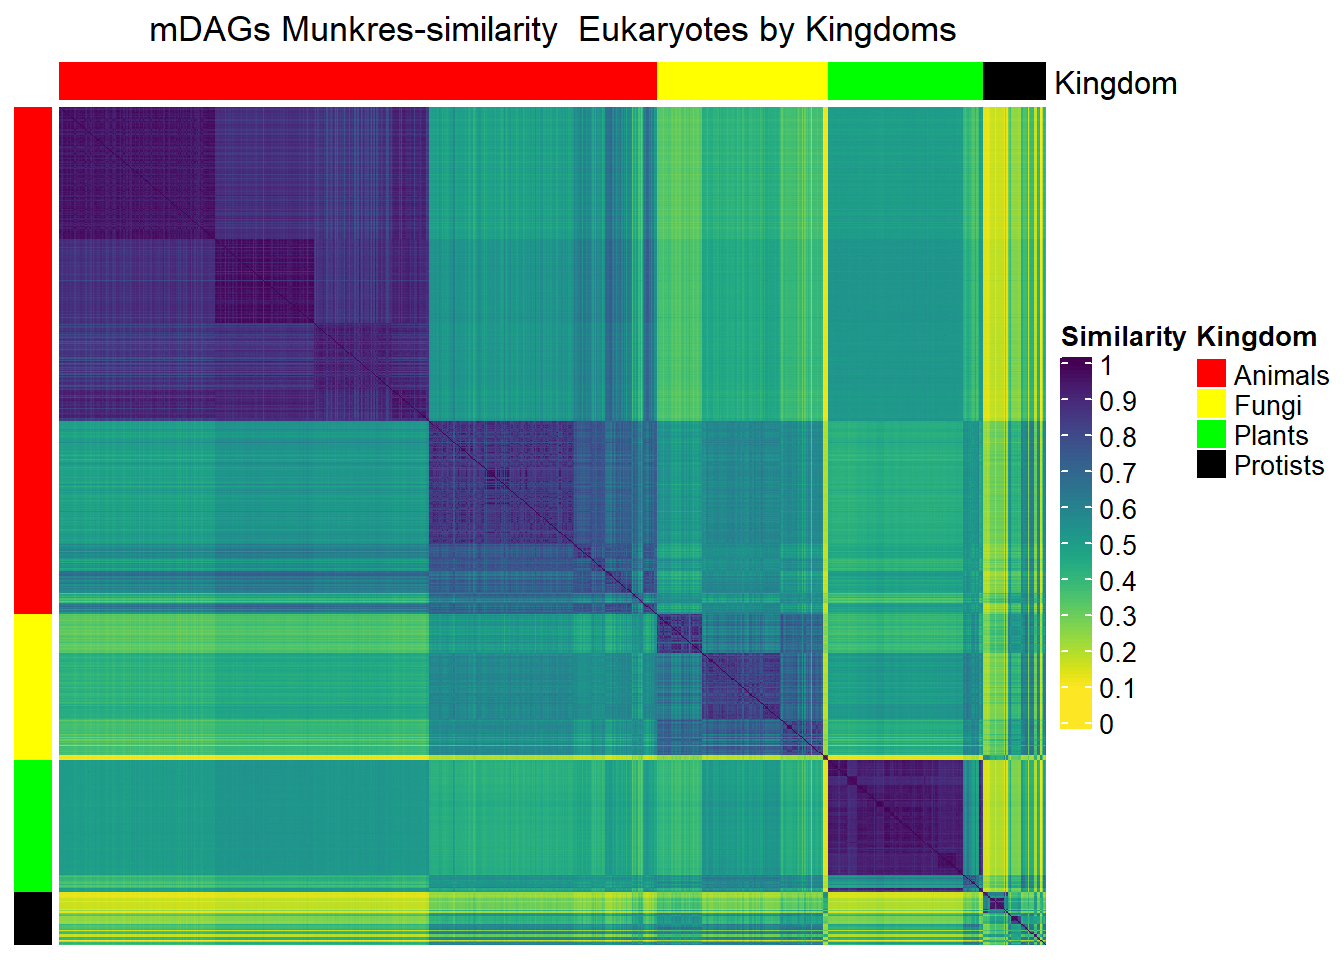
\includegraphics[width=1\textwidth,height=\textheight]{index_files/figure-pdf/heatmaps-3.pdf}

}

\end{figure}

\begin{Shaded}
\begin{Highlighting}[]
\NormalTok{Mun\_heat\_2}
\end{Highlighting}
\end{Shaded}

\begin{figure}[H]

{\centering 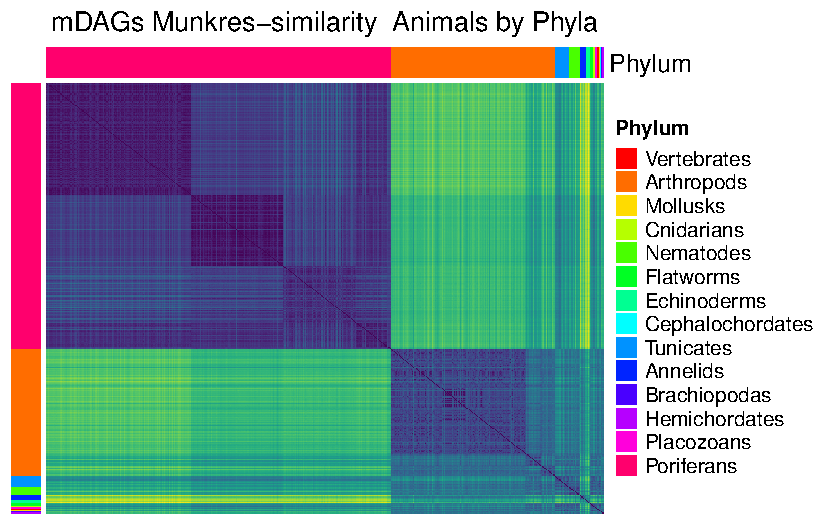
\includegraphics[width=1\textwidth,height=\textheight]{index_files/figure-pdf/heatmaps-4.pdf}

}

\end{figure}

\hypertarget{mds-multidimensional-scaling-msa-munkres-similarity}{%
\section{MDS (Multidimensional Scaling) MSA \& Munkres
similarity}\label{mds-multidimensional-scaling-msa-munkres-similarity}}

Multi-dimensional Scaling (MDS) is a classic multivariate data analysis
technique that allows for obtaining a low-dimensional representation of
the observed similarities.

The following is the MDS for the MSA similarity:

\begin{Shaded}
\begin{Highlighting}[]
\DocumentationTok{\#\# Metric multidimensional scaling (mMDS)}
\NormalTok{mds7 }\OtherTok{\textless{}{-}} \FunctionTok{cmdscale}\NormalTok{(}\FunctionTok{sqrt}\NormalTok{(}\DecValTok{1}\SpecialCharTok{{-}}\NormalTok{Sim\_MSA\_mDAG}\SpecialCharTok{\^{}}\DecValTok{2}\NormalTok{),}\AttributeTok{k=}\DecValTok{7}\NormalTok{,}\AttributeTok{eig=}\ConstantTok{TRUE}\NormalTok{)}
\CommentTok{\#pairs(mds7$points[,1:4])}
\NormalTok{mds7}\SpecialCharTok{$}\NormalTok{GOF}
\end{Highlighting}
\end{Shaded}

\begin{verbatim}
[1] 0.4449519 0.5570199
\end{verbatim}

\begin{Shaded}
\begin{Highlighting}[]
\NormalTok{mds }\OtherTok{\textless{}{-}}\NormalTok{ mds7}\SpecialCharTok{$}\NormalTok{points }\SpecialCharTok{\%\textgreater{}\%}  \FunctionTok{as\_tibble}\NormalTok{()}
\FunctionTok{colnames}\NormalTok{(mds) }\OtherTok{\textless{}{-}}\FunctionTok{paste0}\NormalTok{(}\StringTok{"Dim."}\NormalTok{,}\DecValTok{1}\SpecialCharTok{:}\FunctionTok{dim}\NormalTok{(mds7}\SpecialCharTok{$}\NormalTok{points)[}\DecValTok{2}\NormalTok{])}


\NormalTok{cooordinates}\OtherTok{=}\FunctionTok{as\_tibble}\NormalTok{(mds7}\SpecialCharTok{$}\NormalTok{points)}
\FunctionTok{colnames}\NormalTok{(cooordinates)}\OtherTok{=}\FunctionTok{paste}\NormalTok{(}\StringTok{"Component"}\NormalTok{,}\DecValTok{1}\SpecialCharTok{:}\DecValTok{7}\NormalTok{)}
\FunctionTok{ggpairs}\NormalTok{(cooordinates,}\AttributeTok{columns=}\DecValTok{1}\SpecialCharTok{:}\DecValTok{4}\NormalTok{,}
        \FunctionTok{aes}\NormalTok{(}\AttributeTok{color=}\NormalTok{meta\_taxo}\SpecialCharTok{$}\NormalTok{Kingdom[}\DecValTok{1}\SpecialCharTok{:}\DecValTok{884}\NormalTok{],}\AttributeTok{alpha=}\FloatTok{0.5}\NormalTok{,}
            \AttributeTok{title=}\StringTok{"MDS 4 dimensions projection"}\NormalTok{,}
            \AttributeTok{legend=}\DecValTok{1}\NormalTok{),}\AttributeTok{upper=}\FunctionTok{list}\NormalTok{(}\AttributeTok{continuous=}\StringTok{"points"}\NormalTok{)) }\SpecialCharTok{+}
  \FunctionTok{scale\_fill\_manual}\NormalTok{(}\AttributeTok{values =}\NormalTok{ colorsK}\SpecialCharTok{$}\NormalTok{Kingdom) }\SpecialCharTok{+} 
  \FunctionTok{theme}\NormalTok{(}\AttributeTok{legend.position =} \StringTok{"left"}\NormalTok{)}
\end{Highlighting}
\end{Shaded}

\begin{figure}[H]

{\centering 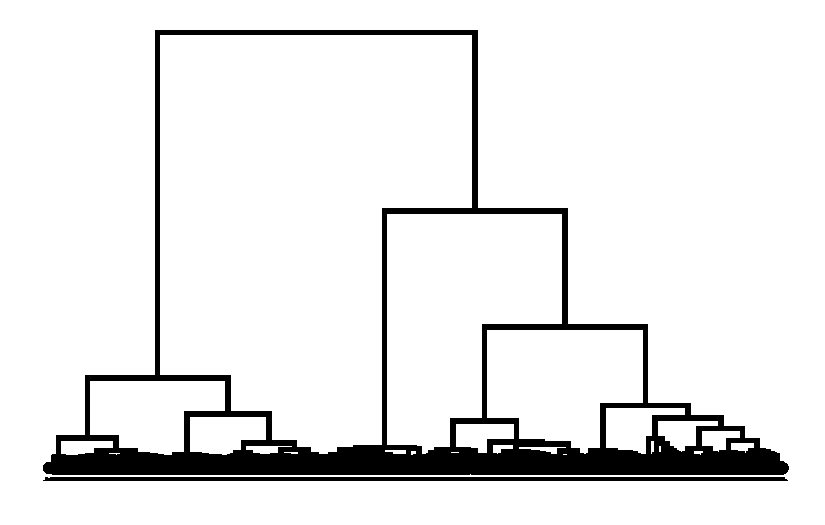
\includegraphics[width=1\textwidth,height=\textheight]{index_files/figure-pdf/unnamed-chunk-39-1.pdf}

}

\end{figure}

The following is the MDS for the Munkres similarity:

\begin{Shaded}
\begin{Highlighting}[]
\DocumentationTok{\#\# Metric multidimensional scaling}
\NormalTok{mds7 }\OtherTok{\textless{}{-}} \FunctionTok{cmdscale}\NormalTok{(}\FunctionTok{sqrt}\NormalTok{(}\DecValTok{1}\SpecialCharTok{{-}}\NormalTok{Sim\_Mun\_mDAG}\SpecialCharTok{\^{}}\DecValTok{2}\NormalTok{),}\AttributeTok{k=}\DecValTok{7}\NormalTok{,}\AttributeTok{eig=}\ConstantTok{TRUE}\NormalTok{)}
\NormalTok{mds7}\SpecialCharTok{$}\NormalTok{GOF}
\end{Highlighting}
\end{Shaded}

\begin{verbatim}
[1] 0.5605691 0.5800736
\end{verbatim}

\begin{Shaded}
\begin{Highlighting}[]
\NormalTok{mds }\OtherTok{\textless{}{-}}\NormalTok{ mds7}\SpecialCharTok{$}\NormalTok{points }\SpecialCharTok{\%\textgreater{}\%}  \FunctionTok{as\_tibble}\NormalTok{()}
\FunctionTok{colnames}\NormalTok{(mds) }\OtherTok{\textless{}{-}}\FunctionTok{paste0}\NormalTok{(}\StringTok{"Dim."}\NormalTok{,}\DecValTok{1}\SpecialCharTok{:}\FunctionTok{dim}\NormalTok{(mds7}\SpecialCharTok{$}\NormalTok{points)[}\DecValTok{2}\NormalTok{])}

\NormalTok{cooordinates}\OtherTok{=}\FunctionTok{as\_tibble}\NormalTok{(mds7}\SpecialCharTok{$}\NormalTok{points)}
\FunctionTok{colnames}\NormalTok{(cooordinates)}\OtherTok{=}\FunctionTok{paste}\NormalTok{(}\StringTok{"Component"}\NormalTok{,}\DecValTok{1}\SpecialCharTok{:}\DecValTok{7}\NormalTok{)}
\FunctionTok{ggpairs}\NormalTok{(cooordinates,}\AttributeTok{columns=}\DecValTok{1}\SpecialCharTok{:}\DecValTok{4}\NormalTok{,}
        \FunctionTok{aes}\NormalTok{(}\AttributeTok{color=}\NormalTok{meta\_taxo}\SpecialCharTok{$}\NormalTok{Kingdom[}\DecValTok{1}\SpecialCharTok{:}\DecValTok{884}\NormalTok{],}
            \AttributeTok{title=}\StringTok{"MDS 4 dimensions projection"}\NormalTok{,}\AttributeTok{legend=}\DecValTok{1}\NormalTok{),}
        \AttributeTok{lower=}\FunctionTok{list}\NormalTok{(}\AttributeTok{continuous=}\StringTok{"points"}\NormalTok{)) }\SpecialCharTok{+} 
  \FunctionTok{scale\_fill\_manual}\NormalTok{(}\AttributeTok{values =}\NormalTok{ colorsK}\SpecialCharTok{$}\NormalTok{Kingdom) }\SpecialCharTok{+} 
  \FunctionTok{theme}\NormalTok{(}\AttributeTok{legend.position =} \StringTok{"left"}\NormalTok{)}
\end{Highlighting}
\end{Shaded}

\begin{figure}[H]

{\centering 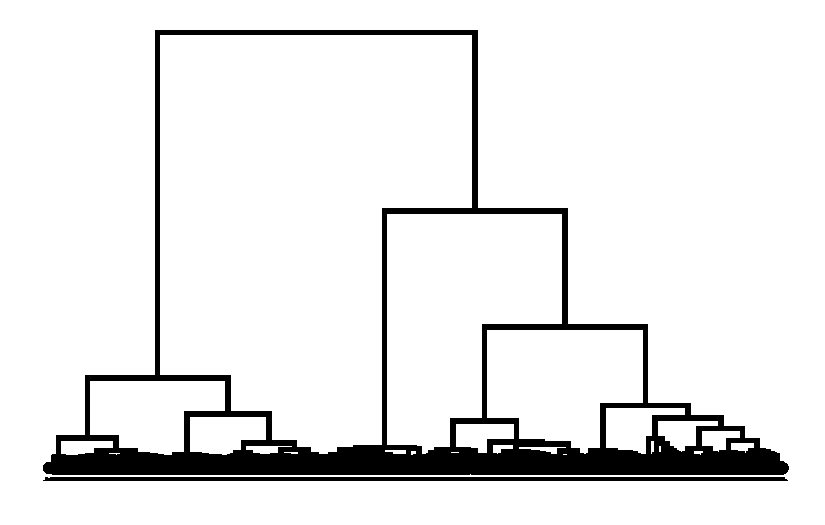
\includegraphics[width=1\textwidth,height=\textheight]{index_files/figure-pdf/unnamed-chunk-40-1.pdf}

}

\end{figure}

\hypertarget{hierarchical-clustering-msa-similarity}{%
\section{Hierarchical clustering MSA
similarity}\label{hierarchical-clustering-msa-similarity}}

We obtain a classification of the m-DAGs into different clusters as
follows:

\begin{Shaded}
\begin{Highlighting}[]
\NormalTok{D}\OtherTok{=}\FunctionTok{as.dist}\NormalTok{(}\FunctionTok{sqrt}\NormalTok{(}\DecValTok{1}\SpecialCharTok{{-}}\NormalTok{Sim\_MSA\_mDAG}\SpecialCharTok{\^{}}\DecValTok{2}\NormalTok{))}
\NormalTok{hc\_MSA}\OtherTok{=}\FunctionTok{hclust}\NormalTok{(}\FunctionTok{as.dist}\NormalTok{(D),}\AttributeTok{method =}\StringTok{"ward.D"}\NormalTok{)}
\NormalTok{clust4\_MSA}\OtherTok{=}\FunctionTok{cutree}\NormalTok{(hc\_MSA,}\DecValTok{4}\NormalTok{)}
\FunctionTok{table}\NormalTok{(clust4\_MSA,meta\_taxo}\SpecialCharTok{$}\NormalTok{Kingdom[}\DecValTok{1}\SpecialCharTok{:}\DecValTok{884}\NormalTok{])}
\end{Highlighting}
\end{Shaded}

\begin{verbatim}
          
clust4_MSA Animals Fungi Plants Protists
         1     331     0      0        0
         2     197     0      0        0
         3       7   154     14       56
         4       0     0    125        0
\end{verbatim}

\begin{Shaded}
\begin{Highlighting}[]
\NormalTok{clust5\_MSA}\OtherTok{=}\FunctionTok{cutree}\NormalTok{(hc\_MSA,}\DecValTok{5}\NormalTok{)}
\FunctionTok{table}\NormalTok{(clust5\_MSA,meta\_taxo}\SpecialCharTok{$}\NormalTok{Kingdom[}\DecValTok{1}\SpecialCharTok{:}\DecValTok{884}\NormalTok{])}
\end{Highlighting}
\end{Shaded}

\begin{verbatim}
          
clust5_MSA Animals Fungi Plants Protists
         1     129     0      0        0
         2     202     0      0        0
         3     197     0      0        0
         4       7   154     14       56
         5       0     0    125        0
\end{verbatim}

\begin{Shaded}
\begin{Highlighting}[]
\NormalTok{clust6\_MSA}\OtherTok{=}\FunctionTok{cutree}\NormalTok{(hc\_MSA,}\DecValTok{6}\NormalTok{)}
\FunctionTok{table}\NormalTok{(clust6\_MSA,meta\_taxo}\SpecialCharTok{$}\NormalTok{Kingdom[}\DecValTok{1}\SpecialCharTok{:}\DecValTok{884}\NormalTok{])}
\end{Highlighting}
\end{Shaded}

\begin{verbatim}
          
clust6_MSA Animals Fungi Plants Protists
         1     129     0      0        0
         2     202     0      0        0
         3     197     0      0        0
         4       7   149     14       34
         5       0     5      0       22
         6       0     0    125        0
\end{verbatim}

We can also create a table that correlates the clusters (in this case,
two clusters) with the Phylum classification:

\begin{Shaded}
\begin{Highlighting}[]
\NormalTok{aux}\OtherTok{=}\NormalTok{meta\_taxo[}\DecValTok{1}\SpecialCharTok{:}\DecValTok{884}\NormalTok{,] }\SpecialCharTok{\%\textgreater{}\%}
  \FunctionTok{select}\NormalTok{(Organism,Kingdom,Phylum,Class,Full\_Name)}
\NormalTok{aux}\SpecialCharTok{$}\NormalTok{clust4\_MSA}\OtherTok{=}\NormalTok{clust4\_MSA}
\NormalTok{aux\_Animals\_cluster\_1\_2 }\OtherTok{=}\NormalTok{ aux }\SpecialCharTok{\%\textgreater{}\%}
  \FunctionTok{filter}\NormalTok{(Kingdom}\SpecialCharTok{==}\StringTok{"Animals"}\NormalTok{,clust4\_MSA }\SpecialCharTok{\%in\%} \FunctionTok{c}\NormalTok{(}\DecValTok{1}\NormalTok{,}\DecValTok{2}\NormalTok{))}

\FunctionTok{table}\NormalTok{(aux\_Animals\_cluster\_1\_2}\SpecialCharTok{$}\NormalTok{Phylum,aux\_Animals\_cluster\_1\_2}\SpecialCharTok{$}\NormalTok{clust4\_MSA)}
\end{Highlighting}
\end{Shaded}

\begin{verbatim}
                  
                     1   2
  Annelids           0   1
  Arthropods         0 158
  Brachiopodas       0   1
  Cephalochordates   0   2
  Cnidarians         0  10
  Echinoderms        0   3
  Hemichordates      0   1
  Mollusks           0  14
  Nematodes          0   3
  Placozoans         0   1
  Poriferans         0   1
  Tunicates          0   2
  Vertebrates      331   0
\end{verbatim}

We can retrieve the information of the elements belonging to a specific
classification (Animals) that are part of a particular cluster as
follows:

\begin{Shaded}
\begin{Highlighting}[]
\NormalTok{aux\_7\_Animals\_cluster\_3}\OtherTok{=} \FunctionTok{filter}\NormalTok{(aux,}
\NormalTok{                                clust4\_MSA}\SpecialCharTok{==}\DecValTok{3}\NormalTok{,}
\NormalTok{                                Kingdom}\SpecialCharTok{==}\StringTok{"Animals"}\NormalTok{)}
\NormalTok{aux\_7\_Animals\_cluster\_3}
\end{Highlighting}
\end{Shaded}

\begin{verbatim}
# A tibble: 7 x 6
  Organism Kingdom Phylum    Class     Full_Name                      clust4_MSA
  <chr>    <chr>   <chr>     <chr>     <chr>                               <int>
1 bmy      Animals Nematodes Nematodes Brugia malayi (filaria)                 3
2 loa      Animals Nematodes Nematodes Loa loa (eye worm)                      3
3 tsp      Animals Nematodes Nematodes Trichinella spiralis                    3
4 egl      Animals Flatworms Flatworms Echinococcus granulosus (hyda~          3
5 ovi      Animals Flatworms Flatworms Opisthorchis viverrini (South~          3
6 shx      Animals Flatworms Flatworms Schistosoma haematobium (urin~          3
7 smm      Animals Flatworms Flatworms Schistosoma mansoni                     3
\end{verbatim}

\begin{Shaded}
\begin{Highlighting}[]
\NormalTok{aux\_14\_Plants\_clust2}\OtherTok{=} \FunctionTok{filter}\NormalTok{(aux,clust4\_MSA}\SpecialCharTok{==}\DecValTok{3}\NormalTok{,}
\NormalTok{                             Kingdom}\SpecialCharTok{==}\StringTok{"Plants"}\NormalTok{)}
\NormalTok{aux\_14\_Plants\_clust2}
\end{Highlighting}
\end{Shaded}

\begin{verbatim}
# A tibble: 14 x 6
   Organism Kingdom Phylum Class Full_Name                      clust4_MSA
   <chr>    <chr>   <chr>  <chr> <chr>                               <int>
 1 apro     Plants  Green  algae Auxenochlorella protothecoides          3
 2 bpg      Plants  Green  algae Bathycoccus prasinos                    3
 3 cre      Plants  Green  algae Chlamydomonas reinhardtii               3
 4 csl      Plants  Green  algae Coccomyxa subellipsoidea                3
 5 cvr      Plants  Green  algae Chlorella variabilis                    3
 6 mis      Plants  Green  algae Micromonas commoda                      3
 7 mng      Plants  Green  algae Monoraphidium neglectum                 3
 8 mpp      Plants  Green  algae Micromonas pusilla                      3
 9 olu      Plants  Green  algae Ostreococcus lucimarinus                3
10 ota      Plants  Green  algae Ostreococcus tauri                      3
11 vcn      Plants  Green  algae Volvox carteri f. nagariensis           3
12 ccp      Plants  Red    algae Chondrus crispus (carragheen)           3
13 cme      Plants  Red    algae Cyanidioschyzon merolae                 3
14 gsl      Plants  Red    algae Galdieria sulphuraria                   3
\end{verbatim}

\begin{Shaded}
\begin{Highlighting}[]
\NormalTok{aux\_all\_algae\_class}\OtherTok{=}\NormalTok{ aux }\SpecialCharTok{\%\textgreater{}\%} 
  \FunctionTok{filter}\NormalTok{(Kingdom}\SpecialCharTok{==}\StringTok{"Plants"}\NormalTok{,}
\NormalTok{         Class }\SpecialCharTok{\%in\%} \FunctionTok{c}\NormalTok{(}\StringTok{"algae"}\NormalTok{))}
\NormalTok{aux\_all\_algae\_class}
\end{Highlighting}
\end{Shaded}

\begin{verbatim}
# A tibble: 14 x 6
   Organism Kingdom Phylum Class Full_Name                      clust4_MSA
   <chr>    <chr>   <chr>  <chr> <chr>                               <int>
 1 apro     Plants  Green  algae Auxenochlorella protothecoides          3
 2 bpg      Plants  Green  algae Bathycoccus prasinos                    3
 3 cre      Plants  Green  algae Chlamydomonas reinhardtii               3
 4 csl      Plants  Green  algae Coccomyxa subellipsoidea                3
 5 cvr      Plants  Green  algae Chlorella variabilis                    3
 6 mis      Plants  Green  algae Micromonas commoda                      3
 7 mng      Plants  Green  algae Monoraphidium neglectum                 3
 8 mpp      Plants  Green  algae Micromonas pusilla                      3
 9 olu      Plants  Green  algae Ostreococcus lucimarinus                3
10 ota      Plants  Green  algae Ostreococcus tauri                      3
11 vcn      Plants  Green  algae Volvox carteri f. nagariensis           3
12 ccp      Plants  Red    algae Chondrus crispus (carragheen)           3
13 cme      Plants  Red    algae Cyanidioschyzon merolae                 3
14 gsl      Plants  Red    algae Galdieria sulphuraria                   3
\end{verbatim}

We can retrieve the information of the elements from a specific Phylum
or Class, and the cluster they belong to, as follows:

\begin{Shaded}
\begin{Highlighting}[]
\NormalTok{aux\_all\_Nematodes\_Flatworns}\OtherTok{=}\NormalTok{ aux }\SpecialCharTok{\%\textgreater{}\%} 
  \FunctionTok{filter}\NormalTok{(Kingdom}\SpecialCharTok{==}\StringTok{"Animals"}\NormalTok{,}
\NormalTok{         Phylum }\SpecialCharTok{\%in\%} \FunctionTok{c}\NormalTok{(}\StringTok{"Nematodes"}\NormalTok{,}\StringTok{"Flatworms"}\NormalTok{))}
\NormalTok{aux\_all\_Nematodes\_Flatworns}
\end{Highlighting}
\end{Shaded}

\begin{verbatim}
# A tibble: 10 x 6
   Organism Kingdom Phylum    Class     Full_Name                     clust4_MSA
   <chr>    <chr>   <chr>     <chr>     <chr>                              <int>
 1 bmy      Animals Nematodes Nematodes Brugia malayi (filaria)                3
 2 cbr      Animals Nematodes Nematodes Caenorhabditis briggsae (nem~          2
 3 cel      Animals Nematodes Nematodes Caenorhabditis elegans (nema~          2
 4 loa      Animals Nematodes Nematodes Loa loa (eye worm)                     3
 5 nai      Animals Nematodes Nematodes Necator americanus (New Worl~          2
 6 tsp      Animals Nematodes Nematodes Trichinella spiralis                   3
 7 egl      Animals Flatworms Flatworms Echinococcus granulosus (hyd~          3
 8 ovi      Animals Flatworms Flatworms Opisthorchis viverrini (Sout~          3
 9 shx      Animals Flatworms Flatworms Schistosoma haematobium (uri~          3
10 smm      Animals Flatworms Flatworms Schistosoma mansoni                    3
\end{verbatim}

\hypertarget{hierarchical-clustering-munkres-similarity}{%
\section{Hierarchical clustering Munkres
similarity}\label{hierarchical-clustering-munkres-similarity}}

We obtain a classification of the m-DAGs into different clusters and
retrieve the cluster's information as follows:

\begin{Shaded}
\begin{Highlighting}[]
\NormalTok{D}\OtherTok{=}\FunctionTok{as.dist}\NormalTok{(}\FunctionTok{sqrt}\NormalTok{(}\DecValTok{1}\SpecialCharTok{{-}}\NormalTok{Sim\_Mun\_mDAG}\SpecialCharTok{\^{}}\DecValTok{2}\NormalTok{))}
\NormalTok{hc\_Mun}\OtherTok{=}\FunctionTok{hclust}\NormalTok{(}\FunctionTok{as.dist}\NormalTok{(D),}\AttributeTok{method =}\StringTok{"ward.D"}\NormalTok{)}
\end{Highlighting}
\end{Shaded}

\begin{Shaded}
\begin{Highlighting}[]
\NormalTok{clust4\_Mun}\OtherTok{=}\FunctionTok{cutree}\NormalTok{(hc\_Mun,}\DecValTok{4}\NormalTok{)}
\FunctionTok{table}\NormalTok{(clust4\_Mun,meta\_taxo}\SpecialCharTok{$}\NormalTok{Kingdom[}\DecValTok{1}\SpecialCharTok{:}\DecValTok{884}\NormalTok{])}
\end{Highlighting}
\end{Shaded}

\begin{verbatim}
          
clust4_Mun Animals Fungi Plants Protists
         1     331     0      0        0
         2     197     0      0        0
         3       7   154     14       56
         4       0     0    125        0
\end{verbatim}

\begin{Shaded}
\begin{Highlighting}[]
\NormalTok{aux}\OtherTok{=}\NormalTok{meta\_taxo[}\DecValTok{1}\SpecialCharTok{:}\DecValTok{884}\NormalTok{,] }\SpecialCharTok{\%\textgreater{}\%}
  \FunctionTok{select}\NormalTok{(Organism,Kingdom,Phylum,Class,Full\_Name)}
\NormalTok{aux}\SpecialCharTok{$}\NormalTok{clust4\_Mun}\OtherTok{=}\NormalTok{clust4\_Mun}
\NormalTok{aux\_Animals\_cluster\_1\_2\_Mun }\OtherTok{=}\NormalTok{ aux }\SpecialCharTok{\%\textgreater{}\%}
  \FunctionTok{filter}\NormalTok{(Kingdom}\SpecialCharTok{==}\StringTok{"Animals"}\NormalTok{,clust4\_Mun }\SpecialCharTok{\%in\%} \FunctionTok{c}\NormalTok{(}\DecValTok{1}\NormalTok{,}\DecValTok{2}\NormalTok{))}

\FunctionTok{table}\NormalTok{(aux\_Animals\_cluster\_1\_2\_Mun}\SpecialCharTok{$}\NormalTok{Phylum,}
\NormalTok{      aux\_Animals\_cluster\_1\_2\_Mun}\SpecialCharTok{$}\NormalTok{clust4\_Mun)}
\end{Highlighting}
\end{Shaded}

\begin{verbatim}
                  
                     1   2
  Annelids           0   1
  Arthropods         0 158
  Brachiopodas       0   1
  Cephalochordates   0   2
  Cnidarians         0  10
  Echinoderms        0   3
  Hemichordates      0   1
  Mollusks           0  14
  Nematodes          0   3
  Placozoans         0   1
  Poriferans         0   1
  Tunicates          0   2
  Vertebrates      331   0
\end{verbatim}

\begin{Shaded}
\begin{Highlighting}[]
\NormalTok{aux\_7\_Animals\_cluster\_3\_Mun}\OtherTok{=} \FunctionTok{filter}\NormalTok{(aux,}
\NormalTok{                                clust4\_Mun}\SpecialCharTok{==}\DecValTok{3}\NormalTok{,}
\NormalTok{                                Kingdom}\SpecialCharTok{==}\StringTok{"Animals"}\NormalTok{)}
\NormalTok{aux\_7\_Animals\_cluster\_3\_Mun}
\end{Highlighting}
\end{Shaded}

\begin{verbatim}
# A tibble: 7 x 6
  Organism Kingdom Phylum    Class     Full_Name                      clust4_Mun
  <chr>    <chr>   <chr>     <chr>     <chr>                               <int>
1 bmy      Animals Nematodes Nematodes Brugia malayi (filaria)                 3
2 loa      Animals Nematodes Nematodes Loa loa (eye worm)                      3
3 tsp      Animals Nematodes Nematodes Trichinella spiralis                    3
4 egl      Animals Flatworms Flatworms Echinococcus granulosus (hyda~          3
5 ovi      Animals Flatworms Flatworms Opisthorchis viverrini (South~          3
6 shx      Animals Flatworms Flatworms Schistosoma haematobium (urin~          3
7 smm      Animals Flatworms Flatworms Schistosoma mansoni                     3
\end{verbatim}

\begin{Shaded}
\begin{Highlighting}[]
\NormalTok{aux\_all\_Nematodes\_Flatworns}\OtherTok{=}\NormalTok{ aux }\SpecialCharTok{\%\textgreater{}\%} 
  \FunctionTok{filter}\NormalTok{(Kingdom}\SpecialCharTok{==}\StringTok{"Animals"}\NormalTok{,}
\NormalTok{         Phylum }\SpecialCharTok{\%in\%} \FunctionTok{c}\NormalTok{(}\StringTok{"Nematodes"}\NormalTok{,}\StringTok{"Flatworms"}\NormalTok{))}
\NormalTok{aux\_all\_Nematodes\_Flatworns}
\end{Highlighting}
\end{Shaded}

\begin{verbatim}
# A tibble: 10 x 6
   Organism Kingdom Phylum    Class     Full_Name                     clust4_Mun
   <chr>    <chr>   <chr>     <chr>     <chr>                              <int>
 1 bmy      Animals Nematodes Nematodes Brugia malayi (filaria)                3
 2 cbr      Animals Nematodes Nematodes Caenorhabditis briggsae (nem~          2
 3 cel      Animals Nematodes Nematodes Caenorhabditis elegans (nema~          2
 4 loa      Animals Nematodes Nematodes Loa loa (eye worm)                     3
 5 nai      Animals Nematodes Nematodes Necator americanus (New Worl~          2
 6 tsp      Animals Nematodes Nematodes Trichinella spiralis                   3
 7 egl      Animals Flatworms Flatworms Echinococcus granulosus (hyd~          3
 8 ovi      Animals Flatworms Flatworms Opisthorchis viverrini (Sout~          3
 9 shx      Animals Flatworms Flatworms Schistosoma haematobium (uri~          3
10 smm      Animals Flatworms Flatworms Schistosoma mansoni                    3
\end{verbatim}

\begin{Shaded}
\begin{Highlighting}[]
\NormalTok{aux\_14\_Plants\_clust2\_Mun}\OtherTok{=} \FunctionTok{filter}\NormalTok{(aux,clust4\_Mun}\SpecialCharTok{==}\DecValTok{3}\NormalTok{,}
\NormalTok{                             Kingdom}\SpecialCharTok{==}\StringTok{"Plants"}\NormalTok{)}
\NormalTok{aux\_14\_Plants\_clust2\_Mun}
\end{Highlighting}
\end{Shaded}

\begin{verbatim}
# A tibble: 14 x 6
   Organism Kingdom Phylum Class Full_Name                      clust4_Mun
   <chr>    <chr>   <chr>  <chr> <chr>                               <int>
 1 apro     Plants  Green  algae Auxenochlorella protothecoides          3
 2 bpg      Plants  Green  algae Bathycoccus prasinos                    3
 3 cre      Plants  Green  algae Chlamydomonas reinhardtii               3
 4 csl      Plants  Green  algae Coccomyxa subellipsoidea                3
 5 cvr      Plants  Green  algae Chlorella variabilis                    3
 6 mis      Plants  Green  algae Micromonas commoda                      3
 7 mng      Plants  Green  algae Monoraphidium neglectum                 3
 8 mpp      Plants  Green  algae Micromonas pusilla                      3
 9 olu      Plants  Green  algae Ostreococcus lucimarinus                3
10 ota      Plants  Green  algae Ostreococcus tauri                      3
11 vcn      Plants  Green  algae Volvox carteri f. nagariensis           3
12 ccp      Plants  Red    algae Chondrus crispus (carragheen)           3
13 cme      Plants  Red    algae Cyanidioschyzon merolae                 3
14 gsl      Plants  Red    algae Galdieria sulphuraria                   3
\end{verbatim}

\begin{Shaded}
\begin{Highlighting}[]
\NormalTok{aux\_all\_algae\_class}\OtherTok{=}\NormalTok{ aux }\SpecialCharTok{\%\textgreater{}\%} 
  \FunctionTok{filter}\NormalTok{(Kingdom}\SpecialCharTok{==}\StringTok{"Plants"}\NormalTok{,}
\NormalTok{         Class }\SpecialCharTok{\%in\%} \FunctionTok{c}\NormalTok{(}\StringTok{"algae"}\NormalTok{))}
\NormalTok{aux\_all\_algae\_class}
\end{Highlighting}
\end{Shaded}

\begin{verbatim}
# A tibble: 14 x 6
   Organism Kingdom Phylum Class Full_Name                      clust4_Mun
   <chr>    <chr>   <chr>  <chr> <chr>                               <int>
 1 apro     Plants  Green  algae Auxenochlorella protothecoides          3
 2 bpg      Plants  Green  algae Bathycoccus prasinos                    3
 3 cre      Plants  Green  algae Chlamydomonas reinhardtii               3
 4 csl      Plants  Green  algae Coccomyxa subellipsoidea                3
 5 cvr      Plants  Green  algae Chlorella variabilis                    3
 6 mis      Plants  Green  algae Micromonas commoda                      3
 7 mng      Plants  Green  algae Monoraphidium neglectum                 3
 8 mpp      Plants  Green  algae Micromonas pusilla                      3
 9 olu      Plants  Green  algae Ostreococcus lucimarinus                3
10 ota      Plants  Green  algae Ostreococcus tauri                      3
11 vcn      Plants  Green  algae Volvox carteri f. nagariensis           3
12 ccp      Plants  Red    algae Chondrus crispus (carragheen)           3
13 cme      Plants  Red    algae Cyanidioschyzon merolae                 3
14 gsl      Plants  Red    algae Galdieria sulphuraria                   3
\end{verbatim}

\hypertarget{comparison-between-msa-and-munkres-similarities}{%
\section{Comparison between MSA and Munkres
similarities}\label{comparison-between-msa-and-munkres-similarities}}

In order to compare the two similarities we consider the Spearman and
Pearson correlation. First, we load the similarities for every pair of
m-DAG and each similarity measure.

\begin{Shaded}
\begin{Highlighting}[]
\NormalTok{n}\OtherTok{=}\FunctionTok{length}\NormalTok{(meta\_taxo}\SpecialCharTok{$}\NormalTok{mDAG\_Id[}\DecValTok{1}\SpecialCharTok{:}\DecValTok{884}\NormalTok{])}
\NormalTok{n}
\end{Highlighting}
\end{Shaded}

\begin{verbatim}
[1] 884
\end{verbatim}

\begin{Shaded}
\begin{Highlighting}[]
\FunctionTok{dim}\NormalTok{(Sim\_MSA\_mDAG)}
\end{Highlighting}
\end{Shaded}

\begin{verbatim}
[1] 884 884
\end{verbatim}

\begin{Shaded}
\begin{Highlighting}[]
\NormalTok{aux}\OtherTok{=}\FunctionTok{as\_tibble}\NormalTok{(Sim\_MSA\_mDAG)}
\NormalTok{aux}\SpecialCharTok{$}\NormalTok{mDag}\OtherTok{=}\FunctionTok{names}\NormalTok{(aux)}
\NormalTok{aux}\OtherTok{=}\NormalTok{aux }\SpecialCharTok{\%\textgreater{}\%} \FunctionTok{pivot\_longer}\NormalTok{(}\AttributeTok{cols=}\StringTok{\textasciigrave{}}\AttributeTok{0313}\StringTok{\textasciigrave{}}\SpecialCharTok{:}\StringTok{\textasciigrave{}}\AttributeTok{0300}\StringTok{\textasciigrave{}}\NormalTok{,}
                         \AttributeTok{names\_to=}\StringTok{"mDag\_2"}\NormalTok{,}
                         \AttributeTok{values\_to=}\StringTok{"Sim\_MSA"}\NormalTok{)}

\NormalTok{aux\_2}\OtherTok{=}\NormalTok{ aux }\SpecialCharTok{\%\textgreater{}\%}  \FunctionTok{mutate}\NormalTok{(}\AttributeTok{i=}\FunctionTok{pmax}\NormalTok{(}\FunctionTok{as.integer}\NormalTok{(mDag),}
                              \FunctionTok{as.integer}\NormalTok{(mDag\_2)),}
                       \AttributeTok{j=}\FunctionTok{pmin}\NormalTok{(}\FunctionTok{as.integer}\NormalTok{(mDag),}
                       \FunctionTok{as.integer}\NormalTok{(mDag\_2))) }\SpecialCharTok{\%\textgreater{}\%} \FunctionTok{unite}\NormalTok{(}\StringTok{"ij"}\NormalTok{,i}\SpecialCharTok{:}\NormalTok{j) }\SpecialCharTok{\%\textgreater{}\%}
  \FunctionTok{filter}\NormalTok{(}\FunctionTok{duplicated}\NormalTok{(ij))}


\NormalTok{aux}\OtherTok{=}\FunctionTok{as\_tibble}\NormalTok{(Sim\_Mun\_mDAG)}
\NormalTok{aux}\SpecialCharTok{$}\NormalTok{mDag}\OtherTok{=}\FunctionTok{names}\NormalTok{(aux)}
\NormalTok{aux}\OtherTok{=}\NormalTok{aux }\SpecialCharTok{\%\textgreater{}\%} \FunctionTok{pivot\_longer}\NormalTok{(}\AttributeTok{cols=}\StringTok{\textasciigrave{}}\AttributeTok{0313}\StringTok{\textasciigrave{}}\SpecialCharTok{:}\StringTok{\textasciigrave{}}\AttributeTok{0300}\StringTok{\textasciigrave{}}\NormalTok{,}
                         \AttributeTok{names\_to=}\StringTok{"mDag\_2"}\NormalTok{,}
                         \AttributeTok{values\_to=}\StringTok{"Sim\_Mun"}\NormalTok{)}
\NormalTok{aux\_2 }\OtherTok{=}\NormalTok{ aux\_2 }\SpecialCharTok{\%\textgreater{}\%} \FunctionTok{left\_join}\NormalTok{(aux)}

\NormalTok{Sim\_comp}\OtherTok{=}\NormalTok{aux\_2}
\FunctionTok{rm}\NormalTok{(aux,aux\_2)}
\end{Highlighting}
\end{Shaded}

Next we obtain the Spearman and Pearson correlations as follows:

\begin{Shaded}
\begin{Highlighting}[]
\FunctionTok{cor}\NormalTok{(Sim\_comp[,}\FunctionTok{c}\NormalTok{(}\DecValTok{3}\NormalTok{,}\DecValTok{5}\NormalTok{)],}\AttributeTok{method=}\StringTok{"spearman"}\NormalTok{)}
\end{Highlighting}
\end{Shaded}

\begin{verbatim}
          Sim_MSA   Sim_Mun
Sim_MSA 1.0000000 0.8930995
Sim_Mun 0.8930995 1.0000000
\end{verbatim}

\begin{Shaded}
\begin{Highlighting}[]
\FunctionTok{cor}\NormalTok{(Sim\_comp[,}\FunctionTok{c}\NormalTok{(}\DecValTok{3}\NormalTok{,}\DecValTok{5}\NormalTok{)],}\AttributeTok{method=}\StringTok{"pearson"}\NormalTok{)}
\end{Highlighting}
\end{Shaded}

\begin{verbatim}
          Sim_MSA   Sim_Mun
Sim_MSA 1.0000000 0.9203871
Sim_Mun 0.9203871 1.0000000
\end{verbatim}

\begin{Shaded}
\begin{Highlighting}[]
\NormalTok{GGally}\SpecialCharTok{::}\FunctionTok{ggpairs}\NormalTok{(Sim\_comp[,}\FunctionTok{c}\NormalTok{(}\DecValTok{3}\NormalTok{,}\DecValTok{5}\NormalTok{)])}
\end{Highlighting}
\end{Shaded}

\begin{figure}[H]

{\centering 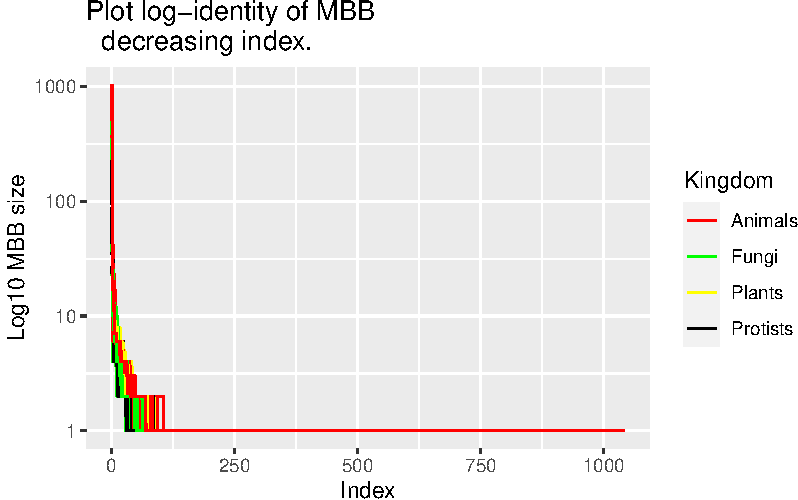
\includegraphics[width=1\textwidth,height=\textheight]{index_files/figure-pdf/unnamed-chunk-52-1.pdf}

}

\end{figure}

\begin{Shaded}
\begin{Highlighting}[]
\NormalTok{sim\_pairs}\OtherTok{=}\NormalTok{ Sim\_comp}\SpecialCharTok{\%\textgreater{}\%} \FunctionTok{pivot\_longer}\NormalTok{(}
  \AttributeTok{cols=}\FunctionTok{c}\NormalTok{(Sim\_MSA,Sim\_Mun),}
  \AttributeTok{names\_to=}\StringTok{"Method"}\NormalTok{,}
  \AttributeTok{values\_to=}\StringTok{"Similarity"}\NormalTok{)}

\NormalTok{ggstatsplot}\SpecialCharTok{::}\FunctionTok{ggbetweenstats}\NormalTok{(}
  \AttributeTok{data =}\NormalTok{ sim\_pairs,}
  \AttributeTok{x =}\NormalTok{ Method,}
  \AttributeTok{y =}\NormalTok{ Similarity,}
  \AttributeTok{centrality.plotting=}\ConstantTok{TRUE}\NormalTok{)}
\end{Highlighting}
\end{Shaded}

\begin{figure}[H]

{\centering 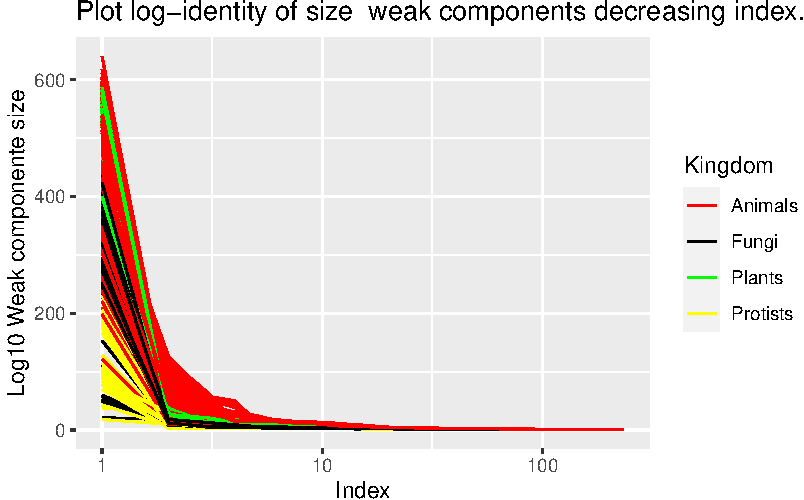
\includegraphics[width=1\textwidth,height=\textheight]{index_files/figure-pdf/unnamed-chunk-53-1.pdf}

}

\end{figure}

\begin{Shaded}
\begin{Highlighting}[]
\FunctionTok{library}\NormalTok{(hrbrthemes)}
\FunctionTok{library}\NormalTok{(viridis)}
\NormalTok{sim\_pairs }\SpecialCharTok{\%\textgreater{}\%}
  \FunctionTok{ggplot}\NormalTok{( }\FunctionTok{aes}\NormalTok{(}\AttributeTok{x=}\NormalTok{Method, }\AttributeTok{y=}\NormalTok{Similarity, }\AttributeTok{fill=}\NormalTok{Method)) }\SpecialCharTok{+}
  \FunctionTok{geom\_boxplot}\NormalTok{() }\SpecialCharTok{+}
  \FunctionTok{scale\_fill\_viridis}\NormalTok{(}\AttributeTok{discrete =} \ConstantTok{TRUE}\NormalTok{, }\AttributeTok{alpha=}\FloatTok{0.6}\NormalTok{) }\SpecialCharTok{+}
  \FunctionTok{theme}\NormalTok{(}\AttributeTok{legend.position=}\StringTok{"none"}\NormalTok{)}\SpecialCharTok{+}
  \FunctionTok{ggtitle}\NormalTok{(}\StringTok{"Boxplot diagram of the similaritires between the two aproaches"}\NormalTok{) }
\end{Highlighting}
\end{Shaded}

\begin{figure}[H]

{\centering 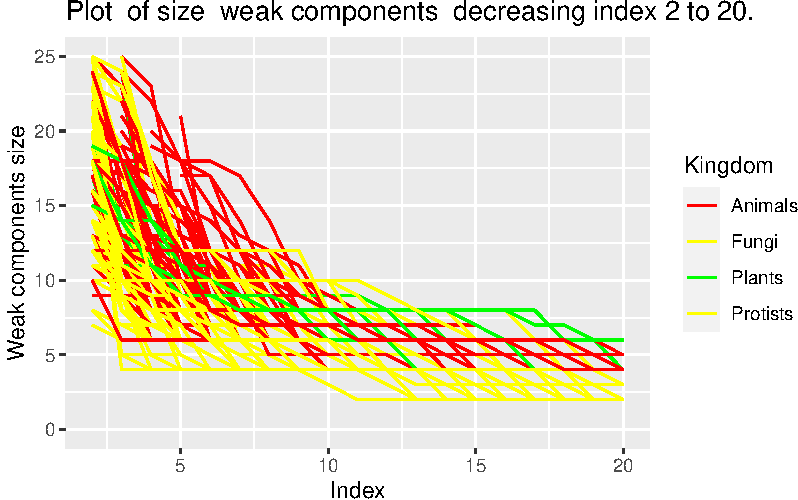
\includegraphics[width=1\textwidth,height=\textheight]{index_files/figure-pdf/unnamed-chunk-54-1.pdf}

}

\end{figure}

\bookmarksetup{startatroot}

\hypertarget{clusters-analysis}{%
\chapter{Clusters analysis}\label{clusters-analysis}}

In the Eukaryotes test, we aimed to analyze which factors caused some
algae and plants to be distinguished from their respective kingdoms. To
address this question, we revisited the core metabolism obtained with
MetaDAG, focusing on each cluster.

\begin{Shaded}
\begin{Highlighting}[]
\NormalTok{reactions}\OtherTok{=}\FunctionTok{names}\NormalTok{(Results)}
\NormalTok{reactions}\OtherTok{=}\NormalTok{reactions[}\FunctionTok{grep}\NormalTok{(}\StringTok{"(\^{}R}\SpecialCharTok{\textbackslash{}\textbackslash{}}\StringTok{d\{5\})"}\NormalTok{,reactions)]}
\NormalTok{reactions}\OtherTok{=}\FunctionTok{tibble}\NormalTok{(reactions)}
\NormalTok{reactions}\OtherTok{=}\NormalTok{reactions }\SpecialCharTok{\%\textgreater{}\%} \FunctionTok{separate}\NormalTok{(reactions, }\AttributeTok{into=}\FunctionTok{c}\NormalTok{(}\StringTok{"r\_id"}\NormalTok{,}\StringTok{"enzyme"}\NormalTok{),}\AttributeTok{sep=}\StringTok{"}\SpecialCharTok{\textbackslash{}\textbackslash{}}\StringTok{("}\NormalTok{,}\AttributeTok{remove=}\ConstantTok{FALSE}\NormalTok{)}
\NormalTok{reactions}\OtherTok{=}\NormalTok{reactions }\SpecialCharTok{\%\textgreater{}\%} \FunctionTok{mutate}\NormalTok{(}\AttributeTok{enzyme=}\FunctionTok{gsub}\NormalTok{(}\StringTok{"}\SpecialCharTok{\textbackslash{}\textbackslash{}}\StringTok{(|}\SpecialCharTok{\textbackslash{}\textbackslash{}}\StringTok{)"}\NormalTok{,}\StringTok{""}\NormalTok{,enzyme))}
\CommentTok{\#reactions=reactions[,{-}3]}
\NormalTok{reactions}\SpecialCharTok{$}\NormalTok{rev}\OtherTok{=}\NormalTok{stringr}\SpecialCharTok{::}\FunctionTok{str\_detect}\NormalTok{(reactions}\SpecialCharTok{$}\NormalTok{r\_id,}\StringTok{"v"}\NormalTok{)}
\end{Highlighting}
\end{Shaded}

The results of the clusters are compared to the classification of
Kingdoms for both similarity measures:

\begin{Shaded}
\begin{Highlighting}[]
\NormalTok{clust4\_MSA2}\OtherTok{=}\FunctionTok{tibble}\NormalTok{(}\AttributeTok{mDAG\_Id=}\FunctionTok{names}\NormalTok{(clust4\_MSA), }\AttributeTok{clust4\_MSA=}\NormalTok{clust4\_MSA)}
\NormalTok{clust4\_Mun2}\OtherTok{=}\FunctionTok{tibble}\NormalTok{(}\AttributeTok{mDAG\_Id=}\FunctionTok{names}\NormalTok{(clust4\_Mun), }\AttributeTok{clust4\_Mun=}\NormalTok{clust4\_Mun)}
\NormalTok{meta\_taxo2}\OtherTok{=}\NormalTok{meta\_taxo}
\NormalTok{meta\_taxo2}\OtherTok{=}\NormalTok{meta\_taxo2 }\SpecialCharTok{\%\textgreater{}\%} \FunctionTok{left\_join}\NormalTok{(clust4\_MSA2,}\AttributeTok{by=} \StringTok{"mDAG\_Id"}\NormalTok{) }\SpecialCharTok{\%\textgreater{}\%} 
  \FunctionTok{left\_join}\NormalTok{(clust4\_Mun2,}\AttributeTok{by=} \StringTok{"mDAG\_Id"}\NormalTok{)}
\NormalTok{meta\_taxo2}\SpecialCharTok{$}\NormalTok{combined\_cluster\_MSA\_Kingdom}\OtherTok{=}\FunctionTok{paste0}\NormalTok{(meta\_taxo2}\SpecialCharTok{$}\NormalTok{Kingdom,meta\_taxo2}\SpecialCharTok{$}\NormalTok{clust4\_MSA)}
\NormalTok{meta\_taxo2}\SpecialCharTok{$}\NormalTok{combined\_cluster\_Mun\_Kingdom}\OtherTok{=}\FunctionTok{paste0}\NormalTok{(meta\_taxo2}\SpecialCharTok{$}\NormalTok{Kingdom,meta\_taxo2}\SpecialCharTok{$}\NormalTok{clust4\_MSA)}
\FunctionTok{write.csv}\NormalTok{(meta\_taxo2,}\AttributeTok{file=}\StringTok{"meta\_taxo\_4\_clusters.csv"}\NormalTok{)}
\end{Highlighting}
\end{Shaded}

\begin{Shaded}
\begin{Highlighting}[]
\NormalTok{knitr}\SpecialCharTok{::}\FunctionTok{kable}\NormalTok{(}\FunctionTok{table}\NormalTok{(meta\_taxo2}\SpecialCharTok{$}\NormalTok{Kingdom,meta\_taxo2}\SpecialCharTok{$}\NormalTok{clust4\_MSA))}
\end{Highlighting}
\end{Shaded}

\begin{tabular}{l|r|r|r|r}
\hline
  & 1 & 2 & 3 & 4\\
\hline
Animals & 331 & 197 & 7 & 0\\
\hline
Fungi & 0 & 0 & 154 & 0\\
\hline
Plants & 0 & 0 & 14 & 125\\
\hline
Protists & 0 & 0 & 56 & 0\\
\hline
\end{tabular}

\begin{Shaded}
\begin{Highlighting}[]
\NormalTok{knitr}\SpecialCharTok{::}\FunctionTok{kable}\NormalTok{(}\FunctionTok{table}\NormalTok{(meta\_taxo2}\SpecialCharTok{$}\NormalTok{Kingdom,meta\_taxo2}\SpecialCharTok{$}\NormalTok{clust4\_Mun))}
\end{Highlighting}
\end{Shaded}

\begin{tabular}{l|r|r|r|r}
\hline
  & 1 & 2 & 3 & 4\\
\hline
Animals & 331 & 197 & 7 & 0\\
\hline
Fungi & 0 & 0 & 154 & 0\\
\hline
Plants & 0 & 0 & 14 & 125\\
\hline
Protists & 0 & 0 & 56 & 0\\
\hline
\end{tabular}

\begin{Shaded}
\begin{Highlighting}[]
\NormalTok{knitr}\SpecialCharTok{::}\FunctionTok{kable}\NormalTok{(}\FunctionTok{table}\NormalTok{(meta\_taxo2}\SpecialCharTok{$}\NormalTok{clust4\_Mun,meta\_taxo2}\SpecialCharTok{$}\NormalTok{clust4\_MSA))}
\end{Highlighting}
\end{Shaded}

\begin{tabular}{r|r|r|r}
\hline
1 & 2 & 3 & 4\\
\hline
331 & 0 & 0 & 0\\
\hline
0 & 197 & 0 & 0\\
\hline
0 & 0 & 231 & 0\\
\hline
0 & 0 & 0 & 125\\
\hline
\end{tabular}

The table below correlates the clusters with the Phylum information.

\begin{Shaded}
\begin{Highlighting}[]
\FunctionTok{library}\NormalTok{(reshape2)}
\NormalTok{MSA\_table}\OtherTok{=}\FunctionTok{melt}\NormalTok{(}\FunctionTok{table}\NormalTok{(meta\_taxo2}\SpecialCharTok{$}\NormalTok{Kingdom,meta\_taxo2}\SpecialCharTok{$}\NormalTok{Phylum,meta\_taxo2}\SpecialCharTok{$}\NormalTok{clust4\_MSA))}
\FunctionTok{names}\NormalTok{(MSA\_table)}\OtherTok{=}\FunctionTok{c}\NormalTok{(}\StringTok{"Kingdom"}\NormalTok{,}\StringTok{"Phylum"}\NormalTok{,}\StringTok{"cluster\_MSA"}\NormalTok{,}\StringTok{"N"}\NormalTok{)}
\NormalTok{MSA\_table}\OtherTok{=}\NormalTok{MSA\_table }\SpecialCharTok{\%\textgreater{}\%} \FunctionTok{filter}\NormalTok{(N}\SpecialCharTok{!=}\DecValTok{0}\NormalTok{)}
\end{Highlighting}
\end{Shaded}

\begin{Shaded}
\begin{Highlighting}[]
\NormalTok{knitr}\SpecialCharTok{::}\FunctionTok{kable}\NormalTok{(MSA\_table)}
\end{Highlighting}
\end{Shaded}

\begin{tabular}{l|l|r|r}
\hline
Kingdom & Phylum & cluster\_MSA & N\\
\hline
Animals & Vertebrates & 1 & 331\\
\hline
Animals & Annelids & 2 & 1\\
\hline
Animals & Arthropods & 2 & 158\\
\hline
Animals & Brachiopodas & 2 & 1\\
\hline
Animals & Cephalochordates & 2 & 2\\
\hline
Animals & Cnidarians & 2 & 10\\
\hline
Animals & Echinoderms & 2 & 3\\
\hline
Animals & Hemichordates & 2 & 1\\
\hline
Animals & Mollusks & 2 & 14\\
\hline
Animals & Nematodes & 2 & 3\\
\hline
Animals & Placozoans & 2 & 1\\
\hline
Animals & Poriferans & 2 & 1\\
\hline
Animals & Tunicates & 2 & 2\\
\hline
Protists & Alveolates & 3 & 25\\
\hline
Protists & Amoebozoa & 3 & 7\\
\hline
Fungi & Ascomycetes & 3 & 113\\
\hline
Fungi & Basidiomycetes & 3 & 36\\
\hline
Protists & Choanoflagellates & 3 & 2\\
\hline
Protists & Cryptomonads & 3 & 1\\
\hline
Protists & Euglenozoa & 3 & 9\\
\hline
Animals & Flatworms & 3 & 4\\
\hline
Plants & Green & 3 & 11\\
\hline
Protists & Haptophyta & 3 & 1\\
\hline
Protists & Heterolobosea & 3 & 1\\
\hline
Protists & Metamonada & 3 & 2\\
\hline
Fungi & Microsporidians & 3 & 5\\
\hline
Animals & Nematodes & 3 & 3\\
\hline
Plants & Red & 3 & 3\\
\hline
Protists & Stramenopiles & 3 & 8\\
\hline
Plants & Basal & 4 & 2\\
\hline
Plants & Eudicots & 4 & 98\\
\hline
Plants & Ferns & 4 & 1\\
\hline
Plants & Monocots & 4 & 23\\
\hline
Plants & Mosses & 4 & 1\\
\hline
\end{tabular}

\hypertarget{comparison-cores-all-algaes-fungi-and-archaea}{%
\section{Comparison core's all algaes, fungi and
archaea}\label{comparison-cores-all-algaes-fungi-and-archaea}}

????? Aquí no sé muy bien que hacemos XXXXXX

\begin{Shaded}
\begin{Highlighting}[]
\CommentTok{\#reactions=names(Results)[{-}c(1:5)]}
\CommentTok{\#cores=tibble(reactions)}
\CommentTok{\#cores=cores \%\textgreater{}\%  separate(reactions, into=c("reactions","enzyme"),sep="\textbackslash{}\textbackslash{}(")}
\CommentTok{\#cores$enzyme=gsub("\textbackslash{}\textbackslash{}(|\textbackslash{}\textbackslash{})",replacement = "",cores$enzyme)}
\CommentTok{\#cores}
\CommentTok{\#algae\_core=}
\end{Highlighting}
\end{Shaded}

\begin{Shaded}
\begin{Highlighting}[]
\CommentTok{\#Results}
\CommentTok{\#cores}
\CommentTok{\#meta\_taxo}
\NormalTok{cores\_names}\OtherTok{=}\FunctionTok{unique}\NormalTok{(Results}\SpecialCharTok{$}\NormalTok{Groups)}
\NormalTok{cores\_names}
\end{Highlighting}
\end{Shaded}

\begin{verbatim}
 [1] "MSA Cluster 3|MUN Cluster 3"                                                                                                                                                                                                                                     
 [2] "MSA Cluster 2|MUN Cluster 2"                                                                                                                                                                                                                                     
 [3] "Fungui and Algae|MSA Cluster 3|MSA Fungui and Nematodes and Flatworms|MUN Cluster 3|MUN Fungui and Nematodes and Flatworms"                                                                                                                                      
 [4] "Cluster 1"                                                                                                                                                                                                                                                       
 [5] "Cluster 4"                                                                                                                                                                                                                                                       
 [6] "Algae|Fungui and Algae|MSA Algae and Nematodes and Flatworms|MSA Cluster 3|MUN Algae and Nematodes and Flatworms|MUN Cluster 3"                                                                                                                                  
 [7] "MSA Algae and Nematodes and Flatworms|MSA Cluster 3|MSA Fungui and Nematodes and Flatworms|MSA Nematodes and Flatworms|MUN Algae and Nematodes and Flatworms|MUN Cluster 3|MUN Fungui and Nematodes and Flatworms|MUN Nematodes and Flatworms|whole set of worms"
 [8] "MSA Algae and Nematodes and Flatworms|MSA Cluster 3|MSA Fungui and Nematodes and Flatworms|MSA Nematodes and Flatworms|MUN Cluster 2|two worms|whole set of worms"                                                                                               
 [9] "MSA Cluster 2|MUN Cluster 2|whole set of worms"                                                                                                                                                                                                                  
[10] NA                                                                                                                                                                                                                                                                
\end{verbatim}

\begin{Shaded}
\begin{Highlighting}[]
\NormalTok{cores\_combi}\OtherTok{=}\ControlFlowTok{function}\NormalTok{(x)\{}
\CommentTok{\#x=cores\_names[1]  }
\NormalTok{Id}\OtherTok{=}\NormalTok{meta\_taxo2 }\SpecialCharTok{\%\textgreater{}\%} \FunctionTok{filter}\NormalTok{(Groups}\SpecialCharTok{==}\NormalTok{x) }\SpecialCharTok{\%\textgreater{}\%} \FunctionTok{select}\NormalTok{(mDAG\_Id)}
\NormalTok{Id}\OtherTok{=}\FunctionTok{as.character}\NormalTok{(Id}\SpecialCharTok{$}\NormalTok{mDAG\_Id)}
\CommentTok{\#bin\_NA=function(x) \{case\_when(!is.na(x) \textasciitilde{} 0 ,default=1)\}}
\NormalTok{not\_NA}\OtherTok{=} \ControlFlowTok{function}\NormalTok{(x) \{}\SpecialCharTok{!}\FunctionTok{is.na}\NormalTok{(x)\}}

\NormalTok{mda\_filter}\OtherTok{=}\NormalTok{ Results }\SpecialCharTok{\%\textgreater{}\%}
  \FunctionTok{filter}\NormalTok{(mDAG\_Id }\SpecialCharTok{\%in\%}\NormalTok{ Id) }\SpecialCharTok{\%\textgreater{}\%}
  \FunctionTok{select}\NormalTok{(}\FunctionTok{starts\_with}\NormalTok{(}\StringTok{"R"}\NormalTok{)) }\SpecialCharTok{\%\textgreater{}\%}   
  \FunctionTok{mutate\_all}\NormalTok{(not\_NA) }\SpecialCharTok{\%\textgreater{}\%} \FunctionTok{mutate\_all}\NormalTok{(as.integer)}

\CommentTok{\#\%\textgreater{}\%}
\CommentTok{\# mutate(mDag\_id=Id,.before=1)}
\CommentTok{\#aux=colSums(mda\_filter)}
\CommentTok{\#aux=as.integer(aux==length(Id))}
\FunctionTok{return}\NormalTok{(mda\_filter)}
\NormalTok{\}}

\CommentTok{\#cores\_combi("Cluster1")}
\NormalTok{cores\_list}\OtherTok{=}\FunctionTok{lapply}\NormalTok{(cores\_names,cores\_combi)}
\FunctionTok{names}\NormalTok{(cores\_list)}\OtherTok{=}\NormalTok{cores\_names}
\FunctionTok{lapply}\NormalTok{(cores\_list,dim)}
\end{Highlighting}
\end{Shaded}

\begin{verbatim}
$`MSA Cluster 3|MUN Cluster 3`
[1]   56 3993

$`MSA Cluster 2|MUN Cluster 2`
[1]  194 3993

$`Fungui and Algae|MSA Cluster 3|MSA Fungui and Nematodes and Flatworms|MUN Cluster 3|MUN Fungui and Nematodes and Flatworms`
[1]  154 3993

$`Cluster 1`
[1]  331 3993

$`Cluster 4`
[1]  125 3993

$`Algae|Fungui and Algae|MSA Algae and Nematodes and Flatworms|MSA Cluster 3|MUN Algae and Nematodes and Flatworms|MUN Cluster 3`
[1]   14 3993

$`MSA Algae and Nematodes and Flatworms|MSA Cluster 3|MSA Fungui and Nematodes and Flatworms|MSA Nematodes and Flatworms|MUN Algae and Nematodes and Flatworms|MUN Cluster 3|MUN Fungui and Nematodes and Flatworms|MUN Nematodes and Flatworms|whole set of worms`
[1]    7 3993

$`MSA Algae and Nematodes and Flatworms|MSA Cluster 3|MSA Fungui and Nematodes and Flatworms|MSA Nematodes and Flatworms|MUN Cluster 2|two worms|whole set of worms`
[1]    2 3993

$`MSA Cluster 2|MUN Cluster 2|whole set of worms`
[1]    1 3993

$<NA>
[1]    0 3993
\end{verbatim}

\begin{Shaded}
\begin{Highlighting}[]
\NormalTok{cores\_raw}\OtherTok{=}\FunctionTok{lapply}\NormalTok{(cores\_list,}\AttributeTok{FUN=}\ControlFlowTok{function}\NormalTok{(X)\{}\FunctionTok{apply}\NormalTok{(X,}\DecValTok{2}\NormalTok{,prod)\})}

\NormalTok{aux}\OtherTok{=}\NormalTok{cores\_raw }\SpecialCharTok{\%\textgreater{}\%} \FunctionTok{as\_tibble}\NormalTok{(}\AttributeTok{.name\_repair =}\StringTok{"universal"}\NormalTok{)}
\CommentTok{\#names(aux)=cores\_names}
\NormalTok{cores\_reactions }\OtherTok{=} \FunctionTok{cbind}\NormalTok{(reactions,aux)}
\end{Highlighting}
\end{Shaded}

\begin{Shaded}
\begin{Highlighting}[]
\CommentTok{\#names(cores)}
\CommentTok{\#knitr::kable(colSums(cores[,{-}c(1,2)]),col.names = c("Freq"))}
\end{Highlighting}
\end{Shaded}

\begin{Shaded}
\begin{Highlighting}[]
\NormalTok{ cores\_reactions }\SpecialCharTok{\%\textgreater{}\%} \FunctionTok{select}\NormalTok{(reactions,}\StringTok{\textasciigrave{}}\AttributeTok{MSA.Cluster.3.MUN.Cluster.3}\StringTok{\textasciigrave{}}\NormalTok{) }\SpecialCharTok{\%\textgreater{}\%}
  \FunctionTok{filter}\NormalTok{(}\StringTok{\textasciigrave{}}\AttributeTok{MSA.Cluster.3.MUN.Cluster.3}\StringTok{\textasciigrave{}}\SpecialCharTok{==}\DecValTok{1}\NormalTok{) }\SpecialCharTok{\%\textgreater{}\%}
  \FunctionTok{mutate}\NormalTok{(}\AttributeTok{http=}\FunctionTok{paste0}\NormalTok{(}\StringTok{"https://www.genome.jp/entry/"}\NormalTok{,}
\NormalTok{                     reactions))}\OtherTok{{-}\textgreater{}}\NormalTok{ aux}
\end{Highlighting}
\end{Shaded}

\begin{Shaded}
\begin{Highlighting}[]
\NormalTok{knitr}\SpecialCharTok{::}\FunctionTok{kable}\NormalTok{(aux)}
\end{Highlighting}
\end{Shaded}

\begin{tabular}{l|r|l}
\hline
reactions & MSA.Cluster.3.MUN.Cluster.3 & http\\
\hline
R00127(2.7.4.3) & 1 & https://www.genome.jp/entry/R00127(2.7.4.3)\\
\hline
R00127\_rev(2.7.4.3) & 1 & https://www.genome.jp/entry/R00127\_rev(2.7.4.3)\\
\hline
R00139(2.7.4.6) & 1 & https://www.genome.jp/entry/R00139(2.7.4.6)\\
\hline
R00156(2.7.4.6) & 1 & https://www.genome.jp/entry/R00156(2.7.4.6)\\
\hline
R00156\_rev(2.7.4.6) & 1 & https://www.genome.jp/entry/R00156\_rev(2.7.4.6)\\
\hline
R00330(2.7.4.6) & 1 & https://www.genome.jp/entry/R00330(2.7.4.6)\\
\hline
R00330\_rev(2.7.4.6) & 1 & https://www.genome.jp/entry/R00330\_rev(2.7.4.6)\\
\hline
R00331(2.7.4.6) & 1 & https://www.genome.jp/entry/R00331(2.7.4.6)\\
\hline
R00331\_rev(2.7.4.6) & 1 & https://www.genome.jp/entry/R00331\_rev(2.7.4.6)\\
\hline
R00332(2.7.4.8) & 1 & https://www.genome.jp/entry/R00332(2.7.4.8)\\
\hline
R00332\_rev(2.7.4.8) & 1 & https://www.genome.jp/entry/R00332\_rev(2.7.4.8)\\
\hline
R00570(2.7.4.6) & 1 & https://www.genome.jp/entry/R00570(2.7.4.6)\\
\hline
R00570\_rev(2.7.4.6) & 1 & https://www.genome.jp/entry/R00570\_rev(2.7.4.6)\\
\hline
R00722(2.7.4.6) & 1 & https://www.genome.jp/entry/R00722(2.7.4.6)\\
\hline
R00722\_rev(2.7.4.6) & 1 & https://www.genome.jp/entry/R00722\_rev(2.7.4.6)\\
\hline
R01015(5.3.1.1) & 1 & https://www.genome.jp/entry/R01015(5.3.1.1)\\
\hline
R01015\_rev(5.3.1.1) & 1 & https://www.genome.jp/entry/R01015\_rev(5.3.1.1)\\
\hline
R01137(2.7.4.6) & 1 & https://www.genome.jp/entry/R01137(2.7.4.6)\\
\hline
R01137\_rev(2.7.4.6) & 1 & https://www.genome.jp/entry/R01137\_rev(2.7.4.6)\\
\hline
R01547(2.7.4.3) & 1 & https://www.genome.jp/entry/R01547(2.7.4.3)\\
\hline
R01547\_rev(2.7.4.3) & 1 & https://www.genome.jp/entry/R01547\_rev(2.7.4.3)\\
\hline
R01857(2.7.4.6) & 1 & https://www.genome.jp/entry/R01857(2.7.4.6)\\
\hline
R01857\_rev(2.7.4.6) & 1 & https://www.genome.jp/entry/R01857\_rev(2.7.4.6)\\
\hline
R02090(2.7.4.8) & 1 & https://www.genome.jp/entry/R02090(2.7.4.8)\\
\hline
R02090\_rev(2.7.4.8) & 1 & https://www.genome.jp/entry/R02090\_rev(2.7.4.8)\\
\hline
R02093(2.7.4.6) & 1 & https://www.genome.jp/entry/R02093(2.7.4.6)\\
\hline
R02093\_rev(2.7.4.6) & 1 & https://www.genome.jp/entry/R02093\_rev(2.7.4.6)\\
\hline
R02326(2.7.4.6) & 1 & https://www.genome.jp/entry/R02326(2.7.4.6)\\
\hline
R02326\_rev(2.7.4.6) & 1 & https://www.genome.jp/entry/R02326\_rev(2.7.4.6)\\
\hline
R02331(2.7.4.6) & 1 & https://www.genome.jp/entry/R02331(2.7.4.6)\\
\hline
R02331\_rev(2.7.4.6) & 1 & https://www.genome.jp/entry/R02331\_rev(2.7.4.6)\\
\hline
R03530(2.7.4.6) & 1 & https://www.genome.jp/entry/R03530(2.7.4.6)\\
\hline
R03530\_rev(2.7.4.6) & 1 & https://www.genome.jp/entry/R03530\_rev(2.7.4.6)\\
\hline
R03659(6.1.1.10) & 1 & https://www.genome.jp/entry/R03659(6.1.1.10)\\
\hline
R03663(6.1.1.3) & 1 & https://www.genome.jp/entry/R03663(6.1.1.3)\\
\hline
R03664(6.1.1.2) & 1 & https://www.genome.jp/entry/R03664(6.1.1.2)\\
\hline
R04773(6.1.1.10) & 1 & https://www.genome.jp/entry/R04773(6.1.1.10)\\
\hline
R09844(2.5.1.58) & 1 & https://www.genome.jp/entry/R09844(2.5.1.58)\\
\hline
R11319(2.7.4.3) & 1 & https://www.genome.jp/entry/R11319(2.7.4.3)\\
\hline
R12852(2.7.4.8) & 1 & https://www.genome.jp/entry/R12852(2.7.4.8)\\
\hline
R12853(2.7.4.6) & 1 & https://www.genome.jp/entry/R12853(2.7.4.6)\\
\hline
\end{tabular}



\end{document}
